\documentclass{article}
\usepackage[utf8]{inputenc}
\usepackage{graphicx}
\graphicspath{{figures/}}
\usepackage{float}
\usepackage{setspace}
\usepackage{wrapfig}
\usepackage{amsmath}
\usepackage{caption}
\usepackage{subcaption}
\captionsetup[table]{skip=10pt}
\usepackage{hyperref}
\hypersetup{
    colorlinks,
    citecolor=black,
    filecolor=black,
    linkcolor=black,
    urlcolor=black
}
\usepackage{lscape}
\usepackage[nottoc,numbib]{tocbibind}

% REMOVE
% \usepackage[none]{hyphenat}
% MARGINS
% \geometry{margin=3cm}
% \usepackage{geometry}

\newcommand{\paragraphn}[1]{\paragraph{#1}\mbox{}\\}

\title{Neuro-Symbolic Fine-grained Entity Typing with KENN}
% \author{christian.bernasconi96 }
% \date{December 2021}

\begin{document}
\begin{titlepage}
\begin{onehalfspace}
	\begin{wrapfigure}[4]{l}[22mm]{0.25\textwidth}
		\vspace*{-7mm}
		\centering
		
\includegraphics[width=0.25\textwidth]{bicocca_logo.png}
	\end{wrapfigure}
	\par
	\noindent Università degli Studi di Milano Bicocca \\
	\textbf{Scuola di Scienze \\
			Dipartimento di Informatica, Sistemistica e Comunicazione \\
			Corso di Laurea Magistrale in Informatica}
\end{onehalfspace}

\vfill
\par

\begin{doublespace}
\begin{center}
	{\Huge \textbf{Neuro-Symbolic Fine-grained Entity Typing with KENN}}
\end{center}
\end{doublespace}

\vfill
\par

\begin{onehalfspace}
\begin{flushleft}
	{\large \textbf{Relatore:} \textit{Prof. Matteo Palmonari} \\
			\textbf{Co-relatore:} \textit{Dott. Manuel Vimercati}}
\end{flushleft}

\vspace{8mm}
\par

\begin{flushright}
	{\large \textbf{Tesi di Laurea Magistrale di:} \\
			\textit{Christian Bernasconi} \\
			\textit{Matricola 816423}}
\end{flushright}
\end{onehalfspace}

\vfill
\par

\begin{center}
	{\large \textbf{Anno Accademico 2020--2021}}
\end{center}

\end{titlepage}

\cleardoublepage
% \maketitle

\begin{abstract}
Deep Neural Networks (DNNs) in the field of Natural Language Processing (NLP) have proved to be of primary importance due to the significant benefit they can provide to a great diversity of applications. The NLP task of interest of this thesis is Entity Typing (ET), which aims to assign types from a type set to named entities appearing in a text, and it is beneficial for several NLP applications such as Question Answering, Entity Linking, Relation Extraction, and many others. When the type set has a high cardinality, this task takes the name of Fine-grained Entity Typing (FET). The type set of a FET dataset is usually organized in a hierarchical way, where the relations between coarse types and fine-grained types are represented by the edges of a tree. The main goal of this work is to study Neuro-Symbolic Integration (NSI) techniques to exploit hierarchical relations through the use of logical knowledge. Among the available NSI approaches, KENN is the framework chosen to conduct the experiments. KENN is a novel approach that seems suitable for our purpose since it allows injecting logical knowledge into a DNN in a very straightforward way. The focus of this thesis is to adapt KENN to the specifics of a FET problem by exploiting hierarchical information at its best. In particular, the experiments involve two popular FET datasets: BBN and FIGER.

%Entity Typing (ET) is a task that aims to assign types from a type set to named entities appearing in a text, and it is beneficial for several Natural Language Processing (NLP) applications such as Question Answering, Entity Linking, Relation Extraction, and many others. When the type set has a high cardinality, this task takes the name of Fine-grained Entity Typing (FET). The type set of a FET dataset is usually organized in a hierarchical way, where the relations between coarse types and fine-grained types are represented by the edges of a tree. The main goal of this work is to study Neuro-Symbolic Integration (NSI) techniques to exploit hierarchical relations through the use of logical knowledge. Among the available NSI approaches, KENN is the framework chosen to conduct the experiments. KENN is a novel approach that seems suitable for our purpose since it allows injecting logical knowledge into a DNN in a very straightforward way. The focus of this thesis is to adapt KENN to the specifics of a FET problem by exploiting hierarchical information at its best. In particular, the experiments involve two popular FET datasets: BBN and FIGER.

\end{abstract}
\tableofcontents

\section{Introduction} \label{intro}
\subsection{Motivation and background}
Deep Neural Networks (DNNs) in the field of Natural Language Processing (NLP) have proved to be of primary importance due to the significant benefit they can provide to a great diversity of applications that spans from text translation, summarization, or information extraction, among others.
Such approaches are known to be data greedy, thus requiring a considerable amount of annotated data. Unfortunately, building an annotated dataset is an expensive and sophisticated activity, since the annotated data have to be as precise as possible according to the task of interest. In addition, the information they carry about the real world can easily become obsolete because it inherently changes over time or just becomes more complex.
A task that has become more complex over time is Entity Typing (ET). Originally proposed by~\cite{MUC6} as a sub-task of Named Entity Recognition (NER), the first type set was composed of only three types: \texttt{Person, Organization,} and \texttt{Location}. However, the last decades have experienced an increasing interest in the task, since information about named entities can be exploited to improve several downstream tasks such as Question Answering, Entity Linking, Relation Extraction, and many others. Along with expanding the type set, here emerges the need to organize the types in structures that account for specialization, thus obtaining a hierarchy (e.g.,~\cite{Fleischman2001AutomatedSO,fleischman2002fine} used subtypes of \texttt{Person} and \texttt{Location}). Concurrently, several datasets have been proposed~\cite{Ling2012FineGrainedER,bbnCoreference,ontonotes} introducing a high number of new types by providing a specialization or adding branches to the initial hierarchy. When dealing with datasets having such type sets, the ET task goes under the name of Fine-grained Entity Typing (FET). Given these premises, it is possible to outline a real-case scenario in which a DNN for FET may need to learn new types that were unknown at training time.

When a DNN model for FET has to be adapted to new types, it may be convenient to draw upon the knowledge that has already been acquired to favor the adaptation process. This operation can be carried out by defining relations between learned types and new types through the use of external knowledge, such as knowledge bases and/or domain experts. 
We can identify two relations that can help in the discrimination of new types: specialization and disjointness. Specialization describes the subtype relation between two types (e.g., \texttt{Actor} is the specialization of \texttt{Person)}, disjointness describes mutual exclusivity on entities between types (e.g., if an entity is labeled as \texttt{Person} it cannot be labeled as \texttt{Location} and vice versa). Specialization and disjointness can be easily mapped to the disposition of types in a hierarchy: the former corresponds to the is-a relation between a subtype and a supertype, the latter expresses mutual exclusivity between types from different branches.

The specialization and disjointness relations can be induced by a DNN during the training of new types. However, even if the is-a relation is given by the presence of the \textit{supertype} on each occurrence of the \textit{subtype} in a dataset, a DNN could still assign the \textit{subtype} without assigning the \textit{supertype}, thus leading to a wrong type assignment. Disjointness is even more complex to induce since it is difficult to make assumptions on what a DNN can learn about the co-occurrence of types from different branches. Since the induction process is not obvious, having a technique to inject external knowledge into a DNN could be helpful to guide the learning process.

Neuro-Symbolic Integration (NSI) approaches have shown to be useful in multiple tasks through the peculiar characteristics of mixing neural representation and symbolic knowledge. In particular, different approaches based on the integration of explicit knowledge have been proposed during the last years~\cite{sarker2021neuro}. 
Using an NSI approach to explicitly model and inject external knowledge into a neural ET approach may be a valid solution to face the problem of adapting a trained model to the presence of new types. If so, injecting external knowledge about the type dependencies discussed above can lead to a promising scenario: since it will be no more necessary to induce knowledge from data, the training would benefit in terms of time and effectiveness thanks to the external knowledge. For example, let us assume that the new type \texttt{Politician} has to be learned by a DNN: if we know that \texttt{Politician} is a subtype of the already learned type \texttt{Person}, we can use the prediction of \texttt{Person} to influence the prediction of \texttt{Politician}, thus speeding up the learning process.

Starting from the assumption that in specific scenarios like FET, exploiting prior knowledge may actually accelerate the training process by requiring less training data, particularly when dealing with underrepresented, specific, or even unseen types, this thesis aims to inspect the usage and behavior of a literature NSI approach: Knowledge Enhanced Neural Networks (KENN)~\cite{kenn}. The main reasons that led to the choice of KENN among other state-of-the-art solutions are the following:
\begin{enumerate}
    \item It allows to define the hierarchical relations of interest through logical clauses
    \item It can be placed on top of any DNN to influence its predictions, thus allowing to observe how a model behaves in presence of different configurations of KENN
    \item The effect of each logical clause can be analyzed in detail to understand the importance of that clause
    \item Experiments in~\cite{kenn, daniele2021neural} showed that KENN is suitable for zero-shot learning scenarios, so it can be a promising solution to face the problem of the adaptation of a trained model to the presence of new types
\end{enumerate}
 
\subsection{Research questions} \label{research_questions}
Now that the context of this thesis has been illustrated, we can sum up the goal of this work with the following research questions:
\begin{itemize}
    \item \textit{\textbf{RQ1: }How can we express hierarchical information through logical rules?}\\
    $\rightarrow$ define a strategy to translate the relations of specialization and disjointness into logical rules
    \item \textit{\textbf{RQ2: }How does KENN behave with different configurations?}\\
    $\rightarrow$ define a parameter space to test KENN with different setups\\
    $\rightarrow$ find the most promising parameters configuration
    \item \textit{\textbf{RQ3: }What are the benefits of using KENN in FET?}\\
    $\rightarrow$ evaluate whether the injection of prior knowledge may accelerate the learning process, impact the performance or, more generally, provide additional benefits to a DNN for FET
\end{itemize}

\subsection{Outline}
Section~\ref{sota} provides the background knowledge of the topics involved in this thesis. After an overview of Language Models, Entity Typing, and Fuzzy Logic, this section introduces Neural-Symbolic Integration and provides a comparison between KENN and other approaches of interest from the literature. 

In section~\ref{KENN}, the architectural details and language of KENN are described by focusing on the most relevant aspects. Then, several strategies to define logical clauses starting from a hierarchy will be proposed within some preliminary experiments.

Next, in section~\ref{et_with_kenn} we can find the description of the datasets used for the evaluation, followed by the architecture of the adopted models.

Proceeding to section~\ref{experiments}, which is the core of this thesis, it contains all the experiments carried out. Each experiment is presented by providing the motivation and the experimental setup. Since the setup of some experiments may derive from previous results, each experiment will be immediately followed by a brief discussion on the outcome.

Finally, we have section~\ref{conclusion}, which sums up the conclusions of each experiment to answer the research questions one by one, and section~\ref{future_works}, which proposes some promising future works.





\section{State Of The Art} \label{sota}

\subsection{Language Models} \label{language_models}
Since the Entity Typing task deals with textual features, we need to introduce some basic concepts regarding text representation. Over the years, a lot of approaches have been proposed to transform the text into a machine-readable format, reaching more and more effectiveness in several downstream Natural Language Processing (NLP) tasks. A wide variety of language models is available, providing different ways to represent textual information in a vectorial space. Choosing the right language model is crucial when facing NLP problems and could be decisive to achieve quality results: if we start from a low-quality text representation, we cannot expect high-quality results for any following task~\cite{babic2020survey}. 

Before proceeding with the overview, it is good to provide a general definition of language model: \textit{a language model is a statistical model which represents probability distributions over sequences of words}. Given a sequence of words \\$W=w{1},...,w_{n}$, a language model is able to compute $P(W)$ or \\$P(w_{n+1} | w_{1},...,w_{n})$. 

\subsubsection{Overview}
The first approaches were based on the frequencies of the words in a corpus. The classic example is the Bag Of Word (BOW) model. Introduced by Zellig Harris in 1954~\cite{harris1954distributional}, it has become the starting point of many future works. This approach has lots of limitations, especially the sparsity of its high-dimensionality vectors. To overcome these limits, other valid solutions have been proposed through the years under the name of Word Embeddings. The common goal of these newer approaches is to map the words of a vocabulary from a high-dimensionality space into a real vector space with low-dimensionality. Word Embeddings rely on the distributional hypothesis for which similar words tend to appear in similar contexts. These models can be grouped into two main categories: count-based models and predictive models.

One of the most popular count-based approaches is GloVe~\cite{pennington2014glove}. It captures the statistics of a corpus by computing word-word co-occurrences, then for each pair of words it optimizes an objective that relates co-occurrences to contexts. 

Moving on to predictive models, we can find the famous Skip-Gram (SG) and Continuous Bag Of Words (CBOW) methods. Best known as Word2Vec, they are based on neural networks. For both models, the embedding vectors correspond to the learned weights of the hidden layer of the network. The aspect that distinguishes the two approaches is that while CBOW is trained to predict the central word of a sliding window given the context words, SG is trained to predict context words given the central word. With both methodologies, it is possible to learn high-quality word vectors maintaining low-dimensionality, where vector similarity can be measured using the cosine similarity. The more two words have similar meanings, the closer they will be in the vector space.

In 2017 the advent of transformers had an important impact in the NLP research area. The publication~\cite{vaswani2017attention} introduced this new neural architecture based on encoders and decoders. Transformers rely on a sequence-to-sequence architecture and were originally used for machine translation. Differently from Recurrent Neural Networks (RNN), which operate on sequences and are intrinsically sequential, transformers operate on sets in a parallel way. Instead of using a single compressed encoding coming from the last encoder like in RNN, in transformers the decoders can access the information of each input element. The core of these models is the Self-Attention mechanism that is applied to the input tokens of each transformer encoder/decoder. This operation makes the model able to capture deeper contextual information and dependencies, thus providing a much better representation than the previous approaches. Since the attention operation works on sets and not on sequences, the model can be constrained by adding positional encodings to deal with text sequences. Transformers architecture inspired future works like BERT~\cite{devlin-etal-2019-bert} and GPT~\cite{gpt}, which gained more and more popularity until nowadays. They both exploit a mechanism based on Self-Attention, but while the first is composed of a stack of transformer encoders, the latter is constituted by a stack of transformer decoders.

\subsubsection{BERT}
Inspired from transformers, Devlin et al. presented BERT (Bidirectional Encoder Representations from Transformers) in 2019~\cite{devlin-etal-2019-bert}. Unlike the original transformer architecture, it does not use any decoder. The fact that it uses a stack of 12 bidirectional transformer encoders makes BERT able to exploit both the left and right context of each word. Moreover, thanks to the attention mechanism inherited from transformers, this architecture can be used to generate very powerful language models with dense neural representation.

Before feeding the model, the input text is transformed into a sequence in the form of WordPiece embeddings~\cite{wordpiece} with a vocabulary counting 30,000 tokens. Using this representation, each word is decomposed into subwords, thus allowing to improve the handling of rare words. The format of an input sequence can contain special tokens like \verb|[CLS]| and \verb|[SEP]|. The first one is the \textit{classification token} and its final hidden state can be used as the aggregate sequence representation for classification tasks. The latter stands for \textit{separator token} and can be used when we need to differentiate the sentences which constitute the input. 

BERT earned most of its popularity thanks to the fact that it can be used in a wide variety of NLP downstream tasks without big efforts. Indeed, it comes as a model pre-trained on a large amount of data and provides a generic language representation that can be fine-tuned to face any problem (e.g., Question Answering, classification, NER, etc.). A sketch of the training procedure is shown in Figure~\ref{fig:bert_training}. The pre-training procedure is performed using two strategies:
\begin{enumerate}
    \item \textbf{Masked Language Model:} for each input sequence, the 15\% of tokens are replaced by the \verb|[MASK]| token. Then, the model is trained to predict the original values of the masked tokens by exploiting the left and right context.
    % In this way, BERT will learn a token/embedding matrix.
    \item \textbf{Next Sentence Prediction (NSP):} each input sequence is split into two parts separated by the \verb|[SEP]| token. Then, the 50\% of the sequences get modified by replacing the second part using a random one from another sequence. Finally, the model is trained to distinguish positive and negative sequences.
    % In this way, BERT will learn full sentence embeddings.
\end{enumerate}

\begin{figure}[H]
    \centering
    \centerline{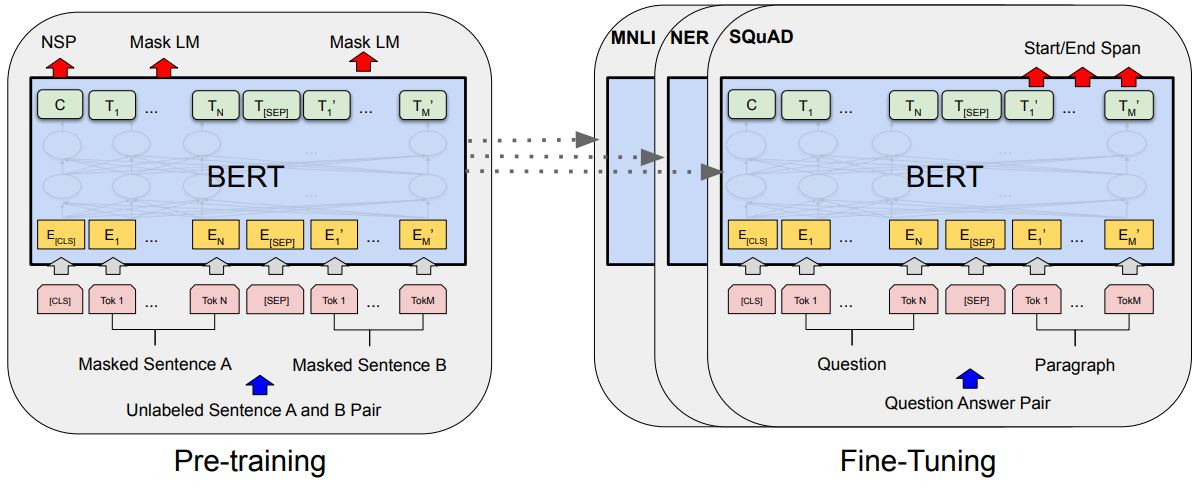
\includegraphics[scale=.5]{figures/bert_training.JPG}}
    \caption{BERT's pre-training and fine-tuning. (Source:~\cite{devlin-etal-2019-bert})}
    \label{fig:bert_training}
\end{figure}

Until now, we only talked about the strengths of BERT. However, the high quality of the text representation is achieved at the expense of high resources usage. BERT's model comes originally in two versions: BERT base (110M parameters) and BERT large (340M parameters). These model sizes require high memory capabilities and make the training procedure not accessible to everyone. For this reason, different new versions have been proposed over the last few years and several examples can be found at HuggingFace\footnote{https://huggingface.co/models}. Among these versions, we can find BERT-based models which are lighter than the original (e.g., DistilBERT, RoBERTa, etc.) and models fine-tuned for specific tasks or different languages.



\subsubsection{DistilBERT}
As suggested by the name, DistilBERT is a distilled version of BERT~\cite{distilbert}. With 40\% fewer parameters, it is 35\% faster at inference time and it is effective at 97\% with respect to the performance of the original version of BERT. Thanks to its lighter architecture composed of only 6 transformer encoders, it can be fine-tuned in a more reasonable time. DistilBERT model is pre-trained using knowledge distillation. This procedure is a compression technique in which a smaller \textit{student} model (i.e., DistilBERT) is trained to emulate a larger \textit{teacher} model (i.e., BERT).

\subsubsection{Adapters}
The fine-tuning of a model requires less time than training it from scratch. However, even this procedure can be quite expensive, especially when dealing with very large models. An alternative solution to adapt a BERT-based model to a new task can be found in the \textit{adapters}~\cite{pfeiffer-etal-2020-mad,pfeiffer2021adapterfusion}. The key concept behind the adapters is to introduce a small set of learnable parameters for each transformer layer. In the case of BERT and its variants, these parameters are added to each transformer encoder. The training is then performed by freezing all the weights of the pre-trained language model and updating only the parameters introduced by the adapters. As shown in Figure~\ref{fig:adapters}, the new parameters can be added following two strategies:
\begin{itemize}
    \item \textbf{Pfeiffer:} an adapter is added after each transformer encoder (Figure~\ref{fig:adapters_pfeiffer})
    \item \textbf{Houlsby:} two adapters are added for each transformer encoder, one after the attention layer and one after the feedforward layer (Figure~\ref{fig:adapters_houlsby})
\end{itemize}

\begin{figure}[H]
     \centering
     \begin{subfigure}[b]{0.3\textwidth}
         \centering
         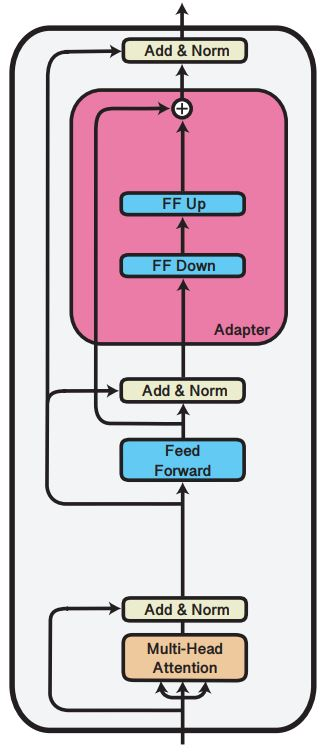
\includegraphics[width=\textwidth]{figures/adapters_pfeiffer.JPG}
         \caption{Pfeiffer strategy}
         \label{fig:adapters_pfeiffer}
     \end{subfigure}
     \hspace{40px}
     \begin{subfigure}[b]{0.302\textwidth}
         \centering
         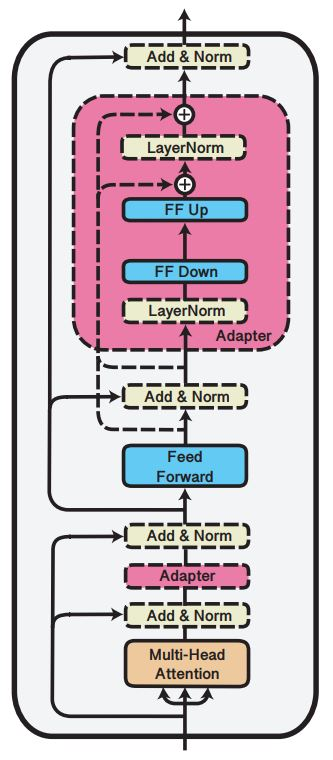
\includegraphics[width=\textwidth]{figures/adapters_houlsby.JPG}
         \caption{Houlsby strategy}
         \label{fig:adapters_houlsby}
     \end{subfigure}
    \caption{Adapters architectures. (Source:~\cite{pfeiffer2021adapterfusion})}
    \label{fig:adapters}
\end{figure}

The modifications introduced by both the architectures can be seen as the addition of auto-encoders to the model. The dimensionality of the input is reduced (with respect to a customizable reduction factor) through a first feedforward layer (FF-DOWN in Figure~\ref{fig:adapters}) and then expanded to its original size through another feedforward layer (FF-UP in Figure~\ref{fig:adapters}). In this way, a pre-trained model can adapt to new tasks without requiring any fine-tuning of the original weights. In addition, Pfeiffer et al. show in~\cite{pfeiffer2021adapterfusion} that their approach outperforms traditional strategies such as full fine-tuning as well as multitask learning.
\subsection{Entity Typing} \label{entity_typing}
\subsubsection{Overview}
Entity Typing (ET) is a subtask of Named Entity Recognition (NER) originally proposed in the 90s~\cite{MUC6}. ET aims to assign types\footnote{synonyms that could be used in this work: labels, classes} from a type set to named entities appearing in a text. Given a type set $T$, a sentence $S = c_{L} + m + c_{R} $ where $m$ is the mention span and $c_{L/R}$ is the left/right context, the goal of ET is to predict the correct types $t_{m} \subseteq T $ that better describe $m$ with respect to $S$. Since $t_{m}$ may contain multiple types, the ET task is considered a multiclass multilabel classification problem~\cite{lopez2020fully}.

Figure~\ref{fig:et_pipeline} shows the steps involved in a generic problem of ET. The input sentence requires to classify the mention of ``George Washington" with respect to the given context. Before feeding any machine learning model, the text must be transformed into a machine-readable format. This step can be based on the extraction of handcrafted features or, for most approaches from recent years can rely on newer encoding strategies ranging from Word2Vec to BERT. Finally, the preprocessed input is provided to the model that produces an output vector containing the predictions for each type in $T$. Depending on the adopted model, ET approaches can be grouped into two main categories: classification approaches like~\cite{yosef-etal-2012-hyena, Ling2012FineGrainedER, shimaoka2016attentive, choi, xu-barbosa-2018-neural}, or regression approaches like~\cite{yogatama-etal-2015-embedding, abhishek-etal-2017-fine, lopez-etal-2019-fine, ren-etal-2016-afet}.

\begin{figure}[H]
    \centering
    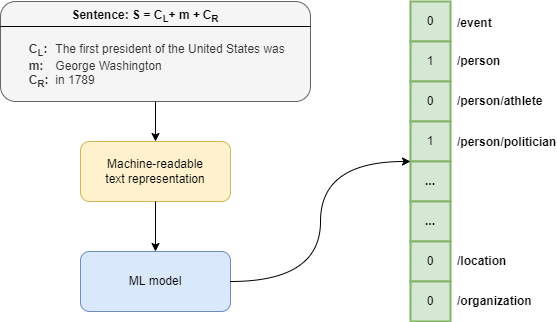
\includegraphics[width=.8\linewidth]{figures/et_pipeline.png}
    \caption{ Entity typing pipeline }
    \label{fig:et_pipeline}
\end{figure}

Using ET to detect the semantic classes of named entities can be beneficial for several NLP applications such as Question Answering, Knowledge Base Population, Relation Extraction, Entity Linking, and many others. Sometimes, the context of an NLP application requires dealing with very specific types, thus needing the extension of the typical type set composed of \verb|Person|, \verb|Organization| and \verb|Location|. For this reason, several datasets with larger type sets have been proposed over the years and used to evaluate such tasks~\cite{Ling2012FineGrainedER, ren2016noise, choi, ontonotes}. When the type set has a high cardinality, the ET task takes the name of Fine-Grained Entity Typing (FET). The type set of a FET dataset is usually organized in a hierarchical way, where the relations between coarse types and fine-grained types are represented by the edges of a tree. Each coarse type can be seen as the root node of a tree. Regarding the fine-grained types, they are represented as the descendants of the root: the deeper the node, the finer the type. The relations expressed by these hierarchical trees are the type dependencies we want to exploit in this thesis using Neural-Symbolic Integration.

\subsubsection{Approaches that exploit hierarchical information}
% specialized models
As discussed in the introduction, exploiting the hierarchy is a technique used by different approaches to face FET tasks. In~\cite{rahman2010} a model is trained to predict one branch of the hierarchy and one model per branch is trained to specialize the classification, obtaining 30 models. Similarly,~\cite{yosef-etal-2012-hyena} defines a classifier for each type and uses them following the hierarchy in a top-down manner. 

% logit filtering techniques based on hierarchy
\cite{yogatama-etal-2015-embedding,ma-etal-2016-label,ren-etal-2016-afet} defines a single classifier for all types, but filter the predictions using the hierarchy in a top-down manner, filtering out the types that are not descendants of already predicted types. The differences between these approaches reside in the inference technique:~\cite{yogatama-etal-2015-embedding} uses a fixed threshold; ~\cite{ma-etal-2016-label} a relative threshold;~\cite{ren-etal-2016-afet} infers the type with the maximum logit along with its brothers, then processes the sons of the inferred type until the bottom of the hierarchy is reached or the maximum is lower than a fixed threshold. The inference method of ~\cite{ren-etal-2016-afet} is used also by~\cite{abhishek-etal-2017-fine,ren2020FETHI}.

% hierarchy in the model/optimization
\cite{ma-etal-2016-label,ren-etal-2016-afet,shimaoka2016neural,murty-etal-2018-hierarchical,xu-barbosa-2018-neural,lopez-etal-2019-fine,wu2019,ren2020FETHI,chen-etal-2020-hierarchical} inject hierarchical information in the model through type representation and/or optimization techniques.~\cite{ma-etal-2016-label,shimaoka2016neural} represent each type through a one-hot vector with values $1$ for the type and for its ancestors.~\cite{ren-etal-2016-afet,wu2019} use hierarchy to derive similarities between types, thus weighting the errors.~\cite{murty-etal-2018-hierarchical} represent each type with a vector obtained with Rescal~\cite{Nickel2011Rescal} or ComplEx~\cite{trouillon2016complex}, thus injecting also hierarchical information about types.~\cite{xu-barbosa-2018-neural} boost the prediction of a node based on its ancestors.~\cite{lopez-etal-2019-fine,ren2020FETHI} use a layer to predict types for each level in the hierarchy, then each layer uses the higher level prediction as input.~\cite{chen-etal-2020-hierarchical} use the hierarchy to select hard negatives for a learning-to-rank training technique.

Details on how hierarchical rules are exploited in this work will be described in section~\ref{knowledge_generation}.

\subsubsection{Approaches based on BERT}
In the architecture of a FET network, the encoding of the entity mention within its context is a central characteristic of each approach. Since in our architecture BERT is central for the encoder, we now focus on the approaches that use BERT or derived language models as encoder.~\cite{wang2020} tested different contextual encoders by fixing an architecture and showed that BERT-based encoders achieved better performance in FET. Similarly,~\cite{dai-etal-2020-semantic-relations,liu-etal-2021-fine,onoe-etal-2021-modeling} use BERT as encoder to obtain a contextual vector from the input mention within its context.~\cite{dai-etal-2021-ultra} use BERT to obtain types by masking the entity mention in the input sentence and optimizing the generated tokens to obtain the tokens that represent the correct types. Finally, ~\cite{Hou2021} uses an ensemble encoder comprising SpanBERT~\cite{joshi-etal-2020-spanbert}.

Details on the FET network architecture designed for the experiments of this thesis will be presented in sections~\ref{baseline_model}.

\subsection{Fuzzy Logic} \label{fuzzy_logic}
Fuzzy Logic (FL) aims at modeling the human reasoning system. It finds its roots in multi-valued logic, which extends the classical two-valued logic by adding new truth values. Differently from other multi-valued logics which have a finite number of truth values, in FL a variable can assume the value of any real number in [0,~1], where 0 means completely false and 1 means completely true.
% This characteristic is also found in Probabilistic Logic, where the truth value of a formula is computed by probabilistic expressions.
If we think about the definition of logic, it \emph{``is the science of the formal principle of reasoning"}. From this perspective, FL is concerned with the formal principles of \textit{approximate reasoning}, since we deal with imprecise premises from which we derive imprecise conclusions~\cite{pal1991fuzzy}. This aspect reflects the fact that in human reasoning we have to deal with vagueness when classifying concepts such as a \textit{tall person} or a \textit{small number}~\cite{hajek1998basic, novak2012mathematical}. In this work, we will focus on the fuzzy extension of the First Order Logic (FOL).

Several FL implementations have been proposed over the years to approximate the logical operators and quantifiers in different ways. We now proceed with the description of some popular variants of the FL by assuming familiarity with the basic notions of the FOL. The definitions we will use in this section are taken from~\cite{analyzingDiffFuzzyLogic}. First of all, the semantics of the main fuzzy operators relies on the following functions:
\begin{itemize}
    \item \textbf{Fuzzy Negation:} function to compute the \textit{negation} of a truth value of a formula. A \textit{fuzzy negation} is a decreasing function $ N:[0,1]\rightarrow [0,1] $ \\
    such that $ N(1)=0 $ and $ \forall (x)\in [0,1], N(N(x)) \geq x $. $N$ is called \textit{strict} if it is strictly decreasing and continuous, and \textit{strong} if \\$\forall x \in [0,1], N(N(x))=x$. %In general, we will consider the classical negation $N(x) = 1 - x$.
    
    \item \textbf{Triangular Norms (t-norms):} function to compute the \textit{conjunction} of two truth values of a formula. A \textit{t-norm} is a function $ T:[0,1]^{2}\rightarrow [0,1] $ that is \textit{commutative} and \textit{associative}, where $\forall x \in [0,1], T(x,\cdot)$ is increasing (\textit{monotonicity}) and $\forall x \in [0,1], T(1,x)=x$ (\textit{neutrality}).
    
    \item \textbf{Triangular Conorms (t-conorm):} function to compute the \textit{disjunction} of two truth values of a formula. A \textit{t-conorm} (also known as s-norm) is a function $S:[0,1]^{2} \rightarrow [0,1] $ that is \textit{commutative} and \textit{associative}, where $\forall x \in [0,1], S(x,\cdot)$ is increasing (\textit{monotonicity}) and $\forall x \in [0,1], S(0,x)=x$ (\textit{neutrality}). Since t-conorms are obtained from t-norms by applying De Morgran's law from classical logic, it is possible to write the following equivalence
    \begin{gather*}
        S(a, b) = 1 - T(1 - a, 1 - b)
    \end{gather*}
    
    \item \textbf{Aggregation Operators:} function to compute $\forall$ and $\exists$ quantifiers. 
    \begin{itemize}
        \item the $\forall$ quantifier can be interpreted as a function $A:[0,1]^{n} \rightarrow [0,1] $ computed as a conjunction over all arguments $x$, using a t-norm adapted to $n$-dimensional input:
        \begin{gather*}
            A_{T}()=0 \\
            A_{T}(x_{1},x_{2},...,x_{n}) = T(x_{1},A_{T}(x_{2},...,x_{n}))
        \end{gather*}
        
        \item the $\exists$ quantifier can be interpreted as a function $E:[0,1]^{n} \rightarrow [0,1] $ computed as a disjunction over all arguments $x$, using a t-conorm adapted to $n$-dimensional input:
        \begin{gather*}
            E_{S}()=0 \\
            E_{S}(x_{1},x_{2},...,x_{n}) = S(x_{1},E_{S}(x_{2},...,x_{n}))
        \end{gather*}
    \end{itemize}
\end{itemize}

Starting from these definitions, we can find a variety of implementations of fuzzy operators. In Table~\ref{tab:fuzzy_norm} are reported the operators of some popular fuzzy logics. The variants proposed by Łukasiewicz and Gödel can be considered among the most popular, but there are many other interpretations (e.g., Weber, Yager, Fodor). Table~\ref{tab:fuzzy_aggregation} reports some aggregation operators based on the presented t-norm and t-conorm operators. 


\begin{table}
\centering
\caption{Some common t-norm and t-conorm in fuzzy logic}
\label{tab:fuzzy_norm}
\begin{tabular}{|c|cc|}
\hline
\textbf{Name} & \multicolumn{1}{c|}{\textbf{T-norm}} & \textbf{T-conorm}              \\ \hline
Gödel         & $T_{G}(a,b)=min(a,b)$                & $S_{G}(a,b)=max(a,b)$          \\ \hline
Product       & $T_{P}(a,b)=a \cdot b$               & $S_{P}(a,b)=a + b - a \cdot b$ \\ \hline
Łukasiewicz   & $T_{L}(a,b)=max(a+b-1,0)$            & $S_{L}(a,b)=min(a+b,1)$        \\ \hline
\end{tabular}
\end{table}

\begin{table}
\centering
\caption{Some common aggregation operators in fuzzy logic}
\label{tab:fuzzy_aggregation}
\resizebox{\columnwidth}{!}{\begin{tabular}{|c|cc|}
\hline
\textbf{Name}     & \multicolumn{1}{c|}{\textbf{Generalizes}} & \textbf{Aggregation operator}                                     \\ \hline
Minimum           & $T_{G}$                                   & $A_{T_{G}}(x_{1},...,x_{n}) = min(x_{1},...,x_{n})$               \\
Product           & $T_{P}$                                   & $A_{T_{P}}(x_{1},...,x_{n}) = \prod_{i=1}^{n} x_{i}$              \\
Łukasiewicz       & $T_{L}$                                   & $A_{T_{L}}(x_{1},...,x_{n}) = max(\sum_{i=1}^{n} x_{i}-(n-1), 0)$ \\ \hline
Maximum           & $S_{G}$                                   & $E_{S_{G}}(x_{1},...,x_{n}) = max(x_{1},...,x_{n})$               \\
Probabilistic Sum & $S_{P}$                                   & $E_{S_{P}}(x_{1},...,x_{n}) = 1 - \prod_{i=1}^{n} (1 - x_{i}) $   \\
Bounded Sum       & $S_{L}$                                   & $E_{S_{L}}(x_{1},...,x_{n}) = min(\sum_{i=1}^{n} x_{i}, 1)$       \\ \hline
\end{tabular}}
\end{table}
\subsection{Neuro-Symbolic Integration} \label{neuro_symbolic_integration}

\subsubsection{Symbolic vs non-symbolic}
In the last decade, the use of Deep Neural Networks (DNN) gained popularity in any machine learning context with very promising results. However, the need for better soundness and trustworthiness, as well as a better understanding of neural models, led the research community to investigate new methodologies to bring these aspects into the deep learning world. Several new methods to integrate knowledge and DNN have emerged in recent years with this ambition. This line of research is called \textit{Neuro-Symbolic Integration}~(NSI) and it represents a hot topic in the AI community~\cite{3rdWave}. The name combines the terms \textit{neural} and \textit{symbolic}, which respectively refer to neural networks and symbolic reasoning. More in detail, this research area aims to take benefits from both these two subfields of AI to support each other and overcome their limitations.

Starting from DNNs, it is well known they need a big amount of labeled training examples to generalize well. Unfortunately, such quantities of annotated data are not always available due to the big effort needed to be produced. Another limitation is that they lack interpretability because the learned functions are seen as not explainable black-boxes by humans. Furthermore, an issue that may occur when dealing with DNNs is the distributional shift (i.e., the different distribution between the training examples and the real-world data). Moving on to symbolic approaches, they do not suffer from the previous problems. Indeed, they can easily generalize through logical rules without the need for large data. Moreover, they are explainable thanks to the high-level interpretability of the logical knowledge provided by a domain expert. However, concerning DNNs, these kinds of approaches are heavily influenced by noise and are not as efficient as the neural ones.

Depending on the task for which it is designed, an NSI system can combine the symbolic and non-symbolic elements in several ways as we will see in the next section.

\subsubsection{Neuro-Symbolic Integration approaches} \label{nsi_approaches}
The first boundary between NSI approaches can be drawn with respect to the field for which they are designed. We can identify two main areas where these approaches are applied: machine learning and symbolic reasoning. In the first case, the integration aims to regulate the learning process with the use of logical knowledge. The goal of this family of approaches is to exploit the computational efficiency of DNNs and the expressiveness of logic to improve neural model capabilities in classical machine learning tasks, ranging from classification (e.g., binary, multiclass, multilabel, collective) to embedding learning, also covering relational learning tasks. On the other hand, we can find NSI approaches that are designed to solve problems from the symbolic field. In this second family of approaches, a DNN is trained to learn and perform symbolic reasoning over knowledge. The target of these works is more about Inductive Logic Programming (ILP) tasks and related.

Another possible distinction between NSI works concerns the adopted logical language. Looking at the approaches proposed in the literature, we can notice that there is not a standard way to represent logical knowledge. In most cases, a set of FOL rules is used to set constraints on data. However, a lot of approaches relying on this kind of rules apply some restrictions to the language, thus limiting its expressiveness. Such restrictions may involve the arity of predicates, functions, and logical operators. Other limitations may be imposed on the form that must be used to express logical rules (e.g., Horn clauses). Furthermore, additional assumptions can involve the usage of variable quantifiers (e.g., universal assumption). Most of these restrictions do not affect the approaches based on propositional logic. However, propositional logic is less expressive and flexible than FOL by definition.

Even the semantics of the logical language can differ a lot from one approach to another. If the goal is to have an end-to-end fully differentiable architecture, then it will be necessary to move away from finite-valued logic. The motivation behind this need derives from the nature of neural networks, which deal with continuous real values. For this reason, the most frequent solution is to relax the logic by adopting fuzzy/probabilistic semantics. In this way, it is possible to evaluate logical formulas grounded with values coming from a neural network. The main benefit that derives from the use of infinite-valued logic is that it allows to efficiently train a Neuro-Symbolic model using back-propagation algorithms. As discussed in section \ref{fuzzy_logic}, there are many possible choices between fuzzy operators. Each of them behaves in different ways when used in a differentiable learning setting. In~\cite{analyzingDiffFuzzyLogic} several experiments were performed to show the weakness and strengths of different fuzzy operators.

After this NSI overview about logical language and semantics, we can go deeper and categorize the state-of-the-art works. As proposed in~\cite{ltn}, a reasonable way to group the novel approaches is to consider the methodology adopted to inject logical knowledge into the learning process. In Figure~\ref{fig:sota} we can see three main groups. Each of them is based on different architectures.
\begin{figure}
    \centerline{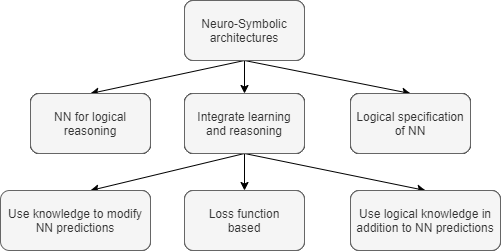
\includegraphics[scale=.58]{sota.png}}
    \caption{Categorization proposed in~\cite{ltn} to group Neuro-Symbolic approaches based on the knowledge injection methodology}
    \label{fig:sota}
\end{figure}
\\\\
\textit{\textbf{Neural architectures for logical reasoning:}}~\cite{tensorlog,cohen2020scalable,conditionalTheoremProvers,campero2018logical,neuralMarkovLogicNetworks,probabilisticLogicNeuralNetworks,recursiveReasoningNetworks,deepProlog,satnet,nlrl}. These approaches use neural networks to perform probabilistic inference on logical theories by learning reasoning strategies. This category focuses mainly on ILP (e.g., theory learning, theory compression, logical rule induction) and structured data-related tasks (e.g., knowledge graph completion, knowledge graph reasoning, triple classification). The proposed methodologies reach their goals in various ways.

Starting from~\cite{probabilisticLogicNeuralNetworks}, we find Probabilistic Logic Neural Networks. The proposed models are defined to perform knowledge graph reasoning. A Markov Logic Network~\cite{markovLogicNetworks} is used to compute the joint distribution of all triplets, then a model is trained with a variational expectation-maximization algorithm. Another approach based on Markov Logic Networks is~\cite{neuralMarkovLogicNetworks}, in which a statistical relational learning system is proposed to learn the implicit representation of FOL rules through neural networks.

Going on, we find~\cite{recursiveReasoningNetworks},~\cite{campero2018logical} and~\cite{tensorlog}. All of them introduce some FOL language restrictions, supporting only unary and binary predicates. In~\cite{recursiveReasoningNetworks}, Hohenecker and Łukasiewicz introduce Recursive Reasoning Networks. In this approach, each training example is a KB composed of different facts. Models are trained on these KBs using a shared ontology, then generate embeddings of individuals. Moving on to~\cite{campero2018logical}, Campero et al. propose a task-dependent loss function. Their methodology relies on forward chaining and soft unification to perform inference. Then there is TensorLog~\cite{tensorlog}, where a subset of FOL called \textit{ptree-SDKGs} is provided to represent knowledge in a highly scalable framework for tuning parameters of probabilistic logic. 

To conclude with the last three approaches of this family, we find the methodology proposed by Cohen et al.~\cite{cohen2020scalable}, Conditional Theorem Provers (CPT)~\cite{conditionalTheoremProvers}, and SATNet~\cite{satnet}. Cohen et al. propose \textit{sparse-matrix reified KBs} to represent subjects, objects, and relations of a KB. Through these three sparse matrices, they provide an effective and scalable way to represent symbolical knowledge in neural contexts. Moving on to CPT, Minervini et al. propose a method to boost the efficiency of a model in a particular way: during the proving mechanism, the learning process aims to dynamically select only a minimal subset of rules depending on the current goal. At last, we have SATNet by Wang et al.. In this approach, a MaxSAT solver layer is used to make DNNs able to learn logical structures without explicitly specifying any logical rules. Both CPT and SATNet adopt a logical language that is function-free.
\\\\
\textit{\textbf{Logical specification of neural network architectures:}}~\cite{liftedRelationaNeuralNetworks,logicalNeuralNetworks}. In these novel approaches, a logical language is used to specify the architecture of neural networks. This peculiarity leads to better interpretability of DNNs.

In~\cite{liftedRelationaNeuralNetworks}, Sourek et al. propose Lifted Relational Neural Networks. These neural models are composed of multiple feed-forward networks (one per example) with shared weights, where each node represents a weighted clause. The methodology proposed in Logical Neural Networks~\cite{logicalNeuralNetworks} is quite different. In this case, a neural network is modeled as a graph representing the syntax tree of logical formulas. The knowledge is expressed through a function-free FOL language with \textit{weighted nonlinear logic} semantics.

In both approaches, clause weights are learnable parameters. This feature makes the model able to give greater importance to the more relevant rules at prediction time.
\\\\
\textit{\textbf{Neuro-symbolic architectures for the integration of inductive learning and deductive reasoning:}} The goal of this group of approaches is to integrate neural and logical components into a unique (possibly fully differentiable) framework. In this way, the processes of learning and reasoning of the two components influence each other to enhance the quality of predictions. Unlike the previous categories, these works are more oriented to exploit logical knowledge in classical machine learning tasks. This family of architectures can be further divided into three subclasses:
\begin{itemize}
    \item \textbf{\textit{Logical knowledge to modify neural networks predictions:}}~\cite{liSrikumar,rnm,dlm,kenn}. These works rely on additional components (e.g., neurons, layers, modules) responsible for handling the logical knowledge.
    
    Li and Srikumar~\cite{liSrikumar} propose a framework to introduce constraints as logical statements without adding any extra learnable parameters. The base neural model is augmented with \textit{named neurons} corresponding to the predicates of the logical clauses. The post-activation value of a named neuron can be seen as the truth value of the mapped predicate. About the language, rules must be expressed as logical implications with some restrictions: the antecedent is a conjunction/disjunction of literals and the consequent is a single literal. 
    
    The second approach of this family is the one proposed by Daniele and Serafini with Knowledge Enhanced Neural Networks (KENN)~\cite{kenn}. The logical knowledge is injected through an additional layer called \textit{Knowledge Enhancer}. The initial predictions of the base neural network are modified through this layer to increase the satisfaction of each clause by applying a boost function. The logical language is a restricted function-free FOL: operators are limited to disjunction and negation, predicates must be at most binary, and variables are universally quantified.
    
    Proceeding with the last two approaches, we have Deep Logic Models (DLM)~\cite{dlm} and Relational Neural Machines (RNM)~\cite{rnm} that are quite similar in the way they work. In both cases, the process to compute the output is performed in two phases: a low-level stage to process the input and a semantic stage to perform high-level reasoning. The base neural network is supported by an undirected graphical model that represents the probability distribution. The two components are combined as follows: given the output of the neural network and the set of logical rules, a maximum a posteriori estimate (MAP) is performed to find the most probable assignment to the grounding atoms. The authors of RNM point out that their approach overcomes some limitations of DLM in terms of scalability and applicability. Furthermore, they promise a tighter connection between the trainer and the reasoner.
    
    \item \textbf{\textit{Loss function based:}}~\cite{lyrics,marra2019t,dl2,ltn,sbr,semanticLoss,harnessingDeepNeuralNetworks}. The idea behind these methodologies is to inject logical knowledge into the learning process through the loss function. The common strategy consists in translating logical rules into a regularization term to influence the training process: if the logical constraints are not satisfied during the optimization, then the regularization term will increase the loss.
    
    Starting from~\cite{semanticLoss}, Xu et al. propose a \textit{semantic loss function} to maximize the probability that the provided logical knowledge is true. In this approach, logical formulas are expressed with propositional logic. Going on we find Semantic-Based Regularization (SBR)~\cite{sbr} by Diligenti et al., where the authors propose a multilayer architecture: a kernel machine is used as the base model and a neural network is used to approximate fuzzy predicate logic
    
    Another approach we have to mention Logic Tensor Networks (LTN) by Badreddine et al.~\cite{ltn}. LTN can be used in a wide range of machine learning applications. The authors propose the language of \textit{Real Logic} to express FOL formulas. Predicates are represented as multiple neural networks and the final predictions are obtained by aggregation. LTN also includes in its features guarded quantifiers, explicit domain declarations, and different reasoning modalities. Moreover, it can be used as a generative model thanks to its ability to learn logical functions.
    
    Another interesting approach is proposed by Marra et al. with LYRICS~\cite{lyrics}. Inspired by SBR and LTN, it defines a declarative language that is suitable for exploiting logical knowledge in any machine learning context. The same authors extended this work in~\cite{marra2019t} by introducing a novel class of loss functions. These functions are specified through a \textit{t-norm generator} that leads to faster convergence. The difference can be found in the way the satisfaction of the knowledge is computed: instead of computing the truth degree of each subformula, connectives and quantifiers are used to combine the loss values in a less costly way.
    
    Hu et al. propose in~\cite{harnessingDeepNeuralNetworks} a different methodology to influence the optimization procedure. A distillation strategy is used to train the model: while the teacher network is trained in a semi-supervised setup to learn from unlabeled examples, the student network is trained to emulate the teacher and, at the same time, to predict some labeled examples.
    
    The latest approach of this category is proposed by Fischer et al. with DL2~\cite{dl2}. The model optimization is performed through an optimizer-adversary game: while the optimizer is trained to meet the constraints, the adversary is trained to find counterexamples that contradict the knowledge. Regarding the language, the knowledge is expressed through numerical comparisons linked by logical operators. This particular way of defining the knowledge makes this approach suitable to capture constraints in regression tasks.
    
    \item \textbf{\textit{Logical knowledge applied to neural networks predictions:}}~\cite{abl,deepproblog,li2020closed}. These approaches are used to compute logical inference starting from the output of a base neural network. The final output corresponds to the consequences implied by the neural predictions.
    
    In ABL~\cite{abl} by Dai et al., the output of a base neural network is extended using abductive reasoning. The goal is to maximize the consistency between predictions and background knowledge. Given the background knowledge, the consistency optimization process is performed to revise the pseudo-labels produced by the network taking into account the hypotheses obtained through logical abduction.
    
    Li et al.~\cite{li2020closed} provide an alternative architecture to process and update neural network predictions. A grammar model is introduced to bridge the neural model and the symbolic reasoning module. Errors are propagated through a back-search algorithm to find the most probable corrections that will be used as pseudo-labels.
    
    The last approach we find is DeepProbLog~\cite{deepproblog}, proposed by Manhaeve et al. as an extension of ProbLog. The goal of this work is to adapt ProbLog to deal with the output of a neural network. In this way, the predicates assume a neural interpretation. The logical knowledge is expressed through a function-free language in the form of a Prolog program, i.e., a set of Horn clauses.
\end{itemize}

\paragraph{Approaches of interest}
After this broad overview of possible NSI approaches, we can focus on those best suited to Fine-grained Entity Typing. In section~\ref{entity_typing}, FET has been described as a multilabel multiclass problem where hierarchical dependencies occur between types. Given this premise, the approaches that explicitly support multilabel classification are LTN~\cite{ltn}, SBR~\cite{sbr}, LYRICS~\cite{lyrics}, KENN~\cite{kenn} and RNM~\cite{rnm}. During the categorization, we saw that LTN, LYRICS, and SBR, belong to the group of methods based on the loss function. On the contrary, KENN and RNM both have a post-elaboration step to modify the final predictions. A detailed comparison between loss-based approaches, KENN and RNM can be found in~\cite{daniele2021neural}. The more relevant differences will be highlighted below.

KENN is the most recent of the five approaches identified. As stated by its authors, the strategy used by KENN affects the Hypothesis Space (HS) differently from loss-based approaches: while the action of constraining the loss function can be seen as ``removing" solutions from the HS, the action of KENN will result in the opposite. In other words, LTN, LYRICS, and SBR will produce models where the solutions penalized at training time can no longer be obtained at inference time. On the other hand, the additional layer introduced by KENN keeps influencing the model at inference time by adding new solutions to the HS. Moving on to RNM, we can find a relevant difference with respect to KENN in the optimization of the clause. The methodology applied by RNM considers the entire logical knowledge, while KENN optimizes each clause separately. As we will see when presenting KENN in section~\ref{KENN}, the independent optimization of the logical clauses may produce the side effect of not fully exploiting the knowledge during the training process.

All these works adopt a language that allows expressing FOL formulas. KENN is the only one having restrictions on the usage of connectives, quantifiers, predicates, and functions. However, these limitations still allow expressing the hierarchical relations of interest for FET. About the evaluation of a logical clause, each approach computes the truth degree of a formula using fuzzy operators. This feature makes it possible to build an end-to-end fully differentiable architecture except for RNM, which needs to solve an optimization problem at inference time.

An important feature to consider about an NSI system is the ability to learn clause weights. While KENN and RNM let you set clause weights as learnable parameters, LYRICS and SBR only support fixed weights. In LTN it is not possible to specify weights, but the authors suggest adding them indirectly to a clause by the conjunction of a 0-ary predicate. The feature of learning clause weights may be really helpful when dealing with multilabel classification problems because label dependencies are often unknown. In these cases, we can use a set of automatically generated rules and delegate to the network the choice of optimal weights. The learning process will decrease the weights of the clauses that are inconsistent with the data until they become irrelevant and, at the same time, it will increase the weights of the consistent ones.

The summary of the differences between the analyzed approaches can be found in Table~\ref{tab:sota_comparison}.

\begin{table}[H]
\centering
% \small
\caption{Comparison of KENN, RNM, LYRICS, LTN and SBR main characteristics}
\label{tab:sota_comparison}
\resizebox{\columnwidth}{!}{\begin{tabular}{c|c|c|c|c|c|}
\cline{2-6}
                                                          & \textbf{KENN}                                                                                                        & \textbf{RNM} & \textbf{LYRICS} & \textbf{LTN} & \textbf{SBR} \\ \hline
\multicolumn{1}{|c|}{\textbf{Knowledge}}                  & FOL                                                                                                                  & FOL          & FOL             & FOL          & FOL          \\ \hline
\multicolumn{1}{|c|}{\textbf{Semantics}}                   & fuzzy                                                                                                                & fuzzy        & fuzzy           & fuzzy        & fuzzy        \\ \hline
\multicolumn{1}{|c|}{\textbf{Restrictions / Assumptions}} & \begin{tabular}[c]{@{}c@{}}- only disjunction\\ and negation\\ - no parenthesis\\ - universal assumption\end{tabular} & none         & none            & none         & none         \\ \hline
\multicolumn{1}{|c|}{\textbf{Predicates}}                 & unary and binary                                                                                                     & n-ary        & n-ary           & n-ary        & n-ary        \\ \hline
\multicolumn{1}{|c|}{\textbf{Functions}}                  & no                                                                                                                   & yes          & yes             & yes          & yes          \\ \hline
\multicolumn{1}{|c|}{\textbf{Clause weights}}             & learnable                                                                                                            & learnable    & fixed           & none           & fixed        \\ \hline
\end{tabular}}
\end{table}


About the effectiveness of these works, in~\cite{rnm} we can find an experimental evaluation of collective classification to compare RNM and SBR. The results show that RNM achieved better performance than SBR on Citeseer~\cite{citeseer} dataset. The same experiment is reported in~\cite{daniele2021neural} using KENN. In this case, the results show that KENN is less performing than RNM when dealing with small training sets. However, it becomes more effective when the percentage of training data increases. Another evaluation of KENN involves the datasets Yeast~\cite{yeast}, Emotions~\cite{emotions} and VRD~\cite{vrd}. On these multilabel classification datasets, KENN reached better results than LTN and other state-of-the-art solutions in almost every setup~\cite{kenn}.

Another important factor to take into account is scalability. In terms of computation, the way KENN injects the knowledge is quite simple and inexpensive with respect to the approaches that are based on the loss function. If we consider LTN as an example, expensive operations are performed at training time to compute the truth degree of a grounded formula. RNM has scalability issues too, but in this case the bottleneck can be found in the optimization problem to solve at inference time.
\\\\
To sum up, KENN has more restrictions and limitations in the language. Anyhow, its expressivity suffices to represent the logical rules of interest. The advantages coming from learnable clause weights, scalability, and effectiveness, had a heavier impact on the choice of this NSI framework. Moreover, KENN is simple to integrate and analyze, thus allowing to easily study the effect of the logical knowledge injected by each clause.


\section{Knowledge Enhanced Neural Networks} \label{KENN}

\subsection{KENN} \label{kenn_architecture}
As anticipated in section~\ref{nsi_approaches}, KENN is the Neuro-Symbolic Integration approach chosen for this study. It adopts a restricted FOL language with fuzzy semantics and injects the logical knowledge directly into the model structure by adding a special layer. This new layer acts to increase the satisfaction of the logical knowledge by modifying the final predictions of the neural network.

In this section we go deeper into the details of the framework of KENN by focusing on the most important aspects to better understand its role in this thesis.

\subsubsection{Language and semantics}
We can start by introducing more details about the logical language supported by KENN. This framework allows imposing constraints on predictions by providing a set of logical clauses that constitute our knowledge base. For the sake of brevity, we will refer to a logical knowledge base as KB. Each clause of the KB represents a logical formula generated from a subset of the FOL with the following restrictions:
\begin{itemize}
    \item \textit{the only operators allowed are disjunction and negation}
    \item \textit{parentheses are not allowed}
    \item \textit{variables are assumed to be universally quantified}
    \item \textit{only unary and binary predicates are allowed}
    \item \textit{functions are not allowed}
\end{itemize}
Even if we can use only the operators of negation and disjunction, it is possible to use logical equivalence to introduce some other operators into KENN's language. Considering classical logic for simplicity, two examples of logically equivalent formulas are:
\begin{itemize}
    \item  $ A \to B = \neg A \vee B $
    \item  $ \neg ( A \wedge B) = \neg A \vee \neg B $ (De Morgan's law)
\end{itemize}
The mapping between FOL and KENN's restricted language is quite trivial. If we consider the example of logical implication, we can schematize the translation as follows:
\begin{enumerate}
    \item Starting from the FOL formula:
    \begin{gather*}
        \forall X, A(X) \to B(X)
    \end{gather*}
    \item Remove quantifier (universal assumption):
    \begin{gather*}
        A(X) \to B(X)
    \end{gather*}
    \item Remove variables\footnote{we can remove variables because we are dealing only with unary predicates referred to the same variable}:
    \begin{gather*}
        A \to B
    \end{gather*}
    \item Use logical equivalence (when possible) to convert unsupported operators:
    \begin{gather*}
        \neg A \vee B
    \end{gather*}
\end{enumerate}
Now that we transformed the FOL formula into a clause supported by KENN, we have to convert it using the syntax required by the parser:
\begin{enumerate}
    \item Use ``n" as negation symbol and ``," to represent disjunctions:
    \begin{gather*}
        nA,B
    \end{gather*}
    \item Add a positive clause weight; use ``\_" in case you want to set it as learnable parameter:
    \begin{gather*}
        0.5:nA,B
    \end{gather*}
\end{enumerate}

The semantics of KENN's logic is fuzzy. The authors propose the \textit{Gödel’s t-conorm} as fuzzy operator to compute the truth degree of a formula. Given a clause $ c $ representing a disjunction of $ n $ literals, the value of the t-conorm is computed by:
\begin{equation*} \label{eq:godel}
    \bot(c) = \max\limits_{i=1}^{n}(c_{i})
\end{equation*}
According to the equation, we can remark that the satisfaction of a clause depends exclusively on the value of the highest literal appearing in it.


\subsubsection{Architecture}
Moving on to KENN's architecture, we already saw in section \ref{nsi_approaches} that it differs from most of its competitors that inject knowledge through the loss function. The idea behind this approach is to have an additional layer that is responsible for injecting knowledge. This layer is simply put on top of an arbitrary neural network and becomes an integral part of it, thus influencing both the learning process and the predictions at inference time according to the provided logical knowledge. The architecture of KENN is represented in Figure~\ref{fig:kenn_architecture} at the maximum abstraction level.

\begin{figure}[H]
    \centering
    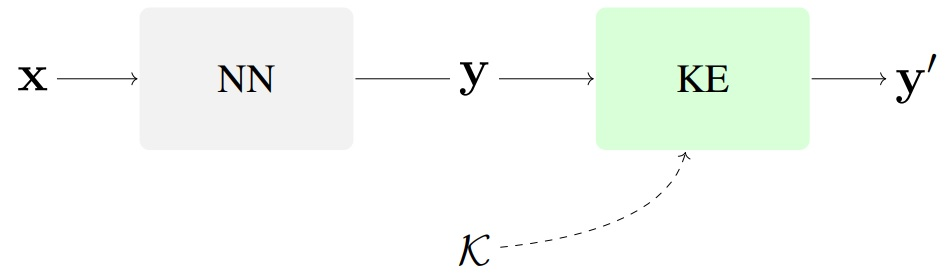
\includegraphics[width=.7\linewidth]{kenn_architecture.jpg}
    \caption{ Architecture of KENN - Features $ x $ are given in input to a neural network (NN), the predictions $ y $ are modified by the Knowledge Enhancer (KE) to satisfy a logical KB ($ \kappa $), thus obtaining the final predictions $ y'$. (Source:~\cite{kenn})}
    \label{fig:kenn_architecture}
\end{figure}

\paragraphn{Components}
As we can see from the Figure~\ref{fig:kenn_architecture}, the main component of the architecture is the Knowledge Enhancer, which has a specific role and is composed of a set of subcomponents that cooperate:
\begin{itemize}
    \item \textbf{Knowledge Enhancer (KE):} The KE is the layer responsible for injecting logical knowledge into the model. Given a logical KB $K$ composed of $n$ clauses, the KE contains $n$ independent \textit{Clause Enhancers} that produce $n$ variations to modify $y$ accordingly to $K$. These variations, also called deltas, are aggregated by the KE to obtain the enhanced output $y'$.
    \item \textbf{Clause Enhancer (CE):} The CE is the unit responsible for increasing the satisfaction of a clause by applying a \textit{boost function}, which acts on the predictions of the labels related to the literals of the clause. Each CE is associated to a clause weight $w_c$ that regulates the influence of the clause during the enhancement process.
    \item \textbf{T-conorm boost function (TBF):} The TBF is the function applied by each CE to increase the value of the Gödel t-conorm of its grounded clause. The TBF produces the deltas that will be aggregated by the KE to obtain the final predictions. Since the TBF is based on the Gödel t-conorm, which is non-differentiable, the authors propose the following soft differentiable approximation to compute the deltas:
    \begin{equation} \label{eq:tbf}
    	\delta _{w_{c}}(v)_{i} = w_{c} \cdot softmax(v)_{i}
    \end{equation}
    where $ w_{c} $ is the weight of the clause $ c $, $ v $ is the preactivation vector (i.e., the output of the base neural network) of the literals belonging to $c$, and $ i $ refers to the \textit{i-th} literal of the clause.
\end{itemize}

\paragraphn{Clause Enhancer details}
Now that the high-level architecture has been presented, we can go deeper into the details of the clause enhancement mechanism. Referring to Figure~\ref{fig:clause_enhancer}, the functioning of a CE can be summarized with the following steps:
\begin{enumerate}
    \item Receive the preactivations $ z $ of all the grounded literals (i.e., the output $y$ of the base neural network).
    \item Apply a pre-elaboration step $ \phi $ to filter the preactivations: keep only the preactivations of the literals belonging to the clause $ c $ and change the sign of the preactivations of negated literals.
    \item Apply the TBF (Equation \ref{eq:tbf}) to the resulting preactivations to produce the deltas.
    \item Apply a post-elaboration step $ \phi' $ to convert the TBF’s results into changes to be applied to the original preactivations $ z $: expand back the dimensionality by filling with 0s the positions of the previously filtered out preactivations, then change back the sign of the deltas of negated literals.
\end{enumerate}
An example of clause enhancement that may help to better comprehend the mechanism is shown in Figure~\ref{fig:example_enhancement}. 
\begin{figure}[H]
    \centering
    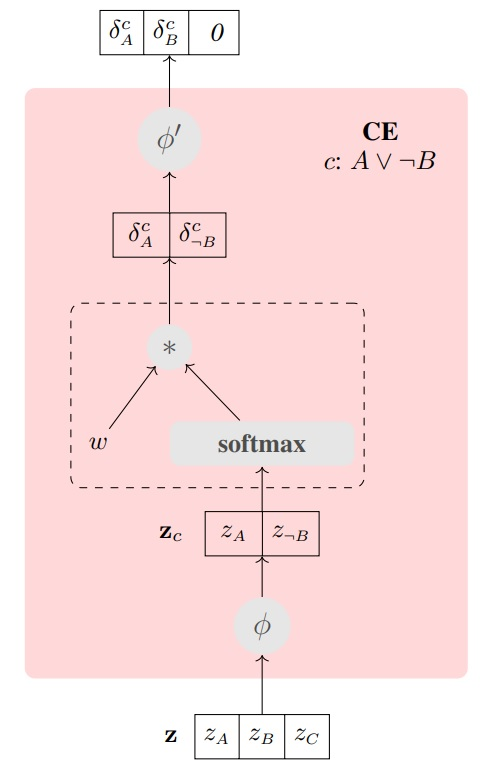
\includegraphics[width=.35\linewidth]{clause_enhancer.jpg}
    \caption{Clause Enhancer for $ A \vee \neg B $. (Source:~\cite{kenn})}
    \label{fig:clause_enhancer}
\end{figure}

\begin{figure}[H]
    \centering
    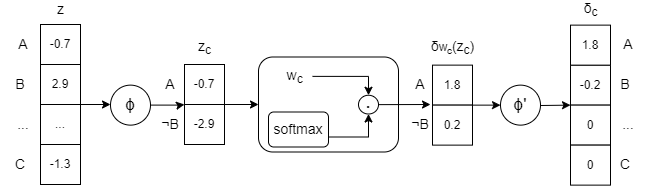
\includegraphics[width=.75\linewidth]{example_enhancement.png}
    \caption{Example of clause enhancement for $ A \vee \neg B $, with $w_{c}=2.0$}
    \label{fig:example_enhancement}
\end{figure}

\begin{figure}
    \centering
    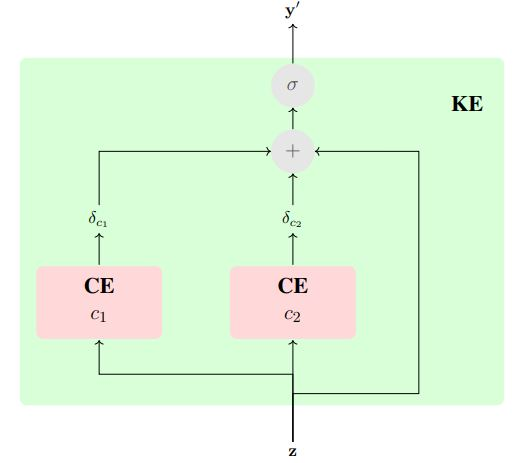
\includegraphics[width=.5\linewidth]{knowledge_enhancer.jpg}
    \caption{Knowledge Enhancer producing enhanced predictions. The deltas of each CE are summed to the preactivations of the base neural network. (Source:~\cite{kenn})}
    \label{fig:knowledge_enhancer}
\end{figure}

\paragraphn{Aggregation step}
Once understood the enhancement mechanism for a single clause, it is necessary to explain how the outputs of each CE are combined. An illustration of this step is available in Figure~\ref{fig:knowledge_enhancer}. As we can see, the KE aggregates the initial preactivations to the deltas coming from each CE. The aggregation consists of a simple sum and the resulting value is passed through an activation function to obtain the final predictions $y'$. The authors of KENN motivate the choice of the sum as it leads to faster learning and inference, thus resulting in higher scalability. However, this kind of aggregation may lead to the so-called \textit{conflicts}.

A conflict occurs when the same literal appears with different signs in two or more clauses, thus leading the CEs to produce for the same literal both positive and negative deltas. The natural consequence is that there could be side effects when performing the aggregation step since the benefits of a clause could be mitigated or completely overwhelmed by the effects of another clause. To better understand this particular situation, imagine having two clauses $ c_{1}: \neg A \vee B $ and $ c_{2}: \neg B \vee C \vee D $, where $B$ is the literal involved in possible conflicts. Let us assume that starting from an arbitrary preactivation vector $ z $ the CEs generate $ \delta (z_{c_{1}})_{B} = 0.7 $ and $ \delta (z_{c_{2}})_{B} = -0.5 $. At this point, we can aggregate the deltas obtaining $\delta _{B} = 0.7 - 0.5 = 0.2$. The result is that the final change on $ B $ will reflect the effect of the stronger grounded clause lowered by the effect of the weaker one. It is important to underline that the more literals involved in a clause, the less the probability to encounter relevant conflicts, since the same literal must be dominant in both clauses~\cite{kenn}.

\paragraphn{Enhancement of a logical implication}
An important aspect to remark and keep in mind is that since the goal of KENN is to increase the Gödel t-conorm of a grounded clause, the action of a CE is always the following: \textit{produce a positive boost to the preactivations of positive literals and a negative boost to the preactivations of negative literals}. In other words, the sign of a delta computed by the CE reflects the sign of the related literal of the clause. Thus, reminding that a logical implication must be expressed in KENN by using the logical equivalence $ A \to B = \neg A \vee B $, the effect of a CE always results in a decrease of the preactivation of $A$ and an increase of the preactivation of $B$. This means that a violated grounded clause (i.e., $ 1 \to 0 $) is always pushed by KENN towards its satisfiability (i.e., $ 1 \to 1 $, $ 0 \to 0 $, or $ 0 \to 1 $).

If we consider again the example in Figure~\ref{fig:example_enhancement}, which is based on the clause $A \vee \neg B $ that can be seen as $ B \to A $, we can analyze how the knowledge enhancement of an implication would modify the initial predictions. Table~\ref{tab:example_tbf_values} reports the values obtained at each step of the CE, plus the prediction on $A$ and $B$ before and after the enhancement. If we consider $ threshold = 0.5 $ to assign 1 and 0 to the grounded literals and we compare the columns $ \sigma (z) $ and $ \sigma (\delta _{w_{c}}(z)+ z)$, we can observe that KENN changed $1 \to 0$ into $1 \to 1$.

\begin{table}[h]
\centering
\caption{Numeric example of the action of KENN for $ A \vee \neg B $}
\label{tab:example_tbf_values}
\begin{tabular}{c|c|c|c|c|c|c|c|}
\cline{2-8}
                                 & $ z $ & $ \sigma (z) $       & $ z_{c} $ & $ \delta _{w_{c}}(z_{c}) $ & $ \delta _{w_{c}}(z) $ & $ \delta _{w_{c}}(z) + z $ & $ \sigma (\delta _{w_{c}}(z)+ z)$ \\ \hline
\multicolumn{1}{|c|}{$ A $}      & -0.7  & 0.33 ($ \approx 0 $) & -0.7      & 1.8                        & 1.8                    & 1.1                        & 0.75 ($ \approx 1 $)              \\ \hline
\multicolumn{1}{|c|}{$ B $}      & 2.9   & 0.95 ($ \approx 1 $) & -         & -                          & -0.2                   & 2.7                        & 0.94 ($ \approx 1 $)              \\ \hline
\multicolumn{1}{|c|}{$ \neg B $} & -     & -                    & -2.9      & 0.2                        & -                      & -                          & -                                 \\ \hline
\end{tabular}
\end{table}


\paragraphn{Considerations on the clause weight}
In the example above, KENN with its intervention changed the final predictions leading to a satisfied clause. This is not always the case, since the choice of a different clause weight could lead to another outcome. In Figure~\ref{fig:sigmoid_example} we can see two examples that start from the same preactivations, but use different clause weights. The examples show in a graphical way the changes introduced by KENN to the initial prediction from the perspective of the sigmoid activation function. Considering that a classification threshold of 0.5 on post-sigmoid values is equivalent to using a 0 threshold directly on preactivations, we can see that the delta produced in Figure~\ref{fig:sigmoid_example_w2} is not enough to push the prediction over the threshold. On the contrary, Figure~\ref{fig:sigmoid_example_w1} shows that the prediction changes its sign thanks to a higher clause weight.

\begin{figure}[h]
     \centering
     \begin{subfigure}{0.47\textwidth}
         \centering
         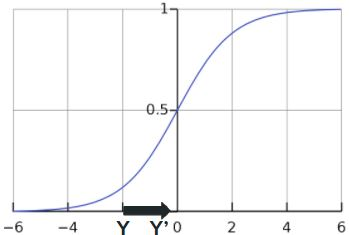
\includegraphics[width=\textwidth]{figures/ex_enhancement_w2.JPG}
          \caption{$w=2$,  $\delta_{Y} = 1.6$,  $Y'=-0.4$}
         \label{fig:sigmoid_example_w2}
     \end{subfigure}
     \hfill
     \begin{subfigure}{0.47\textwidth}
         \centering
         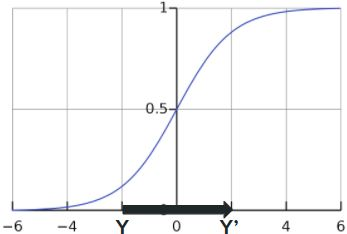
\includegraphics[width=\textwidth]{figures/ex_enhancement_w5.JPG}
         \caption{$w=5$,  $\delta_{Y} = 4$,  $Y'=2$}
         \label{fig:sigmoid_example_w1}
     \end{subfigure}
        \caption{Example of enhancement given $Y = -2$ and $softmax_{Y} = 0.8$, from the perspective of the sigmoid activation function}
        \label{fig:sigmoid_example}
\end{figure}

% \begin{table}
% \centering
% \caption{Truth table of the clause $ A \vee \neg B $}
% \label{tab:example_tbf_tt}
% \begin{tabular}{c|c|c|c|}
% \cline{2-4}
%                         & $ A $ & $ B $ & $ A \vee \neg B $ \\ \hline
% \multicolumn{1}{|c|}{1} & 0     & 0     & 1                 \\ \hline
% \multicolumn{1}{|c|}{2} & 0     & 1     & 0                 \\ \hline
% \multicolumn{1}{|c|}{3} & 1     & 0     & 1                 \\ \hline
% \multicolumn{1}{|c|}{4} & 1     & 1     & 1                 \\ \hline
% \end{tabular}
% \end{table}
\paragraphn{Relational KENN}
The authors of KENN propose also an extended version of the framework to use logical knowledge in relational domains. In that version, it is possible to specify relations between examples in contexts like collective classification by using binary predicates. The architecture of the relational version is slightly different and requires more sophisticated steps to inject logical knowledge into the neural network. The details can be found in~\cite{daniele2021neural} and will not be discussed here since this thesis focuses on the use of unary predicates.
\subsection{Preliminary experiments: encoding hierarchical rules}
Before diving into the FET task, KENN has been tested in a hierarchical classification scenario. Since the goal of this preliminary phase is to familiarize with KENN rather than achieve the best performance, we do not dwell on the architecture, training setup, and results. We focus, instead, on how hierarchical relations can be encoded with KENN. Different heuristics to represent a hierarchy through logical rules are proposed within these preliminary studies.

\subsubsection{Dataset}
% The baseline model implemented for these experiments has a simple architecture. It uses DistilBERT as encoder, followed by a dense fully connected layer and a final classification layer that applies the sigmoid activation function. The choice of this activation function is due to the fact that in a multilabel task we want as output the probability of each label. Starting from this architecture, KENN is placed between the fully connected layer and the classification layer. Clause weights are set as learnable parameters with an initial value of 0.5.

The dataset used for this experiment is called DBpedia Classes\footnote{https://www.kaggle.com/danofer/dbpedia-classes}. It is composed of approximately 240k labeled Wikipedia articles, where the only feature is the span of text. The types are organized as a forest of 9 trees, each of them representing a 3-level hierarchy. The type set counts 298 types: 9 at top-level, 70 at middle-level, and 219 at low-level. Each example is labeled with exactly 3 classes from the full path of a tree (i.e., one class per level). For example, if we consider the \textit{Species} tree shown in Figure~\ref{fig:dbpedia_classes}, an instance of the dataset could present $ label_{1} = Species $, $ label{_2} = Animal $, and $ label_{3} = Bird $.

\begin{figure}[H]
    \centering
    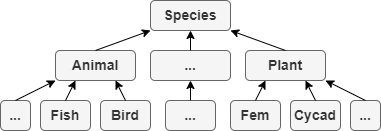
\includegraphics[width=.7\linewidth]{dbpedia_classes.png}
    \caption{Example of a tree of DBpedia Classes}
    \label{fig:dbpedia_classes}
\end{figure}

\subsubsection{Knowledge definition} \label{knowledge_generation}
The first step to integrate KENN is to create the logical KB. We can start from the tree in Figure~\ref{fig:dbpedia_classes} and then generalize different strategies for defining logical rules. The most intuitive and straightforward way consists in following the \textit{is-a} relations, which are implicitly encoded in the tree structure. Considering the picture, it is possible to state that if an instance is a \texttt{Fish}, then it is an \texttt{Animal}. In the same way, we can then proceed with the next level of the hierarchy and state that if an instance is an \texttt{Animal}, then it is a \texttt{Species}. This mechanism can be extended to all the other subtrees to create a logical clause per edge. The resulting KB will be a set of logical implications between subtypes and supertypes. Even if it seems a natural way to describe the hierarchy, it doesn't necessarily mean it is the most effective solution. For this reason, we should take a step back and analyze the alternatives offered by the hierarchy. Figure~\ref{fig:hierarchy_example} shows a generic hierarchy and highlights two groups of constraints we can distinguish:
\begin{enumerate}
    \item \textbf{Vertical constraints:} based on the paths of a tree, they can be used to represent specialization relations
    \item \textbf{Horizontal constraints:} based on pairs of nodes from different branches, they can be used to represent disjointness relations
\end{enumerate}
\begin{figure}[H]
    \centering
    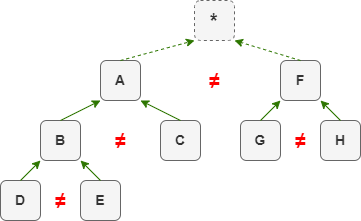
\includegraphics[width=.7\linewidth]{hierarchy_example.png}
    \caption{Examples of a generic hierarchy. In green the vertical constraints, in red the horizontal constraints.}
    \label{fig:hierarchy_example}
\end{figure}
For each group of constraints, it is possible to implement different strategies to define the KB. In the rest of the thesis, these strategies will be referred to as \textit{KB modes}. Note that in the definitions below we will use unary predicates to represent the belonging of an instance $X$ to a type.

\paragraphn{Vertical Constraints}
Using the unary predicates $Subtype$ and $Supertype$ such that the type $Subtype$ is a specialization of the type $Supertype$, we can define three main strategies to build vertical constraints:
\begin{itemize}
    \item \textbf{Bottom Up:}
        \begin{itemize}
            \item FOL: $ \forall X, Subtype(X) \to Supertype(X) $
            \item KENN: $ \neg Subtype \vee Supertype $
            \item Defined by following every path of the tree from the leaves to the root. It represents the logic dependency between types, following the most widely used semantics in the definition of subclass.
            \item Open World Assumption: a clause is satisfied even when an instance is assigned only to supertypes
        \end{itemize}
    \item \textbf{Top Down:}
        \begin{itemize}
            \item FOL: $ \forall X, Supertype(X) \to (Subtype_{1}(X) \vee ... \vee Subtype_{n}(X)) $
            \item KENN: $ \neg Supertype \vee Subtype_{1} \vee ... \vee Subtype_{n}  $
            \item Defined by following every path of the tree from the root to the leaves
            \item Closed World Assumption: a clause is not satisfied when an instance is assigned to a supertype without any of its subtypes
        \end{itemize}  
    \item \textbf{Hybrid:} 
    \begin{itemize}
        \item Composed of a mix of \textit{Bottom Up} and \textit{Top Down} clauses
    \end{itemize}
\end{itemize}
Note that if a model that uses this kind of knowledge is confident about a given type, a \textit{Bottom Up} clause propagates this certainty towards the root of the hierarchy. Conversely, a \textit{Top Down} clause only guarantees that one of the subtypes is appropriate, but provides no information as to which one. The reason, of course, is the tree-like hierarchy, where each type has only one parent, but potentially many descendants.

The presented KB modes can be considered as the starting point to create new strategies by adding some variations. In Table~\ref{tab:kb_modes} we can find a summary that comprehends every KB mode, each of them accompanied by examples of clauses from the hierarchy in Figure~\ref{fig:dbpedia_classes}. Before proceeding with the explanation of the variants, we have to make clear why they have been introduced: the conflicts. If we look at the table, we can see that in the examples of the pure \textit{Bottom Up} and \textit{Top Down} modes there are conflicts: a middle-level label appears both as positive and negative literal. This fact derives from the translation of the logical implication into a disjunction since an intermediate node is at the same time antecedent and consequent of different logical implications. This behavior still hold for the \textit{Hybrid} mode.

Now that the possible problems of the starting strategies are known, it is possible to introduce their conflict-free variants. These variants avoid conflict situations in different ways. The ``Skip" ones rely on the transitivity of a relation by linking top-level and low-level nodes by skipping those middle-level nodes that would create a conflict (i.e., a middle-level node cannot be the antecedent of an implication rule). These solutions provide a more shallow representation of the knowledge, especially for the \textit{Top Down Skip}. In this case, a logical rule that represents the relation between top-level and low-level lose effectiveness because the implication may have too many consequents. The \textit{Hybrid In} and \textit{Hybrid Out} modes, instead, avoid conflicts by fixing the middle-level types as consequent or antecedent of an implication rule, respectively. In this way, the deltas produced by each CE for the same literal will always have the same sign.

Note that the proposed variants are valid for this dataset, but some of them do not apply to every context since they require a hierarchy with at least 3 levels.

\begin{table}
\centering
\caption{Strategies for defining logical clauses based on the hierarchy in Figure~\ref{fig:dbpedia_classes}}
\label{tab:kb_modes}
\begin{tabular}{c|l|}
\cline{2-2}
                                              & \multicolumn{1}{c|}{\textbf{Clauses}}                                                                                                                                                                                             \\ \hline
\multicolumn{1}{|c|}{\textbf{Bottom Up}}      & \begin{tabular}[c]{@{}l@{}}$ c_{1}: \neg Fish \vee Animal $\\ $ c_{2}: \neg Bird \vee Animal $\\ $ c_{3}: \neg Animal \vee Species $\\ ...\end{tabular}                                                                           \\ \hline
\multicolumn{1}{|c|}{\textbf{Top Down}}       & \begin{tabular}[c]{@{}l@{}}$ c_{1}: \neg Species \vee Animal \vee ... \vee Plant $\\ $ c_{2}: \neg Animal \vee Fish \vee ... \vee Bird $\\ $ c_{3}: \neg Plant \vee Fem \vee ... \vee Cycad $\\ ...\end{tabular}                  \\ \hline
\multicolumn{1}{|c|}{\textbf{Hybrid}}         & \begin{tabular}[c]{@{}l@{}}$ c_{1}: \neg Species \vee Animal \vee ... \vee Plant $\\ $ c_{2}: \neg Animal \vee Species $\\ $ c_{3}: \neg Plant \vee Species $\\ ...\end{tabular}                                                  \\ \hline
\multicolumn{1}{|c|}{\textbf{Bottom Up Skip}} & \begin{tabular}[c]{@{}l@{}}$ c_{1}: \neg Fish \vee Animal $\\ $ c_{2}: \neg Fish \vee Species $\\ $ c_{3}: \neg Bird \vee Animal $\\ $ c_{4}: \neg Bird \vee Species $\\ ...\end{tabular}                                         \\ \hline
\multicolumn{1}{|c|}{\textbf{Top Down Skip}}  & \begin{tabular}[c]{@{}l@{}}$ c_{1}: \neg Species \vee Animal \vee ... \vee Plant $\\ $ c_{2}: \neg Species \vee Fish \vee ... \vee Bird \vee Fem \vee Cycad $\\ ...\end{tabular}                                                  \\ \hline
\multicolumn{1}{|c|}{\textbf{Hybrid In}}      & \begin{tabular}[c]{@{}l@{}}$ c_{1}: \neg Species \vee Animal \vee ... \vee Plant $\\ $ c_{2}: \neg Fish \vee Animal $\\ $ c_{3}: \neg Bird \vee Animal $\\ $ c_{4}: \neg Fem \vee Plant $\\ ...\end{tabular}                      \\ \hline
\multicolumn{1}{|c|}{\textbf{Hybrid Out}}     & \begin{tabular}[c]{@{}l@{}}$ c_{1}: \neg Animal \vee Species $\\ $ c_{2}: \neg Animal \vee Fish \vee ... \vee Bird $\\ $ c_{3}: \neg Plant \vee Species $\\ $ c_{4}: \neg Plant \vee Fem \vee ... \vee Cycad $\\ ...\end{tabular} \\ \hline
\end{tabular}
\end{table}

\paragraphn{Horizontal Constraints}
These constraints aim to avoid the co-occurrence of types whose instances form disjoint sets (e.g., if an example is labeled as \texttt{Person} it cannot be labeled as \texttt{Location} and vice versa). Using $T_i$ to indicate an arbitrary type, the logical rule that best represents this constraint is:
\begin{gather*}
    \forall X, T_{1}(X) \to (\neg T_{2}(X) \wedge ... \wedge \neg T_{n}(X))
\end{gather*}
With the following steps, we can derive an equivalent formula without implication and conjunctions:
\begin{align*}
    & T_{1} \to (\neg T_{2} \wedge ... \wedge \neg T_{n}) = \\
    & = \neg T_{1} \vee (\neg T_{2} \wedge ... \wedge \neg T_{n}) = \\
    & = \neg T_{1} \vee \neg (T_{2} \vee ... \vee T_{n})
\end{align*}
Unfortunately, the derived formula cannot be furthermore decomposed due to the presence of parentheses. We can opt for two alternative solutions to bypass the problem:
\begin{enumerate}
    \item \textbf{Approximate the rule with a softer constraint:} if an instance does not belong to \texttt{T$_1$}, then it should belong to another type. \\
    The logical formula for this statement is:
    \begin{gather*}
            \forall X, \neg T_{1}(X) \to (T_{2}(X) \vee ... \vee T_{n}(X))
    \end{gather*}
    that can be translated into KENN's language with the following steps:
    \begin{align*}
        & \neg T_{1} \to (T_{2} \vee ... \vee T_{n}) = \\
        & = T_{1} \vee (T_{2} \vee ... \vee T_{n}) = \\
        & = T_{1} \vee T_{2} \vee ... \vee T_{n}
    \end{align*}
    From a logical point of view, the resulting formula does not seem very helpful because it simply states that an instance belongs at least to one class. Indeed, if we repeat the previous steps using any other type as the antecedent of the implication, the derived clause will be identical. Furthermore, the action of KENN on such clauses would not lead to mutual exclusivity because every literal is positive and none of the involved predictions will receive a negative boost.
    
    \item \textbf{Split the rule into multiple clauses:} define a clause for each pair of disjoint types.
    Given two disjoint types, the logical formula to express the mutual exclusivity is:
    \begin{gather*}
        \forall X, T_{1}(X) \to \neg T_{2}(X)
    \end{gather*}
    If we consider $n$ disjoint pairs in which appears $T_{1}$, the resulting KB in KENN's language will be the following:
    \begin{align*}
        & c_{1}: \neg T_{1} \vee \neg T_{2}\\
        & ...\\
        & c_{n}: \neg T_{1} \vee \neg T_{n}
    \end{align*}
    Unlike strategy 1, this one preserves the soundness of the starting formula. However, there are still some issues to take into account. The first concerns the number of clauses necessary to cover the possible combinations of pairs: having $ n $ mutual independent types will result in $ \frac{n!}{2!(n-2)!} $ logical clauses. The second issue regards the action of KENN: while in strategy 1 there were only positive literals, in this strategy there are only negative literals, thus meaning that none of the predictions will ever receive a positive boost.
\end{enumerate}

\paragraphn{Horizontal constraints - Alternative usage}
Another use of horizontal constraints that is not related to this dataset, but could be useful in other contexts, is to encourage the co-occurrence between different types. Here the purpose is exactly the opposite with respect to the previous rules. Even if this goal can be reached by applying a simple inference on the final predictions without the use of KENN, in some tasks (e.g., domain adaptation) it may be useful to leave the decision to the network. If we want the model to learn a mapping between two types \texttt{A} and \texttt{B}, we can define the logical rule
\begin{gather*}
    (A \to B) \wedge (B \to A)
\end{gather*}
that can be expressed in KENN using the following clauses:
\begin{align*}
    & c1: \neg A \vee B \\
    & c2: \neg B \vee A
\end{align*}
The first thing we can notice is the presence of conflicts, but they will not have a negative impact on the final predictions. The preactivation of the literals belonging to the two clauses are the same with opposite signs, so a  literal cannot be dominant in both clauses. In other words, the final predictions always benefit from the knowledge enhancement since the effect of KENN will be one of the following:
\begin{itemize}
    \item \textbf{positive preactivations:} a positive aggregated delta is produced for each literal
    \item \textbf{negative preactivations:} a negative aggregated delta is produced for each literal
    \item \textbf{discord preactivations:} an aggregated delta with the sign of the highest\footnote{in absolute value} preactivation is produced for each literal
\end{itemize}


\subsubsection{Results}
As anticipated, the results are not the focus of this study since we are not dealing with the target problem of this thesis. To see KENN in action, the KB modes of Bottom Up, Top Down, Hybrid In, and Hybrid Out have been evaluated. 
The baseline model implemented for these experiments has a simple architecture. It uses DistilBERT as encoder, followed by a dense fully connected layer and a final classification layer that applies the sigmoid activation function. The choice of this activation function is due to the fact that in a multilabel task we want as output the probability of each label. Starting from this architecture, KENN is placed between the fully connected layer and the classification layer. Clause weights are set as learnable parameters with an initial value of 0.5.

In Table \ref{tab:performance_dbpedia} are reported the results obtained by the baseline and KENN-based models. Hybrid Out is the configuration that brought more benefits to the baseline model with a $+0.0157$ on the F1 score, thanks to its highest recall. Even Top Down brought improvements with an increase of $+0.0097$. This did not happen with the other configurations.

An interesting fact that emerged regards the clause weights. By inspecting the final weights learned by the models, it was found out that the models that performed the best are the ones that finished the train with higher clause weights. In particular, some clauses have increased their starting weight by 10 times. On the contrary, the worst models are the ones whose final weights are smaller. This fact means that KENN helped the baseline model the most when it gained more influence on the final predictions. From these results, we can say that the higher the weight, the better the performance. This result may lead to think that it could be reasonable to set higher initial clause weights to anticipate the learning process. However, we have to take this conclusion with a grain of salt because it could be strictly related to this dataset.

\begin{table}[H]
\centering
\caption{Comparison between the baseline and KENN-based models on DBpedia Classes in terms of \textit{macro f1 classes}}
\label{tab:performance_dbpedia}
\begin{tabular}{|c|ccc|}
\hline
\textbf{KB mode} & \multicolumn{1}{c|}{\textbf{P}} & \multicolumn{1}{c|}{\textbf{R}} & \textbf{F1}     \\ \hline
- (baseline)       & 0.9265                          & 0.8644                          & 0.8897          \\ \hline
Bottom Up      & 0.924                           & 0.8685                          & 0.8901          \\ \hline
Top Down       & \textbf{0.93}                   & 0.8788                          & 0.8994          \\ \hline
Hybrid In      & 0.9186                          & 0.87                            & 0.8884          \\ \hline
Hybrid Out     & 0.927                           & \textbf{0.8913}                 & \textbf{0.9054} \\ \hline
\end{tabular}
\end{table}
\section{Fine-grained Entity Typing with KENN} \label{et_with_kenn}
We saw in section \ref{entity_typing} that Fine-grained Entity Typing (FET) is a multilabel classification problem, where the goal is to assign one or more types from a type set to a mention appearing in a text. This section will present the FET datasets used for the experiments and the architecture of the adopted models.


\subsection{Datasets}
Several datasets were proposed through the years to evaluate the task of FET. Since building large annotated datasets is an expensive task, most of them are built using Distant Supervision techniques. Some state-of-the-art datasets used to evaluate FET approaches are FIGER~\cite{Ling2012FineGrainedER}, BBN~\cite{ren-etal-2016-afet}, OntoNotes~\cite{ontonotes} and Choi~\cite{choi}. While the first three datasets have tree-like structures to group types hierarchically, Choi is organized differently. It groups the types into three categories: general, fine-grained, and ultra-fine-grained. Each dataset is provided with its own type set and is split into training set and test set. While every training set is obtained through distant supervision, test sets are manually annotated for most of them.

This thesis focuses the experiments on two of the most popular datasets: FIGER and BBN. The reason behind the choice is that they have a less complex hierarchy than OntoNotes, thus allowing us to better comprehend how KENN influences the task and how to take advantage of it. Regarding Choi, it has not been considered for this work because types are not hierarchically organized.

\subsubsection{FIGER}
FIGER is one of the first FET datasets. It was presented in 2012 with Fine-Grained Entity Recognition~\cite{Ling2012FineGrainedER}. The original version of the dataset is based on a type set $T$ derived from Freebase~\cite{bollacker2008freebase} and counts a total of 112 types. The hierarchy is organized as a forest of trees with maximum depth 1, i.e., 2-level hierarchy. A summary of the type set can be found in Figure~\ref{fig:figer}.

\begin{figure}
    \centering
    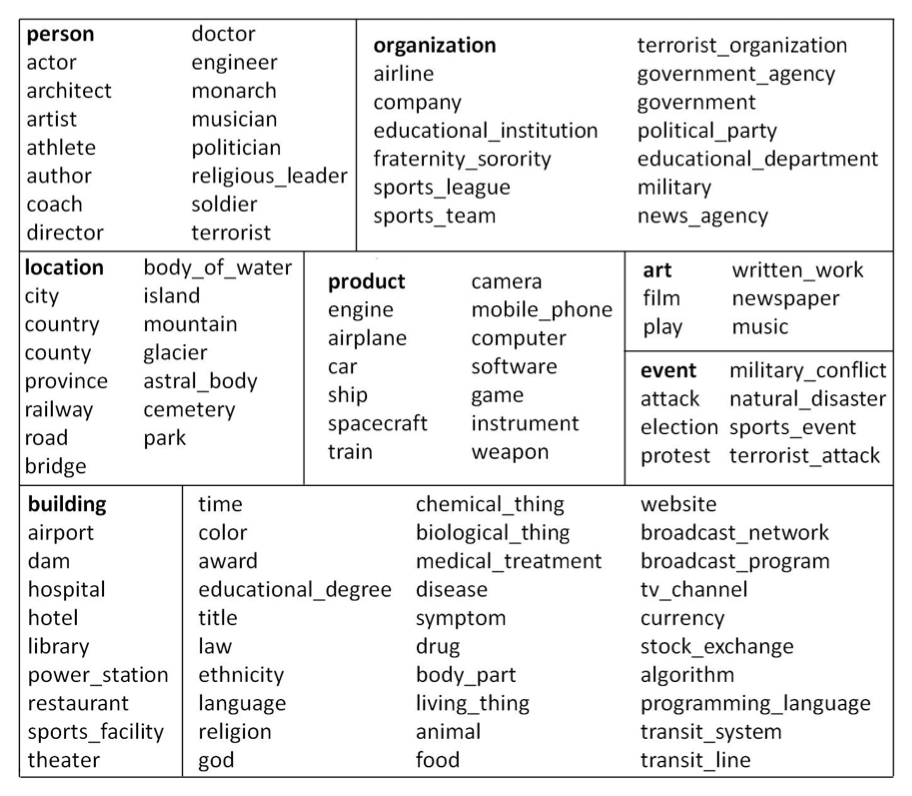
\includegraphics[width=0.7\linewidth]{figer.png}
    \caption{Type set of FIGER. Each box can be seen as a two-level tree, with the root node represented by the type in bold. The box at the bottom right is composed of uncategorized types. (Source:~\cite{Ling2012FineGrainedER})}
    \label{fig:figer}
\end{figure}

As said previously, the training set is obtained with a distant supervision technique and counts about $1.5M$ instances. The source of data that has been labeled is constituted by Wikipedia articles, where anchor links are treated as entity mentions. The annotation procedure can be summarized in three steps:
\begin{enumerate}
    \item For each sentence, detect all the linked segments $m$
    \item For each $m$, retrieve the related Wikipedia entity $e_{m}$
    \item For each $e_{m}$, obtain its types $t'_{m}$ from Freebase
    \item For each $t'_{m}$, refine the types to obtain a subset $t_{m} \subseteq t'_{m}$ such that $t_{m} \subseteq T$. The refinement is done by keeping only the ones with more than 5 ground instances and merging types that are too specific.
\end{enumerate}

The test set is composed of 434 manually annotated examples. The sentences are extracted from local newspapers, photography and veterinary magazines, and the student newspaper of the University of Washington.

Each entry of the dataset is represented following the structure of the JSON in Figure~\ref{fig:entry_bbn}. The main fields are \textit{tokens}, which contains the list of the worlds of the sentence, and \textit{mentions}. For each mention there are three subfields: \textit{start} and \textit{end} indicate the index of the tokens that delimits the mention, and \textit{labels} contains the true types.

\begin{figure}
    \centering
    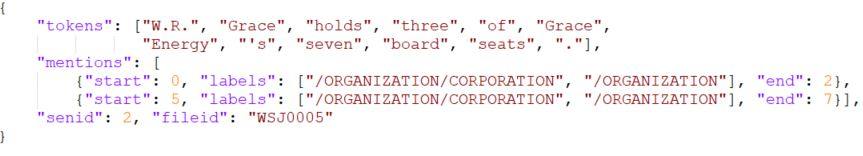
\includegraphics[width=1\linewidth]{figures/entry_bbn.JPG}
    \caption{Structure of a FIGER/BBN entry. Example taken from BBN.}
    \label{fig:entry_bbn}
\end{figure}

\subsubsection{BBN}
BBN dataset for FET made its first appearance in~\cite{ren2016noise} in 2016. The original version of this dataset comes from the BBN Pronoun Coreference and Entity Type Corpus~\cite{bbnCoreference}, composed of manually annotated Wall Street Journal articles. These articles were originally annotated using 93 types, divided into 12 named entity types, 9 nominal entity types, 7 numeric types, and 64 subtypes. However, when applying distant supervision, the authors used DBpedia Spotlight to link entities and they had to remove those BBN types that could not be mapped into Freebase types. The resulting type set counts 47 types.

The dataset is constituted by 32,739 entries. The test set has not been manually annotated. To construct it, the authors simply extracted a subset composed of the 20\% of the dataset,

An entry of the dataset is structured in the same way as FIGER (Figure~\ref{fig:entry_bbn}), so we can find the sentence as \textit{tokens} and the \textit{mentions} including \textit{start}, \textit{end} and \textit{labels} as subfields.

\subsubsection{Dataset preparation \& statistics} \label{dataset_stats}
The adopted versions of the datasets are those proposed by Ren et al. in~\cite{ren-etal-2016-afet}\footnote{https://github.com/INK-USC/AFET}. Before performing the experiments, both training sets of FIGER and BBN were refined. First of all, the duplicates (i.e., instances with the same context, mention, and types) were removed. Then, examples having the same context and different sets of mentions were merged. Each entry with more than one mention was subsequently divided into distinct entries with single mentions. Regarding FIGER, the equivalent types \texttt{/living\_thing} and \texttt{/livingthing} were unified in \texttt{/living\_thing}. Finally the sentences were split into 3 fields: \textit{left\_context\_token}, \textit{mention\_span} and \textit{right\_context\_token}. The mention types can be found in the field \textit{y\_str}. An example of an entry of the refined dataset is available in Figure~\ref{fig:entry_bbn_clean}. Since the dev sets were not provided within the original datasets, they were obtained by sampling about 1K instances of the training sets, such that single-mention examples derived from the same multi-mention example are assigned to the same set.

\begin{figure}
    \centering
    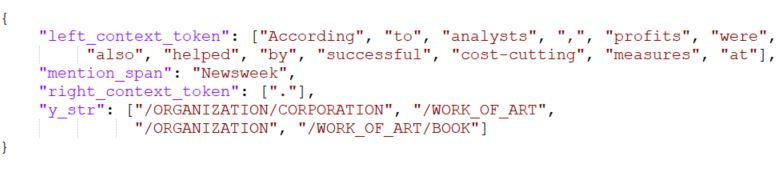
\includegraphics[width=1\linewidth]{figures/entry_bbn_clean.JPG}
    \caption{Structure of a FIGER/BBN entry after data preparation - Example taken from BBN}
    \label{fig:entry_bbn_clean}
\end{figure}

Before proceeding with the analysis of the datasets, it is helpful to point out that every sentence can contain multiple types from different branches. We will refer to this condition with the term multibranch. Furthermore, if an instance $x$ of the dataset is labeled with a type $t$ that is a subtype of $t'$, then the type set of $x$ must contain both $t$ and $t'$.

In Table~\ref{tab:dataset_stats} we can find some useful statistics about the two datasets. The fields of the table can be described as follows:
\begin{itemize}
    \item \textbf{\# ex:} number of examples of the refined version of the dataset
    \item \textbf{\% only supertype:} percentage of examples where a coarse type occurs without any of its subtypes
    \item \textbf{\% only supertype (strict):} percentage of examples where only coarse types occur
    \item \textbf{\% inter-tree:} percentage of examples where sibling types occur together
    \item \textbf{\% intra-tree:} percentage of examples where types from different trees occur together
    \item \textbf{\% intra/inter-tree:} percentage of examples where types from different branches occur together\footnote{this statistic is not equivalent to \textit{\%~inter-tree}~+~\%~intra-tree, since in the same example we could find both the situations}
    \item \textbf{\# types:} number of types of the refined version of the dataset
    \item \textbf{\# avg types:} average number of types per example
    \item \textbf{\% isolated types:} percentage of types corresponding to an isolated node\footnote{node without any parent or child} of the hierarchy
\end{itemize}

Looking at the table, it is possible to draw some considerations. In both datasets, we can observe that the multibranch examples are mostly caused by the presence of \textit{inter-tree} types. Regarding FIGER, we see that the statistics about \textit{only~supertype} are widely different between the training/dev and test sets. We have about the 21\% of cases against the 60\%, becoming 15\% against 54\% considering the \textit{strict} mode. This diversity derives from the manual annotation, where probably the types annotated through distant supervision that were too specific have been removed by the annotators. Even the statistics of \textit{intra/inter-tree} differ a lot between the training/dev and test sets. In this case, we move from the 35\% of multibranch examples to the 11\%. Again, the reason can be found in the manual annotation. Indeed, when using distant supervision techniques, a mention can be labeled with all its meanings disregarding the context. To point out how noisy is FIGER, we can also see how the \textit{\#~avg~types} statistic drastically decreases after the manual annotation.

Moving on to BBN, which does not have a manually annotated test set, the situation is quite different. First of all, we can notice that while the training/dev set counts the 22-24\% of multibranch examples, in the test set they are absent. This statistic is motivated by the fact that Ren et al. pruned these examples from the test set. For the same reason, we have no difference between the values of \textit{\%~only~supertype} and \textit{\%~only~supertype~(strict)} in the test. 

\begin{table}
\centering
\caption{Datasets statistics}
\label{tab:dataset_stats}
\resizebox{\columnwidth}{!}{\begin{tabular}{cccclll}
\hline
\multicolumn{1}{|c|}{\textbf{Dataset}} & \multicolumn{1}{c|}{\textbf{\# ex}}    & \multicolumn{1}{c|}{\textbf{\% only supertype}} & \multicolumn{1}{c|}{\textbf{\begin{tabular}[c]{@{}c@{}}\% only supertype\\ (strict)\end{tabular}}} & \multicolumn{1}{c|}{\textbf{\% inter-tree}} & \multicolumn{1}{c|}{\textbf{\% intra-tree}} & \multicolumn{1}{c|}{\textbf{\% inter/intra-tree}} \\ \hline
\multicolumn{1}{|c|}{BBN train}        & 84,492                                 & 16.0                                            & 7.64                                                                                               & \multicolumn{1}{c}{22.33}                   & \multicolumn{1}{c}{2.65}                    & \multicolumn{1}{c|}{24.09}                        \\
\multicolumn{1}{|c|}{BBN dev}          & 1,039                                  & 15.3                                            & 8.47                                                                                               & \multicolumn{1}{c}{20.69}                   & \multicolumn{1}{c}{2.31}                    & \multicolumn{1}{c|}{22.52}                        \\
\multicolumn{1}{|c|}{BBN test}         & 12,349                                 & 7.44                                            & 7.44                                                                                               & \multicolumn{1}{c}{-}                       & \multicolumn{1}{c}{-}                       & \multicolumn{1}{c|}{-}                            \\ \hline
\multicolumn{1}{|c|}{FIGER train}      & 2,676,854                              & 21.33                                           & 14.99                                                                                              & \multicolumn{1}{c}{23.63}                   & \multicolumn{1}{c}{15.38}                   & \multicolumn{1}{c|}{35.23}                        \\
\multicolumn{1}{|c|}{FIGER dev}        & 1,094                                  & 21.57                                           & 14.72                                                                                              & \multicolumn{1}{c}{25.59}                   & \multicolumn{1}{c}{14.35}                   & \multicolumn{1}{c|}{35.83}                        \\
\multicolumn{1}{|c|}{FIGER test}       & 563                                    & 60.57                                           & 54.17                                                                                              & \multicolumn{1}{c}{11.01}                   & \multicolumn{1}{c}{0.71}                    & \multicolumn{1}{c|}{11.72}                        \\ \hline
\multicolumn{1}{l}{}                   & \multicolumn{1}{l}{}                   & \multicolumn{1}{l}{}                            & \multicolumn{1}{l}{}                                                                               &                                             &                                             &                                                   \\ \cline{1-4}
\multicolumn{1}{|c|}{\textbf{Dataset}} & \multicolumn{1}{c|}{\textbf{\# types}} & \multicolumn{1}{c|}{\textbf{\# avg types}}      & \multicolumn{1}{c|}{\textbf{\% isolated types}}                                                    &                                             &                                             &                                                   \\ \cline{1-4}
\multicolumn{1}{|c|}{BBN train}        & 157,292                                & 1.86                                            & \multicolumn{1}{c|}{24.3}                                                                          &                                             &                                             &                                                   \\
\multicolumn{1}{|c|}{BBN dev}          & 1,903                                  & 1.83                                            & \multicolumn{1}{c|}{24.44}                                                                         &                                             &                                             &                                                   \\
\multicolumn{1}{|c|}{BBN test}         & 20,606                                 & 1.67                                            & \multicolumn{1}{c|}{15.4}                                                                          &                                             &                                             &                                                   \\ \cline{1-4}
\multicolumn{1}{|c|}{FIGER train}      & 6,380,532                              & 2.38                                            & \multicolumn{1}{c|}{9.21}                                                                          &                                             &                                             &                                                   \\
\multicolumn{1}{|c|}{FIGER dev}        & 2,616                                  & 2.39                                            & \multicolumn{1}{c|}{9.79}                                                                          &                                             &                                             &                                                   \\
\multicolumn{1}{|c|}{FIGER test}       & 840                                    & 1.49                                            & \multicolumn{1}{c|}{6.55}                                                                          &                                             &                                             &                                                   \\ \cline{1-4}
\end{tabular}}
\end{table}

The information about the hierarchy of each dataset are reported in Table~\ref{tab:dataset_hierarchy}. The columns of the table can be described as follows:
\begin{itemize}
    \item \textbf{\# nodes:} number of nodes of the hierarchy (i.e., cardinality of the type set)
    \item \textbf{\# levels:} maximum number of levels of a tree in the type set
    \item \textbf{\# top level:} number of root nodes with at least a child (i.e., supertypes)
    \item \textbf{\# leaves:} number of child nodes (i.e., subtypes)
    \item \textbf{\# isolated:} number of isolated nodes (i.e., neither supertypes nor subtypes)
\end{itemize}

\begin{table}
\centering
\caption{Datasets hierarchical structure}
\label{tab:dataset_hierarchy}
\begin{tabular}{|c|ccccc|}
\hline
\textbf{Dataset} & \multicolumn{1}{c|}{\textbf{\# nodes}} & \multicolumn{1}{c|}{\textbf{\# levels}} & \multicolumn{1}{c|}{\textbf{\# top level}} & \multicolumn{1}{c|}{\textbf{\# leaves}} & \textbf{\# isolated} \\ \hline
BBN              & 47                                     & 2                                       & 9                                          & 31                                      & 7                    \\ \hline
FIGER            & 128                                    & 2                                       & 22                                         & 79                                      & 27                   \\ \hline
\end{tabular}
\end{table}

\subsection{Baseline model} \label{baseline_model}
The architecture of the baseline network used in the experiments is shown in Figure~\ref{fig:et_baseline_architecture}. Starting from the input, the text is composed of three parts: left context (LC), mention (M), and right context (RC). The encoder receives a sequence in the form of \verb|[CLS]M[SEP]LC[SEP]RC|.  The example in the picture reports BERT as encoder, but any variant could be used to take its place. The versions used to perform the experiments of this thesis are BERT large\footnote{https://huggingface.co/bert-large-cased} and DistilBERT\footnote{https://huggingface.co/distilbert-base-uncased} for PyTorch\footnote{https://pytorch.org/}. In any case, the encoders are trained using the adapters with the Pfeiffer strategy. The framework used to integrate them into the models is AdapterHub\footnote{https://github.com/Adapter-Hub/adapter-transformers}. Once the encoder produces the output sequence, the encoding of the \verb|[CLS]| token is fed into a basic neural network composed of a fully connected layer and a classification layer. The fully connected layer has the same dimension as the encoder's output, the classification layer applies the sigmoid activation function to compute the probability to assign each label. Finally, there is the inference step to obtain the final predictions starting from the probabilities (more details in section~\ref{inference_rules}).

\begin{figure}[H]
    \centering
    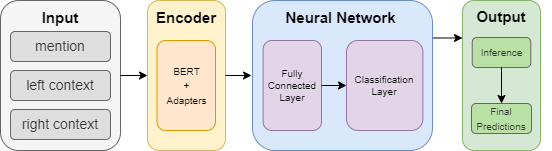
\includegraphics[width=.8\linewidth]{figures/et_baseline_architecture.png}
    \caption{Baseline model architecture}
    \label{fig:et_baseline_architecture}
\end{figure}


\subsection{KENN model} \label{kenn_model}
The architecture of the KENN-based model is designed starting from the baseline. As we can see in Figure~\ref{fig:et_kenn_architecture}, the architecture of the two models is almost the same. The only differences are the presence of KENN in the middle of the network and the KB provided to the model. The knowledge enhancement layer is placed between the fully connected layer and the classification layer. What said for the baseline model about input representation, encoders, etc. is still valid for this model.

\begin{figure}[H]
    \centering
    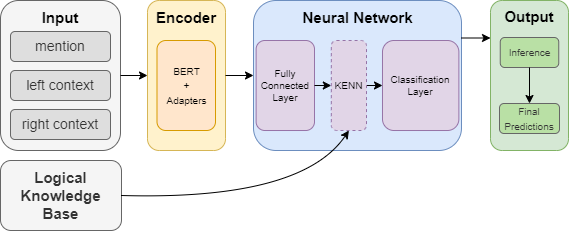
\includegraphics[width=.8\linewidth]{figures/et_kenn_architecture.png}
    \caption{KENN-based model architecture}
    \label{fig:et_kenn_architecture}
\end{figure}

Among the strategies for defining logical KB proposed in section~\ref{knowledge_generation}, the ones chosen for the experiments are the \textit{Bottom Up}, \textit{Top Down}, and \textit{Hybrid}. Other KB modes from Table~\ref{tab:kb_modes} are not taken into account since they do not apply to datasets with a 2-level hierarchy. We will not even analyze horizontal constraints since the priority has been given to the vertical ones. The number of clauses generated by the chosen KB modes are reported in Table~\ref{tab:dataset_clauses}.

\begin{table}
\centering
\caption{Datasets and number of clauses}
\label{tab:dataset_clauses}
\begin{tabular}{|c|ccc|}
\hline
\textbf{Dataset} & \multicolumn{1}{c|}{\textbf{Bottom Up}} & \multicolumn{1}{c|}{\textbf{Top Down}} & \textbf{Hybrid} \\ \hline
BBN              & 31                                      & 9                                      & 40              \\ \hline
FIGER            & 79                                      & 22                                     & 101             \\ \hline
\end{tabular}
\end{table}

Depending on the KB mode, KENN affects the predictions of the baseline network in different ways. Some statistics about the influence of the logical knowledge are available in Table~\ref{tab:dataset_stats_kenn}, which provides the following information:
\begin{itemize}
    \item \textbf{\% no clauses:} percentage of examples labeled with at least one type that does not occur in any clause (i.e. isolated type)
    \item \textbf{\% no clauses (strict):} percentage of examples labeled exclusively with types that do not occur in any clause (i.e. isolated types only)
    \item \textbf{\% inappropriate Top Down rules:} percentage of examples in which a supertype occurs without any of its subtypes; equivalent to \textit{\% only supertype} in Table~\ref{tab:dataset_stats}
    \item \textbf{\% inappropriate Top Down rules (strict):} percentage of examples in which only supertypes occur; equivalent to \textit{\% only supertype (strict)} in Table~\ref{tab:dataset_stats}
\end{itemize}
With the term \textit{``inappropriate"} used in the last two statistics, we mean that the intervention of KENN may be undesired. Contrarily to what happens in Bottom Up, the knowledge enhancement could be disadvantageous when using the Top Down mode in some cases. The reason is that a Top Down clause will always encourage the model to predict subtypes even when the ground truth contains only supertypes. Indeed, we saw in section~\ref{knowledge_generation} that while Bottom Up respects the Open World Assumption, Top Down is defined under the Closed World Assumption. About the statistics from the table, we can notice relevant differences between the train/dev and the test sets. The most evident one regards FIGER and the \textit{Top Down} statistics, where we can observe a difference of 40 percentage points.


\begin{table}
\centering
\caption{Datasets statistics on KENN's influence}
\label{tab:dataset_stats_kenn}
\resizebox{\columnwidth}{!}{\begin{tabular}{|c|cccc|}
\hline
\textbf{Dataset} & \multicolumn{1}{c|}{\textbf{\% no clauses}} & \multicolumn{1}{c|}{\textbf{\begin{tabular}[c]{@{}c@{}}\% no clauses\\ (strict)\end{tabular}}} & \multicolumn{1}{c|}{\textbf{\begin{tabular}[c]{@{}c@{}}\% inappropriate\\ Top Down rules\end{tabular}}} & \textbf{\begin{tabular}[c]{@{}c@{}}\% inappropriate\\ Top Down rules\\ (strict)\end{tabular}} \\ \hline
BBN train        & 44.74                                       & 37.01                                                                                          & 16.00                                                                                                   & 7.64                                                                                          \\
BBN dev          & 44.47                                       & 37.05                                                                                          & 15.30                                                                                                   & 8.47                                                                                          \\
BBN test         & 25.69                                       & 25.69                                                                                          & 7.44                                                                                                    & 7.44                                                                                          \\ \hline
FIGER train      & 18.06                                       & 9.85                                                                                           & 21.33                                                                                                   & 14.99                                                                                         \\
FIGER dev        & 20.02                                       & 10.79                                                                                          & 21.57                                                                                                   & 14.72                                                                                         \\
FIGER test       & 9.59                                        & 5.33                                                                                           & 60.57                                                                                                   & 54.17                                                                                         \\ \hline
\end{tabular}}
\end{table}

\subsection{Inference rules} \label{inference_rules}
The scores produced by the model can be processed through different inference rules to transform the probability of each class into a binary prediction. The most common strategy to discriminate between positive and negative predictions in classification problems is to use a threshold, but there are many alternatives that may lead to better results. The choice of the inference rule may heavily affect the evaluation of a model. Given an instance, we indicate with $Y$ the set of output values of the neural network and with $y$ the output for a specific type. The inference rules that will be used to compute the final predictions are the following:
\begin{enumerate}
    \item \textbf{Threshold:} basic inference method which simply compare the scores with the threshold
    \begin{gather*}
        pred(y) = 1 \iff score(y) > threshold
    \end{gather*}
    \item \textbf{Threshold or max:} same as \textit{threshold}'s method, but it prevents void predictions by assigning the class with maximum score when none of the scores exceeds the threshold
    \begin{gather*}
        pred(y) = 1 \iff (score(y) > threshold \vee score(y) = \max_{y_{i}\in Y}score(y_{i}))
    \end{gather*}
    This inference rule is commonly used by FET from the literature.
\end{enumerate}
\section{Experiments} \label{experiments}
The conducted experiments involve many parameters that can be varied and combined to observe KENN's behavior from several points of view. The space of parameters is the following:
\begin{itemize}
    \item \textbf{KB mode:} the KB encoding strategy used to define the logical knowledge
    \item \textbf{initial clause weight:} the value used to initialize the network parameters of the clause weights
    \item \textbf{fixed/learnable clause weights:} the strategy used to set the clause weights
    \item \textbf{encoder:} the language model used to encode the textual input
    \item \textbf{loss function:} the loss function used during training
\end{itemize}
Before describing the experiments, we will introduce in the next sections the ET metrics and the training setups adopted. It is also important to point out that every model used the same initialization of random seeds, which guarantees: 
\begin{enumerate}
    \item Same layer initialization between different setups
    \item Given an epoch, each model is trained on the same batch of data
\end{enumerate}



\subsection{Metrics for Entity Typing}
The evaluation of an ET approach relies on some variants of the metrics used in classical classification problems. The explanation of each metric will be supported by numerical values obtained from the example in Table~\ref{tab:metrics_example}. 

\begin{table}[H]
\centering
\caption{Example of predictions over a type set $T=\{T1, T2, T3\}$ and a dataset $X=\{X1, X2, X3\}$}
\label{tab:metrics_example}
\begin{tabular}{c|ccc|ccc|}
\cline{2-7}
                                       & \multicolumn{3}{c|}{\textbf{Prediction}}                                          & \multicolumn{3}{c|}{\textbf{Target}}                                              \\ \hline
\multicolumn{1}{|c|}{\textbf{Example}} & \multicolumn{1}{c|}{\textbf{T1}} & \multicolumn{1}{c|}{\textbf{T2}} & \textbf{T3} & \multicolumn{1}{c|}{\textbf{T1}} & \multicolumn{1}{c|}{\textbf{T2}} & \textbf{T3} \\ \hline
\multicolumn{1}{|c|}{X$_{1}$}          & x                                &                                  & x           & x                                & x                                &             \\ \hline
\multicolumn{1}{|c|}{X$_{2}$}          &                                  & x                                &             & x                                &                                  & x           \\ \hline
\multicolumn{1}{|c|}{X$_{3}$}          & x                                &                                  & x           & x                                &                                  & x           \\ \hline
\end{tabular}
\end{table}

In the definition of the metrics we will use terminology that needs a preliminary explanation:
\begin{itemize}
    \item True Positive (\textbf{TP}): number of correct positive predictions. In the example in Table~\ref{tab:metrics_example} we have TP=3 .
    \item False Positive (\textbf{FP}): number of wrong positive predictions. In the example in Table~\ref{tab:metrics_example} we have FP=2 .
    \item True Negative (\textbf{TN}): number of correct negative predictions. In the example in Table~\ref{tab:metrics_example} we have TN=1 .
    \item False Negative (\textbf{FN}): number of wrong negative predictions. In the example in Table~\ref{tab:metrics_example} we have FN=3 .
\end{itemize}

Once fixed these preliminary notions, the evaluated metrics are defined as follows:

\begin{itemize}
    \item \textbf{Accuracy:} percentage of correct predictions; defined as 
    \begin{gather*}
        \frac{count(Prediction == Target)}{|X|} = \frac{1}{3}
    \end{gather*}
    
    \item \textbf{Micro precision:} percentage of correct positive predictions with respect to all the positive predictions; defined as
    \begin{gather*}
        \frac{TP}{TP + FP} = \frac{3}{3 + 2} = 0.6
    \end{gather*}
    
    \item \textbf{Micro recall:} percentage of correct positive predictions with respect to the positive target; defined as
    \begin{gather*}
        \frac{TP}{TP + FN} = \frac{3}{3 + 3} = 0.5
    \end{gather*}
    
    \item \textbf{Micro f1:} harmonic mean of micro precision and micro recall; defined as
    \begin{gather*}
        2 \cdot \frac{MicroPrecision \cdot MicroRecall}{MicroPrecision + MicroRecall} =
        2 \cdot \frac{0.6 \cdot 0.5}{0.6 + 0.5} = 0.54
    \end{gather*}
    
    \item \textbf{Macro precision examples:} mean of the percentages of correct positive predictions with respect to all the positive predictions of each example; defined as
    \begin{gather*}
        \frac{\sum_{x \in X}\frac{TP(x)}{TP(x) + FP(x)}}{|X|}=
        \frac{0.5 + 0 + 1}{3}=0.5
    \end{gather*}
    
    \item \textbf{Macro recall examples:} mean of the percentages of correct positive predictions with respect to the positive target of each example; defined as
    \begin{gather*}
        \frac{\sum_{x \in X}\frac{TP(x)}{TP(x) + FN(x)}}{|X|}=
        \frac{0.5 + 0 + 1}{3}=0.5
    \end{gather*}
    
    \item \textbf{Macro f1 examples:} harmonic mean of micro precision examples and micro recall examples; defined as
    \begin{gather*}
        2 \cdot \frac{MacroPrecisionExamples \cdot MacroRecallExamples}{MacroPrecisionExamples + MacroRecallExamples} =\\
        = 2 \cdot \frac{0.5 \cdot 0.5}{0.5 + 0.5} = 0.5
    \end{gather*}
    
    \item \textbf{Macro precision classes:} mean of the percentages of correct positive predictions with respect to all the positive predictions of each class; defined as
    \begin{gather*}
        \frac{\sum_{t \in T}\frac{TP(t)}{TP(t) + FP(t)}}{|T|} =
        \frac{1 + 0 + 0.5}{3} = 0.5
    \end{gather*}
    
    \item \textbf{Macro recall classes:} mean of the percentages of correct positive predictions with respect to the positive target of each class; defined as
    \begin{gather*}
        \frac{\sum_{t \in T}\frac{TP(t)}{TP(t) + FN(t)}}{|T|} =
        \frac{0.66 + 0 + 0.5}{3} = 0.38
    \end{gather*}
    
    \item \textbf{Macro f1 classes:} harmonic mean of macro precision classes and macro recall classes; defined as
    \begin{gather*}
        2 \cdot \frac{MacroPrecisionClasses \cdot MacroRecallClasses}{MacroPrecisionClasses + MacroRecallClasses} = \\
        = 2 \cdot \frac{0.5 \cdot 0.38}{0.5 + 0.38} = 0.43
    \end{gather*}
\end{itemize}
% \pagebreak
\subsection{Experimental setups}
Two setups were adopted for the experiments. The main differences between the setups are the stopping criterion and the batch size. In particular, \textit{Setup B} is used when BERT is involved since \textit{Setup A} would be too expensive.
\paragraph{Setup A} 
\begin{itemize}
    \item \textbf{number of epochs:} 100 for FIGER, 75 for BBN\footnote{BBN is smaller than FIGER and converges faster}
    \item \textbf{number of examples per epoch:} 10,240 (20 batches\footnote{using $n$ batches per epoch means performing $n$ backward operations per epoch} of size 512)
    \item \textbf{data shuffle:} each time the whole dataset has been seen
    \item \textbf{optimizer:} Adam with fixed learning rate set to 0.0005
    \item \textbf{inference:} threshold = 0.5
\end{itemize}

\paragraph{Setup B} 
\begin{itemize}
    \item \textbf{number of epochs:} undefined; determined by an early stopping strategy on the \textit{dev loss} with \textit{patience = 5}
    \item \textbf{number of examples per epoch:} 10,240 (160 batches of size 64)
    \item \textbf{data shuffle:} every time the whole dataset has been seen
    \item \textbf{optimizer:} Adam with fixed learning rate set to 0.0005
     \item \textbf{inference:} threshold = 0.5
\end{itemize}


\subsection{Baseline hyperparameter search}
The architecture of the baseline neural network was kept simple to have a basic starting point, so it did not involve any search of the best combination of hidden layers/units. The optimization aimed to find the best representation of the input text in terms of tokens and involved a few hyperparameters.


Fixed the training configuration following the \textit{Setup A}, we can proceed with the explanation of the hyperparameter search. We saw in section \ref{baseline_model} that the input of the model is split in mention, left context and right context tokens separated by \verb|[SEP]|. Although keeping every token of every span would feed the model with the maximum amount of information, this is not a feasible solution because of the high cost. For this reason, it is necessary to find the optimal number of tokens for both mention and context to reach a trade-off between cost and performance. Before going on, an important remark: tokens and words are two distinct things. In this case, we are looking for the optimal number of words that will be transformed by the tokenizer into a different number of tokens. Since BERT's tokenization is based on the WordPiece, the number of tokens grows up rapidly due to the subwords segmentation. For this reason, the maximum number of tokens is capped to 80 (left-to-right) for not exceeding the resource usage. Sequences with less than 80 tokens are filled with empty tokens.

The optimization is based on the metrics of \textit{macro f1 examples} and \textit{macro f1 classes} in this order of relevance. The search is performed iteratively by changing the number of words to keep for each input part. Starting from 1 mention word without any context, the number of mention words is increased until it stops improving. Once fixed the length of the mention, the left and right contexts get increased until reaching convergence. The two contexts share the same length.
\\\\
The best configurations found for the two datasets are the following:
\begin{itemize}
    \item \textbf{FIGER:} \texttt{mention = 6}, \texttt{context = 19}
    \item \textbf{BBN:} \texttt{mention = 5}, \texttt{context = 13}
\end{itemize}
Since these parameters refer to DistilBERT, the search procedure should be repeated for BERT to use it at its best. However, this has not been done for cost reasons. Aware of this, the same parameters have been used for both the encoders.
\subsection{Initial experiments with KENN}
The goal of these experiments is to analyze how KENN behaves when involved in a FET task. When the framework has been introduced in section \ref{KENN}, we saw that it allows using different settings about clause weights (i.e., fixed values, learnable parameters). However, the best choice for this context needs to be discovered. The same goes for the KB modes, as several alternatives were proposed without knowing which one would be the most promising for our task. Given these premises, the analysis can be divided into two parts. The first part is constituted by some \textit{quantitative analysis} (section~\ref{quantitative_analysis}) and aims to study the impact of each configuration of KENN. The second part is called \textit{preactivations analysis} (section~\ref{preactivation_analysis}) and investigates what happens in the network at a lower level.

\subsubsection{Setup}
Both the baseline and KENN-based models used in these experiments follow the \textit{Setup A}. The tested configurations are obtained with the following parameters:
\begin{itemize}
    \item \textbf{KB modes:} Bottom Up, Top Down and Hybrid
    \item \textbf{initial clause weights:} 0.5, 1.0 and 2.0
    \item \textbf{fixed clause weights}
    \item \textbf{encoder:} DistilBERT with adapters
    \item \textbf{loss function:} Binary Cross-Entropy, with the weights of positive examples set to 1
\end{itemize}
Each KB mode is tested by varying the initial clause weight, counting a total of 9 KENN's configurations. Clause weights are set as non-learnable parameters to force KENN to treat them all equally during the enhancement process and to ensure the presence of KENN for all the training.

\subsubsection{Terminology}
The following terminology will be used during the analysis:
\begin{itemize}
    \item \textbf{F:} stands for \textit{Father} (i.e, supertype); used to indicate a type that corresponds to a father node in the hierarchical tree
    \item \textbf{S:} stands for \textit{Son} (i.e., subtype); used to indicate a type that corresponds to a child node in the hierarchical tree
    \item \textbf{pre-KENN state:} values of the preactivations provided to KENN as input
    \item \textbf{post-KENN state:} values of the preactivations after KENN (i.e., final output)
\end{itemize}
\textit{\textbf{Additional note:} in some circumstances we may say that the baseline model and the pre-KENN network are equivalent. To avoid misunderstanding, the term ``equivalent" is intended as identical architecture and initialization, excluding KENN's layer.}


\subsubsection{Quantitative analysis} \label{quantitative_analysis}
This is a high-level analysis based on the performance obtained by the models on the dev set during the training process. The involved studies will try to answer the following questions:
\begin{enumerate}
    \item \textbf{Effects of different clause weights:} how much does the weight of a clause affect the final predictions?
    \item \textbf{Effects of each KB mode:} is there a winning strategy to define clauses that brings more benefits than the others? does the winning strategy perform better than the baseline?
    \item \textbf{Metrics per type:} is there a KB mode that enhances the performance on certain types?
\end{enumerate}

\subsubsection{Preactivations analysis} \label{preactivation_analysis}
The preactivations produced by the models are the core of this analysis. Since the pre-KENN network and the baseline model share the same architecture and initialization, these studies aim to analyze how the networks evolve differently seeing the same data. Furthermore, for each KB mode, we will study how the types F and S involved in the same clause influence each other. The study can be divided into the following analysis:
\begin{enumerate}
    \item \textbf{Distributions analysis:} it compares the distributions of the pre-KENN, post-KENN, and baseline preactivations.
    \item \textbf{Finite State Machines (FSM) analysis:} it studies the effects of each KB mode with respect to the preactivations of the types F and S involved in the same clause. FSMs are a compact and intuitive way to represent the available transitions between pre-KENN and post-KENN states accordingly to the KB mode.
    \item \textbf{Sankey diagrams\footnote{a Sankey diagram is a flow diagram where the width of the arrows represents the flow rate between two states} analysis:} it supports the FSM analysis by adding information about the number of examples involved in each transition. 
\end{enumerate}
The FSM analysis needs the introduction of a clear notation. In Figure~\ref{fig:fsm_example} we can find an example of FSM with random transitions. The terminology used is quite simple:
\begin{itemize}
    \item \textbf{FxSy}: arbitrary state where $ F = x $ and $ S = y $, with $x,y \in \{0, 1\}$; F and S are types involved in the same clause
    \item \textbf{F*S*$\to$F*S*:} transition from a pre-KENN state to a post-KENN state
    \item \textbf{forbidden state:} F0S1 (circled in red); this state should never occur as final state since it represents a violation of the hierarchy
    \item \textbf{p(F*S*$\to$F*S*):} probability to move from a pre-KENN state to a post-KENN state
    \item \textbf{\% correct:} percentage of transitions from a wrong\footnote{wrong = at least one between F and S is wrongly predicted} pre-KENN state to a correct\footnote{correct = both F and S are correctly predicted} post-KENN state
    \item \textbf{\% wrong:} percentage of transitions from a correct pre-KENN state to a wrong post-KENN state
    \item \textbf{\% other:} percentage of transitions from a wrong pre-KENN state to a wrong post-KENN state
\end{itemize}
\begin{figure}[H]
    \centering
    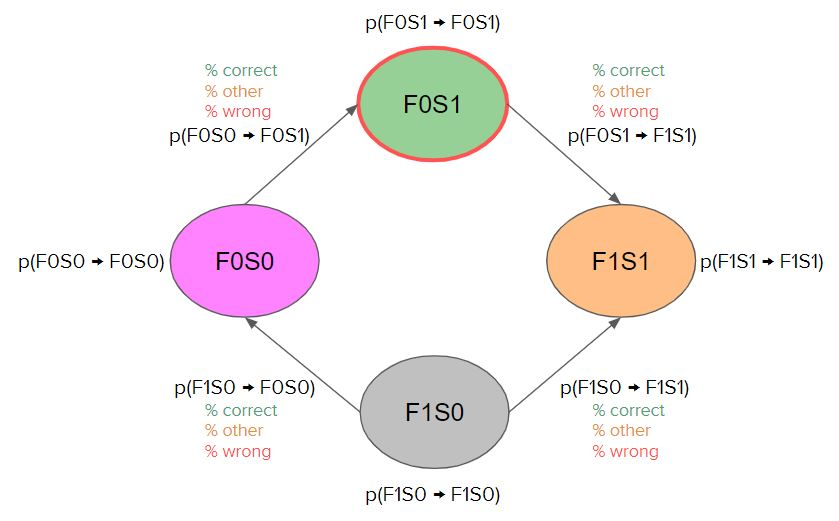
\includegraphics[width=.8\linewidth]{figures/fsm_example.jpg}
    \caption{ Example of a Finite State Machine }
    \label{fig:fsm_example}
\end{figure}
A few final notes on the FSM representation:
\begin{itemize}
    \item probabilities and percentages are extracted from the dev set
    \item self loop transitions are omitted from the graphical representation
    \item the sum of probababilities of outgoing transitions, including self loops, must be equal to 1
\end{itemize}

\subsubsection{Results on FIGER}
Only for these experiments, a reduced version of FIGER is used with the purpose to anticipate training convergence. The subset of the dataset is extracted by a random sample that counts approximately 267K training examples.
\paragraphn{Quantitative analysis 1 - Clause weights}
The performance in terms of \textit{macro f1 examples} obtained by varying the initial clause weights is available in Figure~\ref{fig:wandb_weights_comparison}. Looking at the graphs, we can observe a common behavior: regardless of the KB mode, the influence of different weights is visible only in the first 15-20 epochs (i.e., the red line in the graph is above the others in the initial epochs). Especially for the Hybrid mode, we can see in Figure~\ref{fig:wandb_weights_comparison_h} how the largest weight gives a clear initial boost to the performance. However, the boost tends to diminish over the epochs until it disappears. Another interesting behavior can be found in Figure~\ref{fig:wandb_weights_avg_pred_start}, which shows the evolution of the \textit{average predictions number} in the first 20 epochs. From the figures, we can observe that the larger the weight, the higher the number of predictions, and the larger the weight, the higher the performance. We can deduce from these results that the increased performance is due to an increased number of correct predictions, otherwise we would not see an increment in the performance. To conclude, we can say that a major influence of KENN helps the network to learn faster when it has not yet seen a big amount of training examples.
\\\\
\textit{\textbf{Note:} the previous considerations still apply to the other metrics not reported here}

\begin{figure}
     \centering
     \begin{subfigure}{0.8\textwidth}
         \centering
         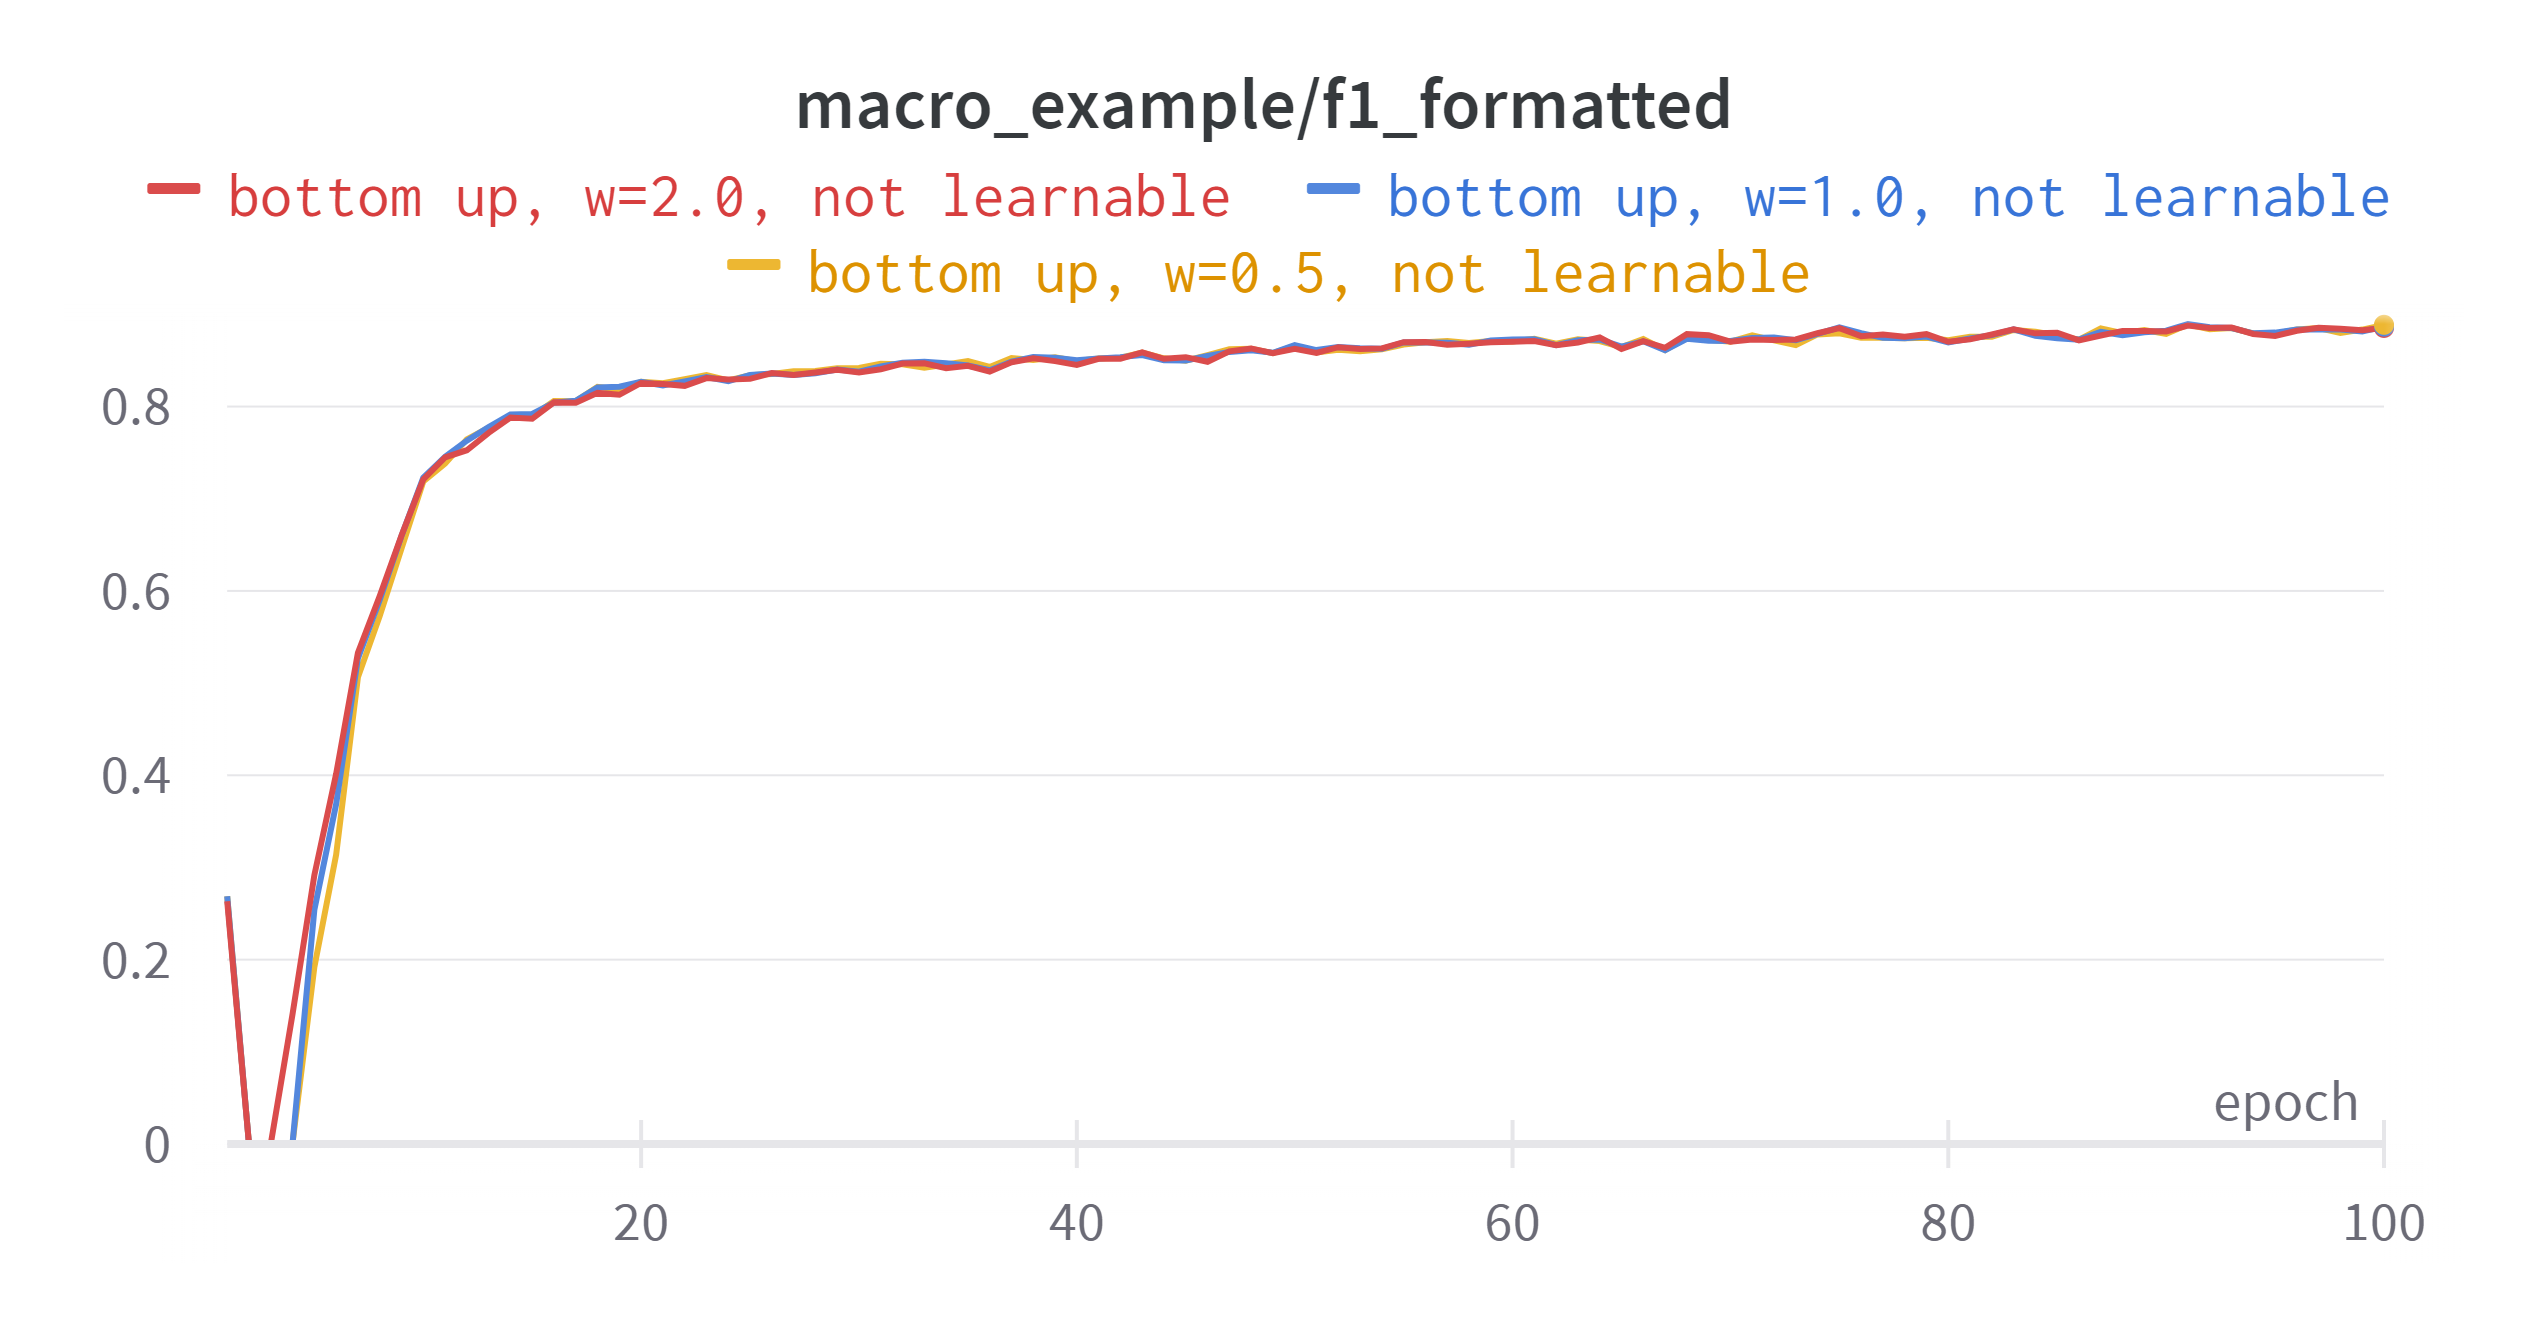
\includegraphics[width=\textwidth]{figures/wandb_weights_bottom_up_macro_ex_f1.png}
         \caption{Bottom Up}
     \end{subfigure}
     \vfill
     \begin{subfigure}{0.8\textwidth}
         \centering
         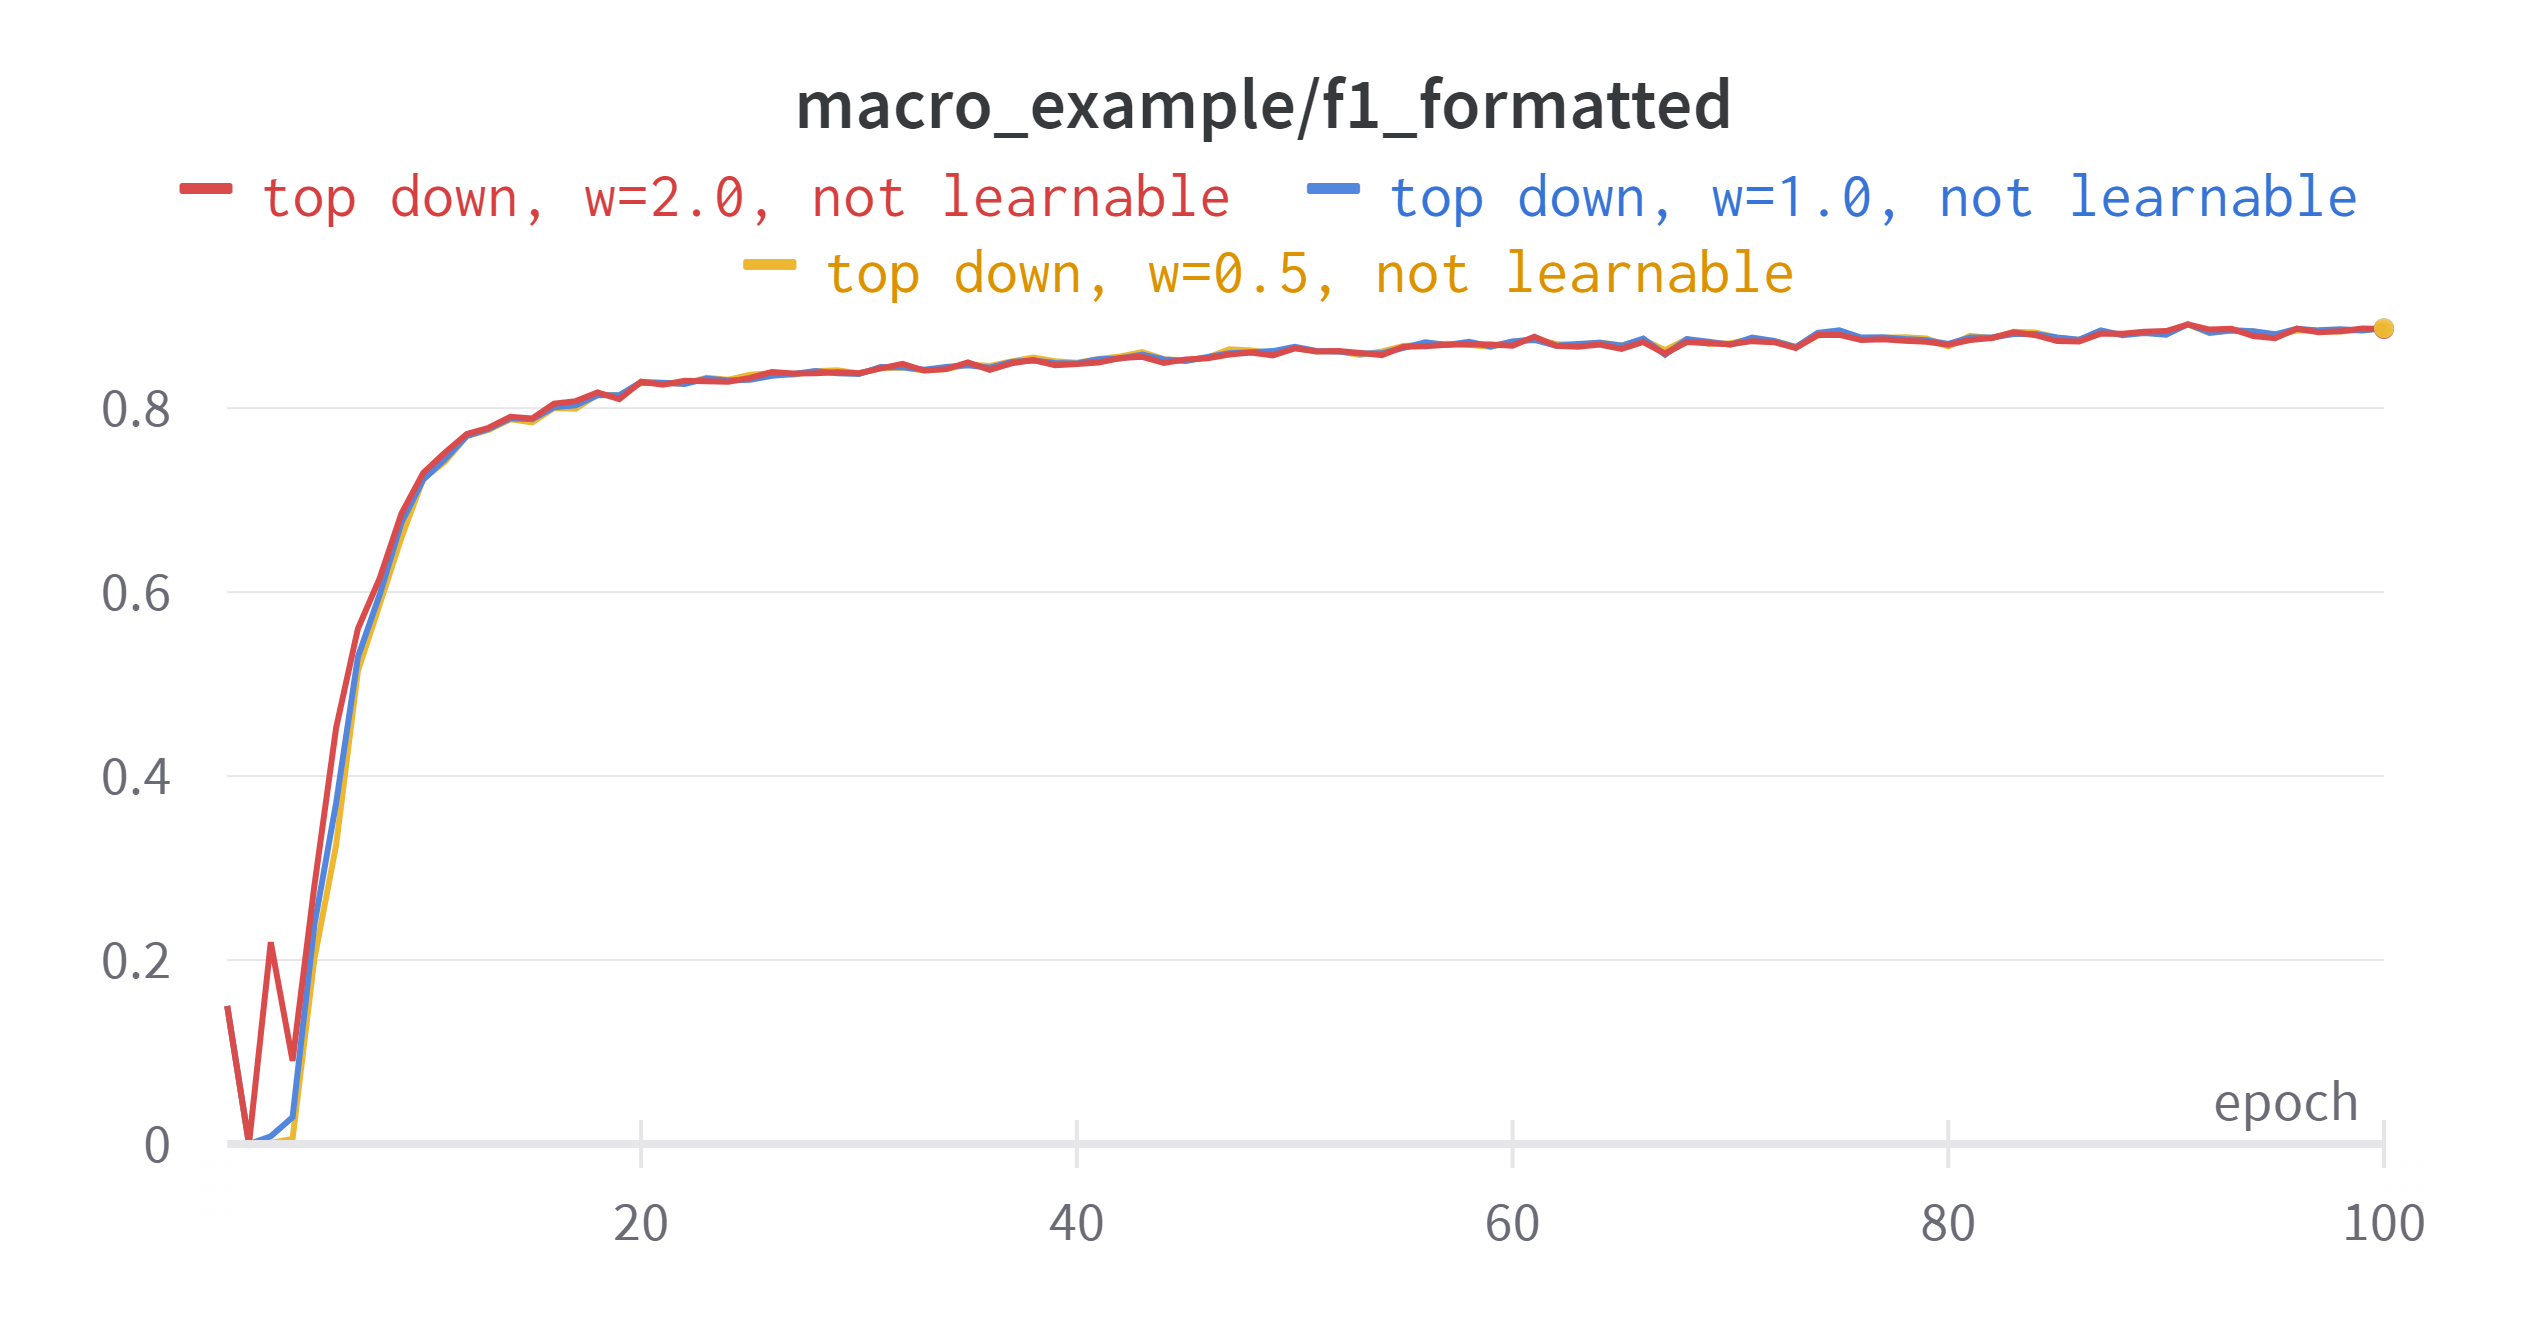
\includegraphics[width=\textwidth]{figures/wandb_weights_top_down_macro_ex_f1.png}
         \caption{Top Down}
     \end{subfigure}
     \vfill
     \begin{subfigure}{0.8\textwidth}
         \centering
         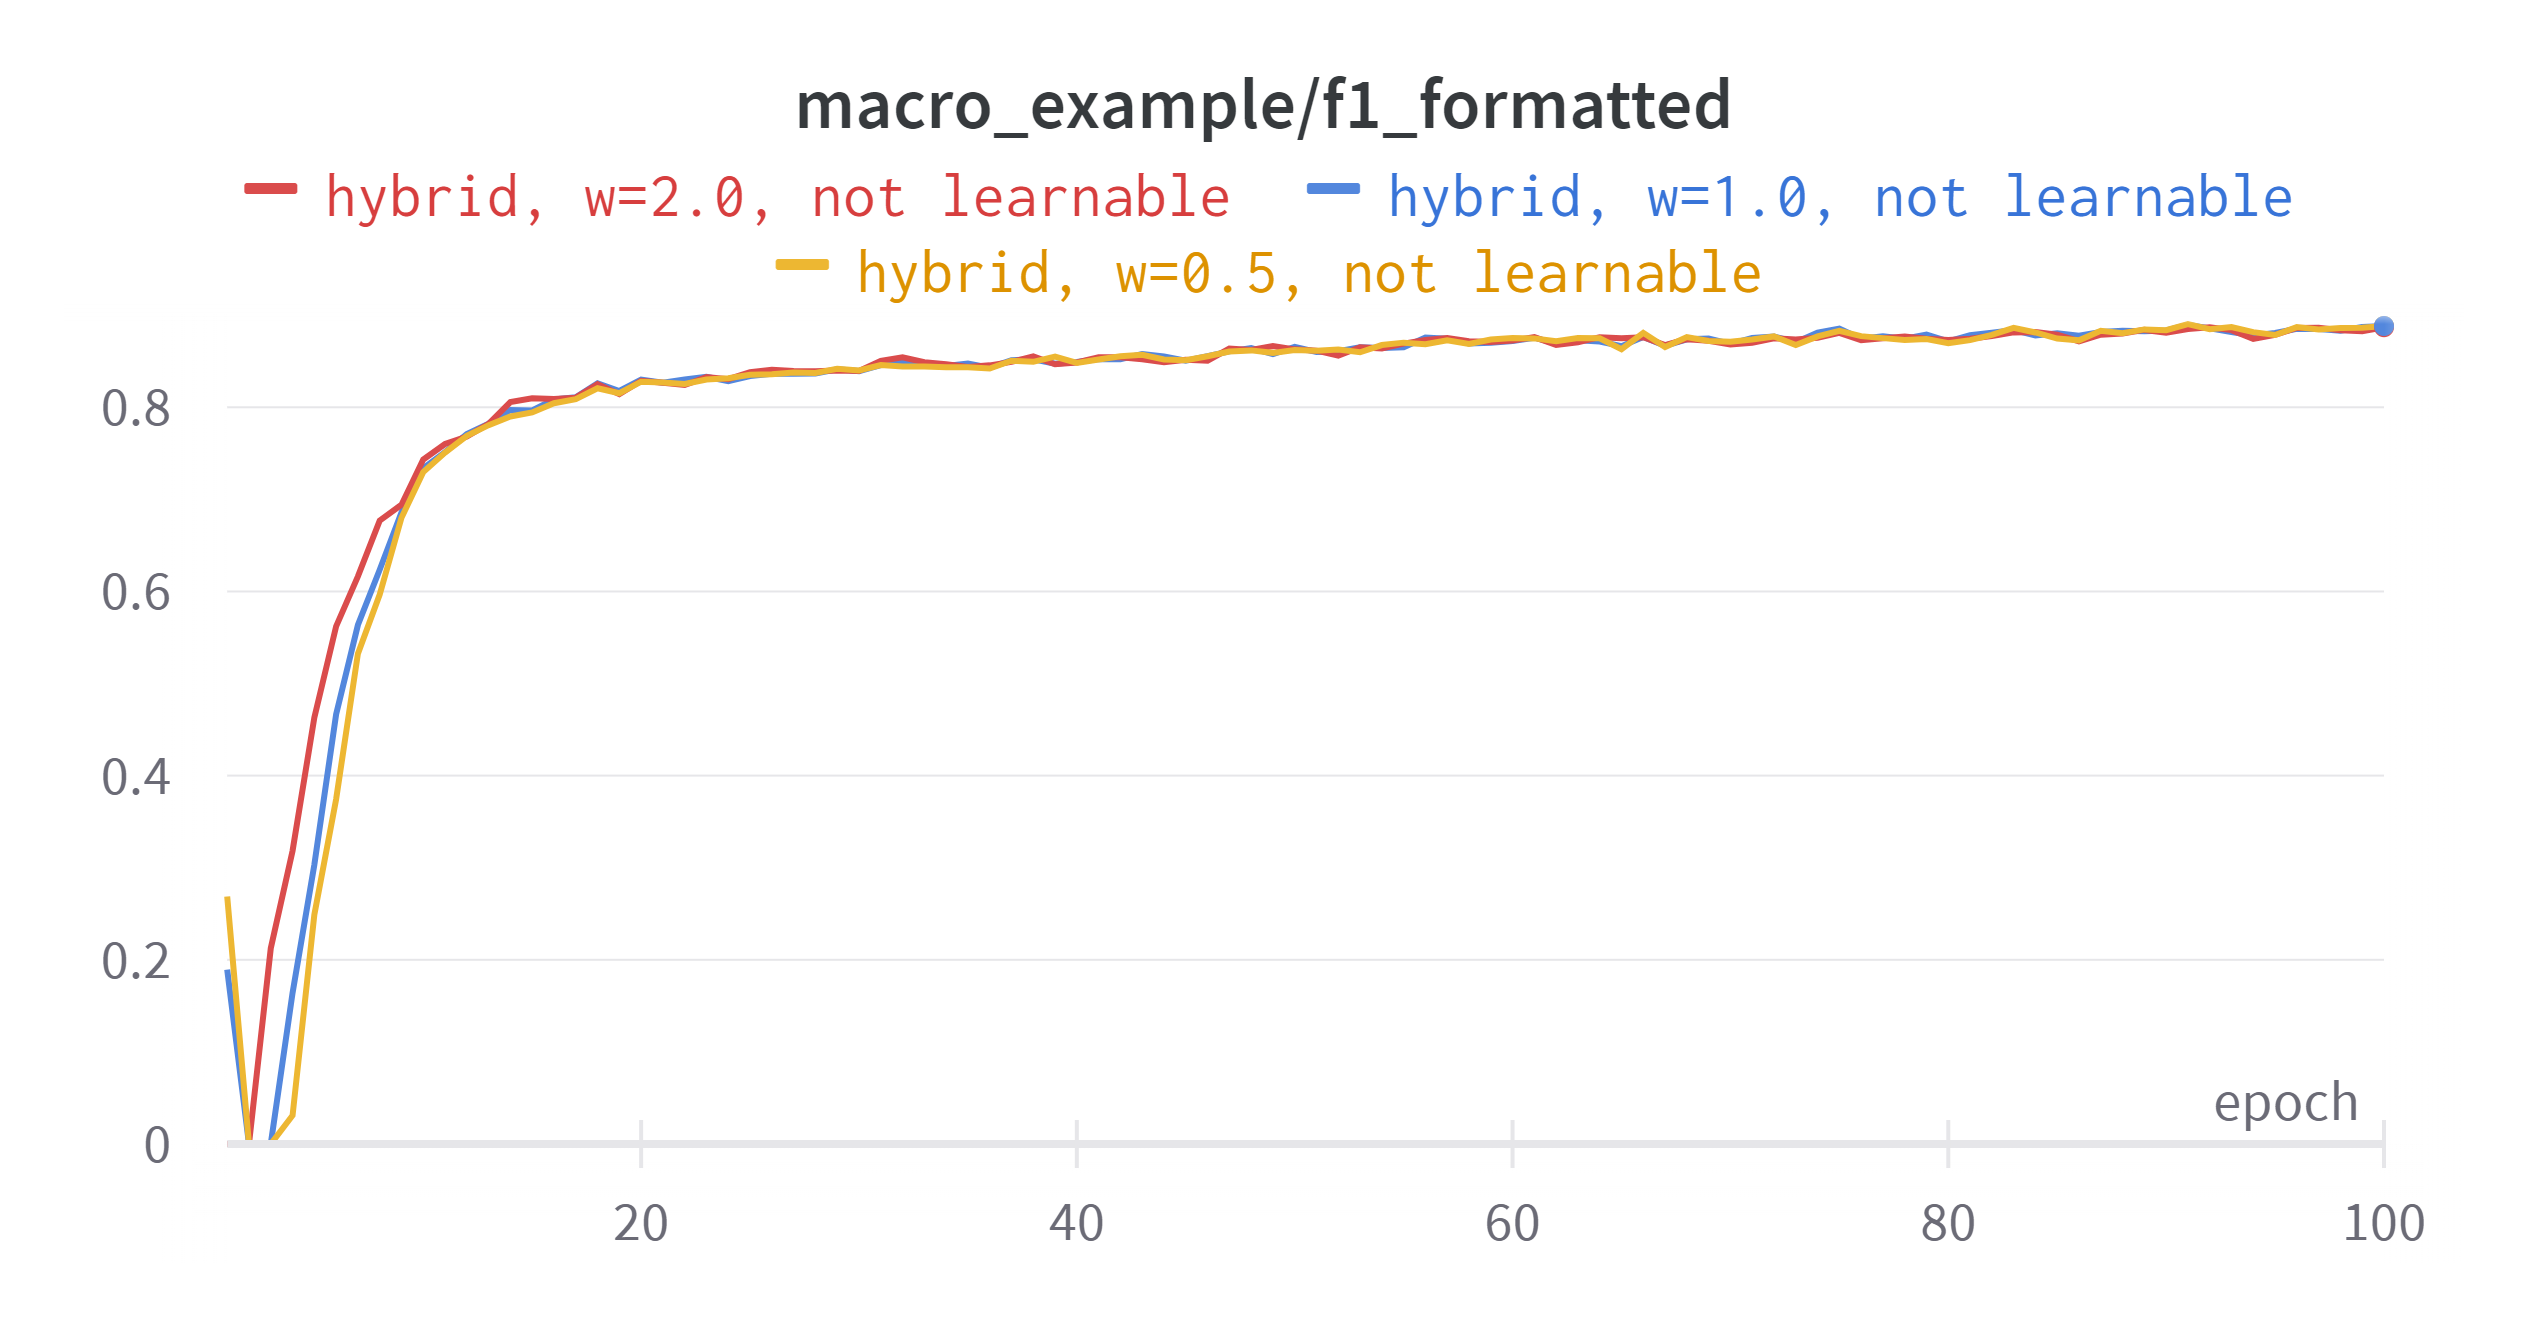
\includegraphics[width=\textwidth]{figures/wandb_weights_hybrid_macro_ex_f1.png}
         \caption{Hybrid}
         \label{fig:wandb_weights_comparison_h}
    \end{subfigure}
        \caption{Comparison of \textit{macro f1 examples} by varying the clause weight for each KB mode, with DistilBERT-based models evaluated on the dev set of FIGER.}
        \label{fig:wandb_weights_comparison}
\end{figure}

\begin{figure}
     \centering
     \begin{subfigure}{0.8\textwidth}
         \centering
         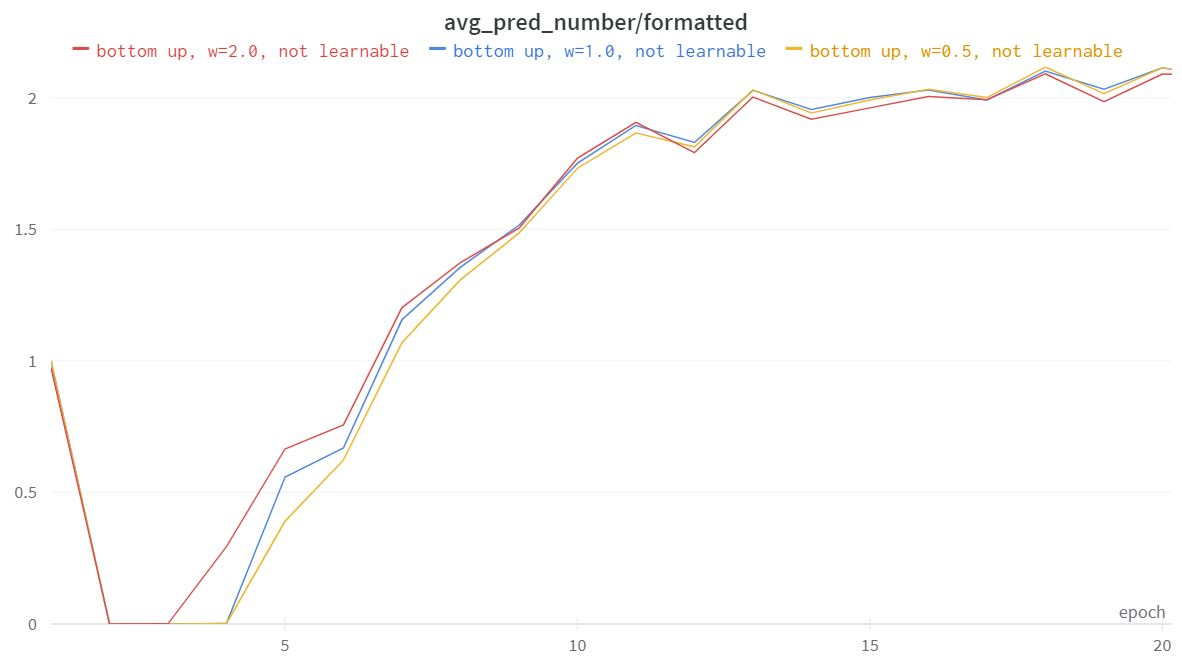
\includegraphics[width=\textwidth]{figures/wandb_weights_bottom_up_avg_pred_start.JPG}
         \caption{Bottom Up}
     \end{subfigure}
     \vfill
     \begin{subfigure}{0.8\textwidth}
         \centering
         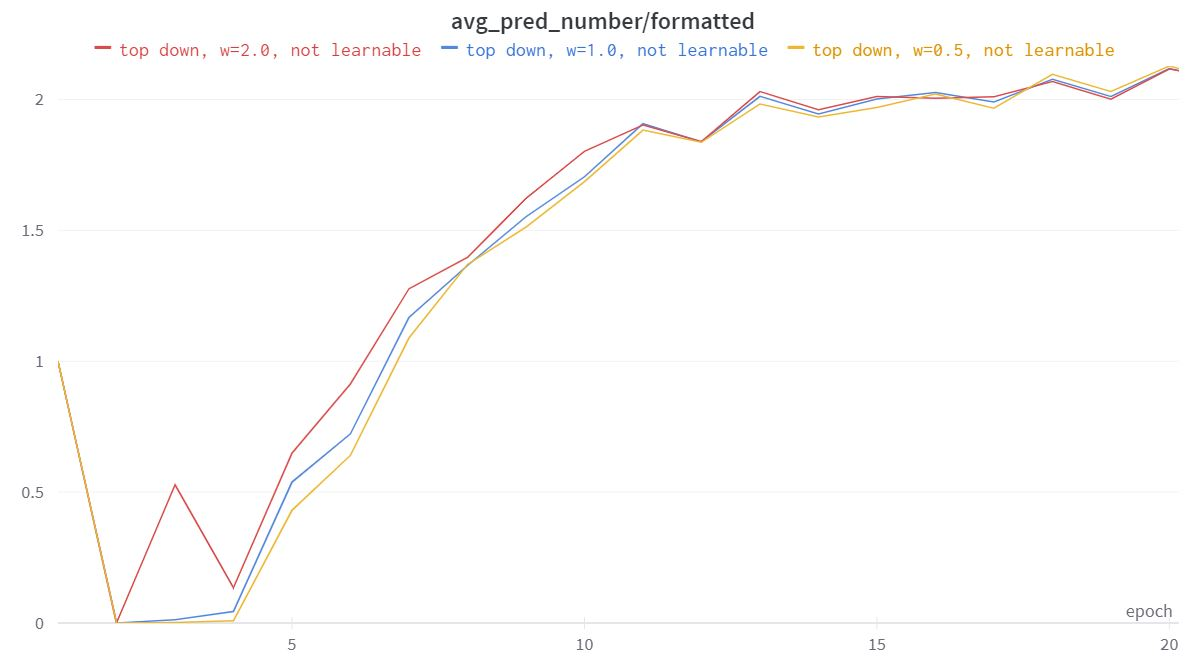
\includegraphics[width=\textwidth]{figures/wandb_weights_top_down_avg_pred_start.JPG}
         \caption{Top Down}
     \end{subfigure}
     \vfill
     \begin{subfigure}{0.8\textwidth}
         \centering
         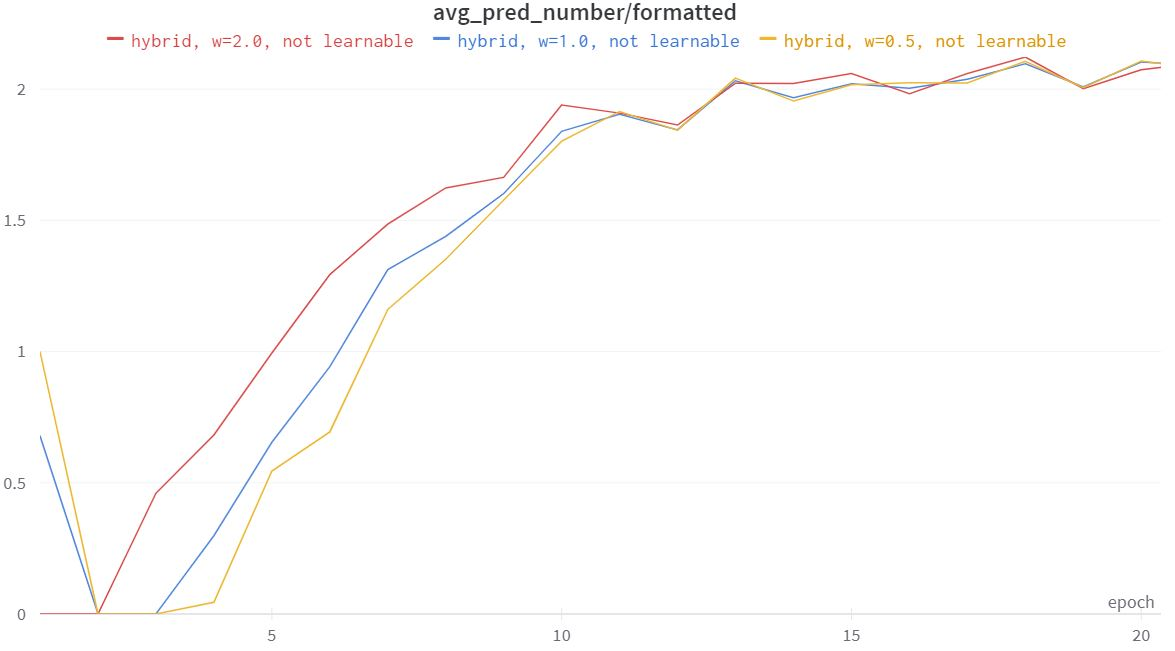
\includegraphics[width=\textwidth]{figures/wandb_weights_hybrid_avg_pred_start.JPG}
         \caption{Hybrid}
     \end{subfigure}
        \caption{Comparison of \textit{average predictions number} by varying the clause weight for each KB mode, with DistilBERT-based models evaluated on the dev set of FIGER. Zoom on the first 20 epochs.}
        \label{fig:wandb_weights_avg_pred_start}
\end{figure}

\paragraphn{Quantitative analysis 2 - KB modes}
Moving on to the comparison between the KB modes, 3 model instances per configuration were trained by varying the random seed. The initial clause weight is set to 2.0 because in the previous experiment was the one that obtained the biggest boost. Figure~\ref{fig:wandb_modes_comparison} reports the comparison graphs in terms of \textit{average predictions number}, \textit{macro f1 examples} and \textit{macro f1 classes }. Similarly to the comparison of the weight, we can draw some considerations about the first steps of the training. Starting from the \textit{average predictions number}, we can clearly observe that the baseline model (i.e, \textit{kb\_mode: - }) produces significantly fewer predictions than KENN in the early stage. In particular, we can notice that the baseline is not able to produce any prediction for the first 4 epochs. Since the pre-KENN network and the baseline network have the same initialization, the fact that KENN requires fewer epochs to make correct predictions is due to the use of logical knowledge.

\begin{figure}[h]
    \centering
    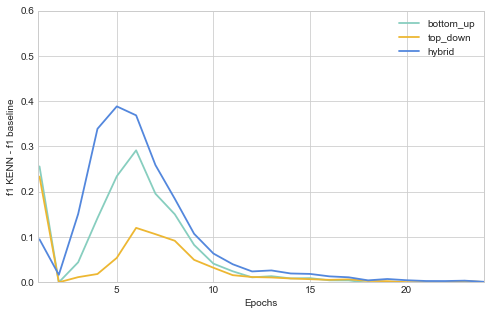
\includegraphics[scale=0.4]{figures/initial_boost.png}
    \caption{Difference between the \textit{macro f1 examples} scores of KENN and baseline models with DistilBERT encoder, evaluated on the dev set of FIGER. The curves are averaged over 3 random seeds. Zoom on the first 25 epochs.}
    \label{fig:initial_boost}
\end{figure}

The trend observed in the \textit{average predictions number} is also detectable by all the other metrics. Figure~\ref{fig:initial_boost} highlights the initial boost of KENN-based models by measuring the difference with respect to the baseline in terms of \textit{macro f1 examples}. The behavior that consolidates as the seeds vary is that Hybrid starts better than Bottom Up, which starts better than Top Down. The baseline model, instead, is the one with the slowest start. The cause of this initial ranking may be that the Hybrid mode can exploit the logical rules of both Bottom Up and Top Down modes. In the second part of the training, instead, the models converge to each other and keep improving together. The results of the final models are reported in Table~\ref{tab:kb_modes_comparison} and are very similar for each KB mode.
% Looking at the graphs in their entirety, there is not a dominant model. However, by looking at the \textit{macro f1 classes} graph we can observe that the baseline model is the only one which never takes the lead.
\begin{figure}
     \centering
     \begin{subfigure}{0.8\textwidth}
         \centering
         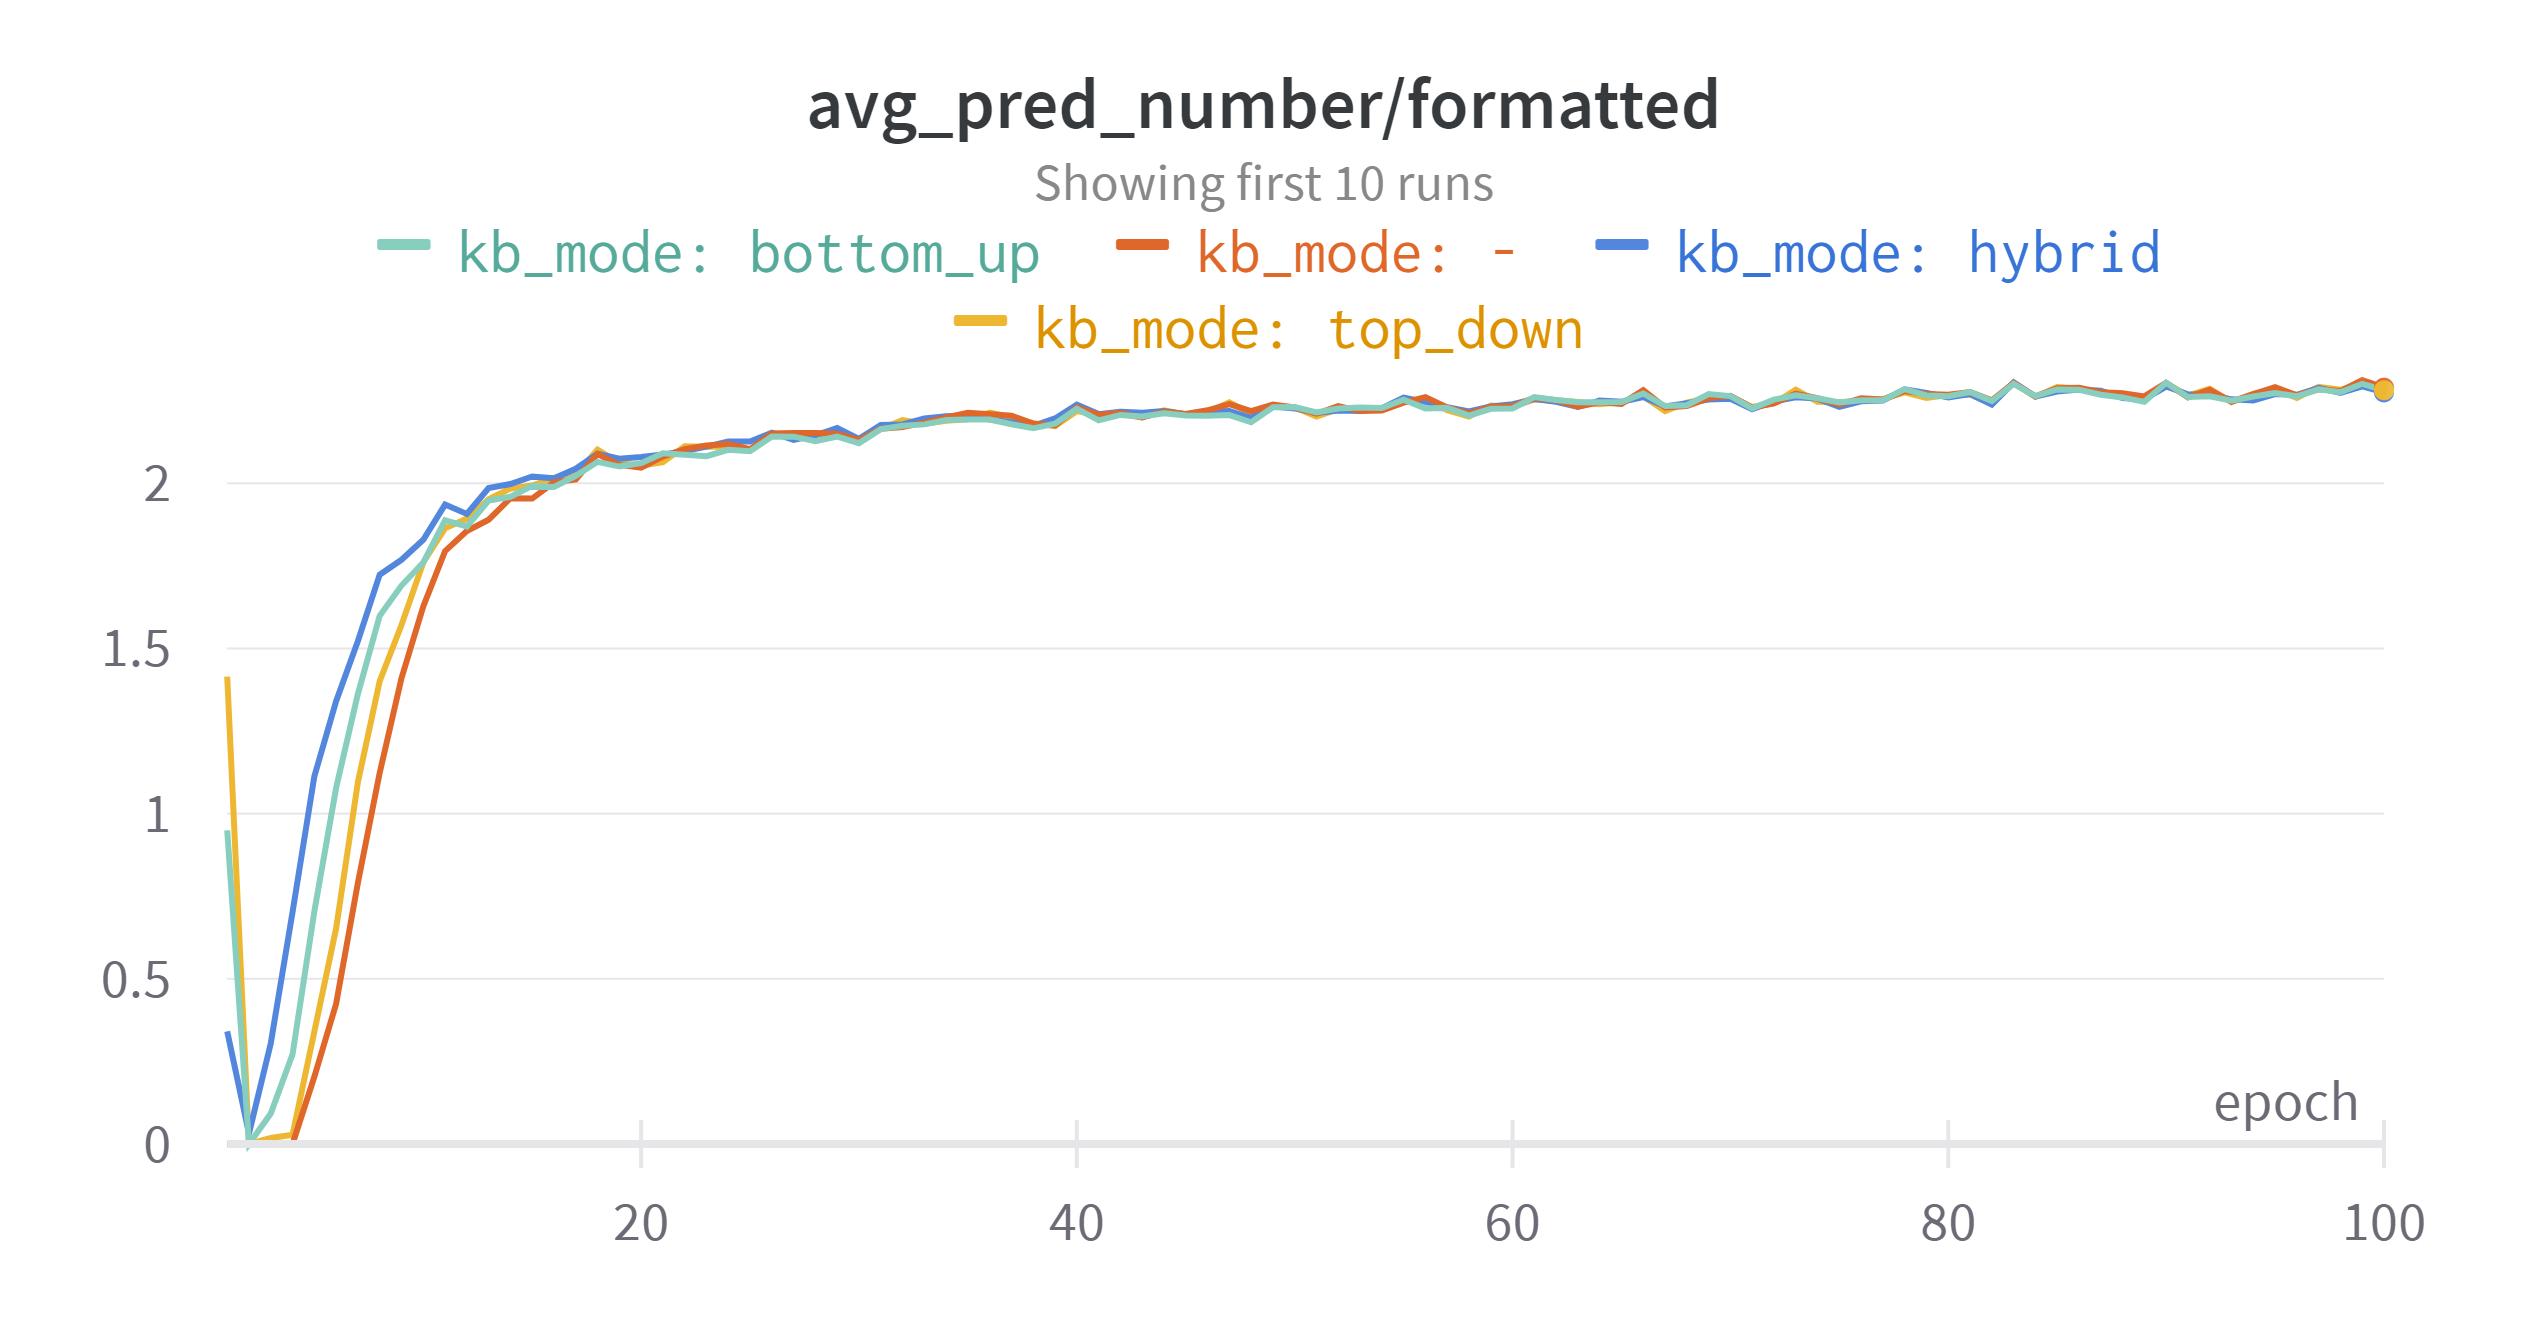
\includegraphics[width=\textwidth]{figures/wandb_modes_avg_pred.png}
         \caption{Average predictions number}
     \end{subfigure}
     \begin{subfigure}{0.8\textwidth}
         \centering
         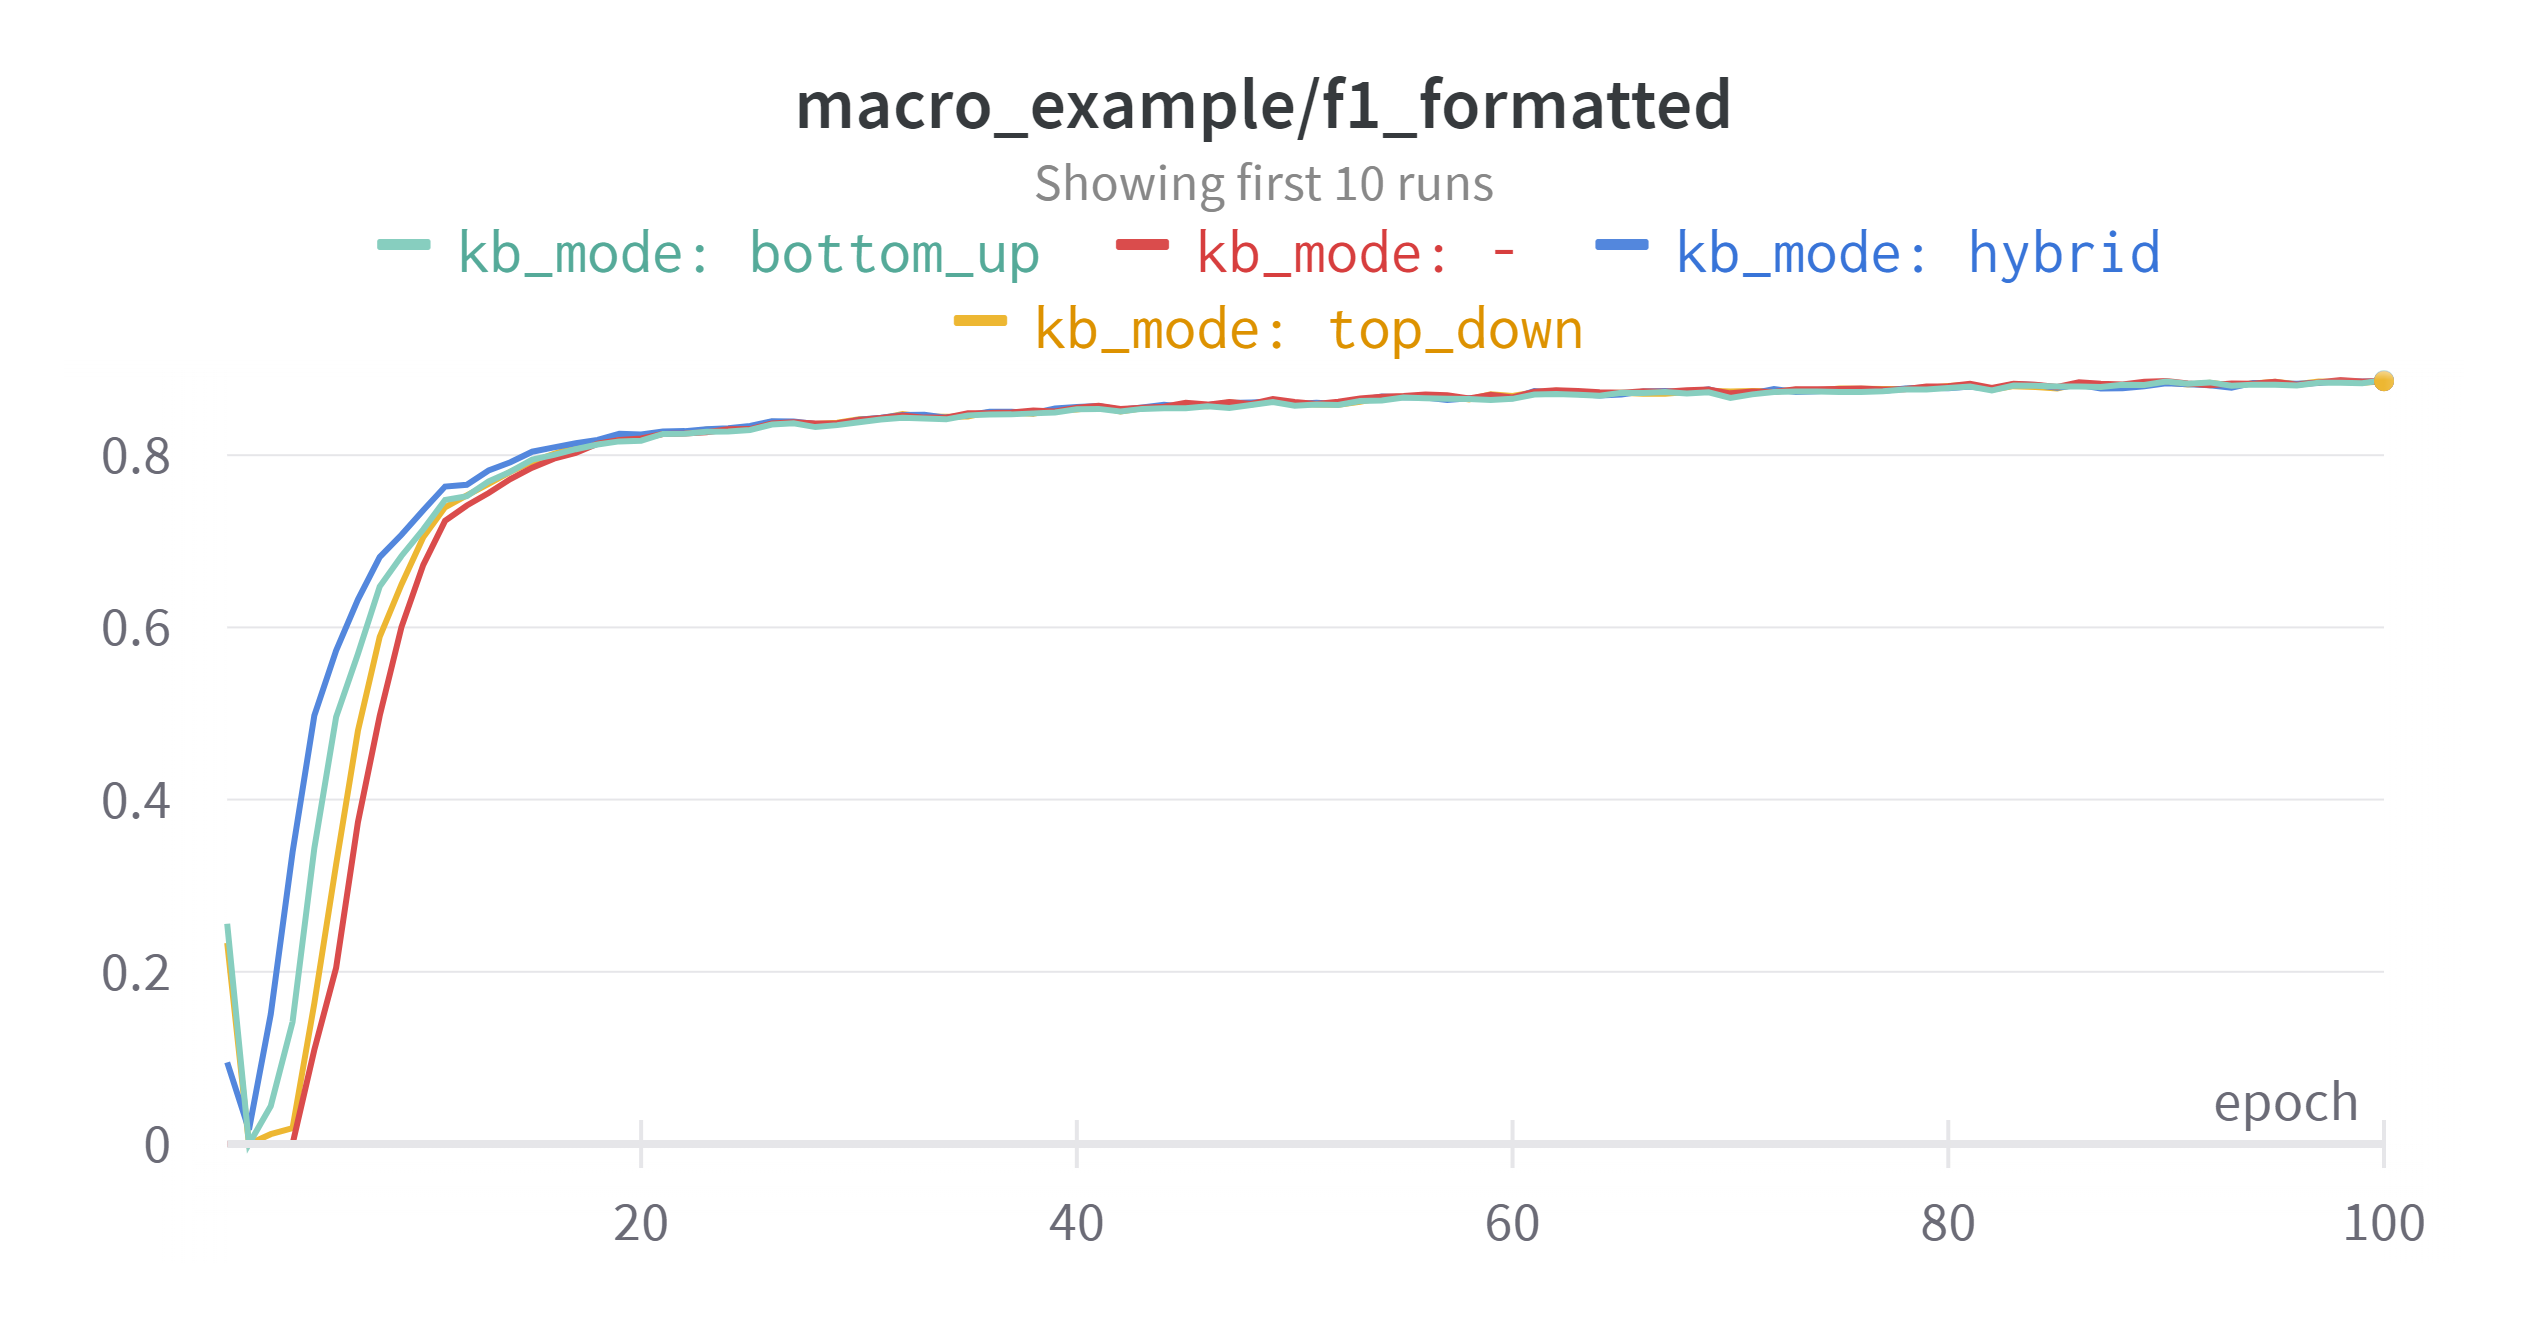
\includegraphics[width=\textwidth]{figures/wandb_modes_macro_ex_f1.png}
         \caption{Macro f1 examples}
     \end{subfigure}
     \begin{subfigure}{0.8\textwidth}
         \centering
         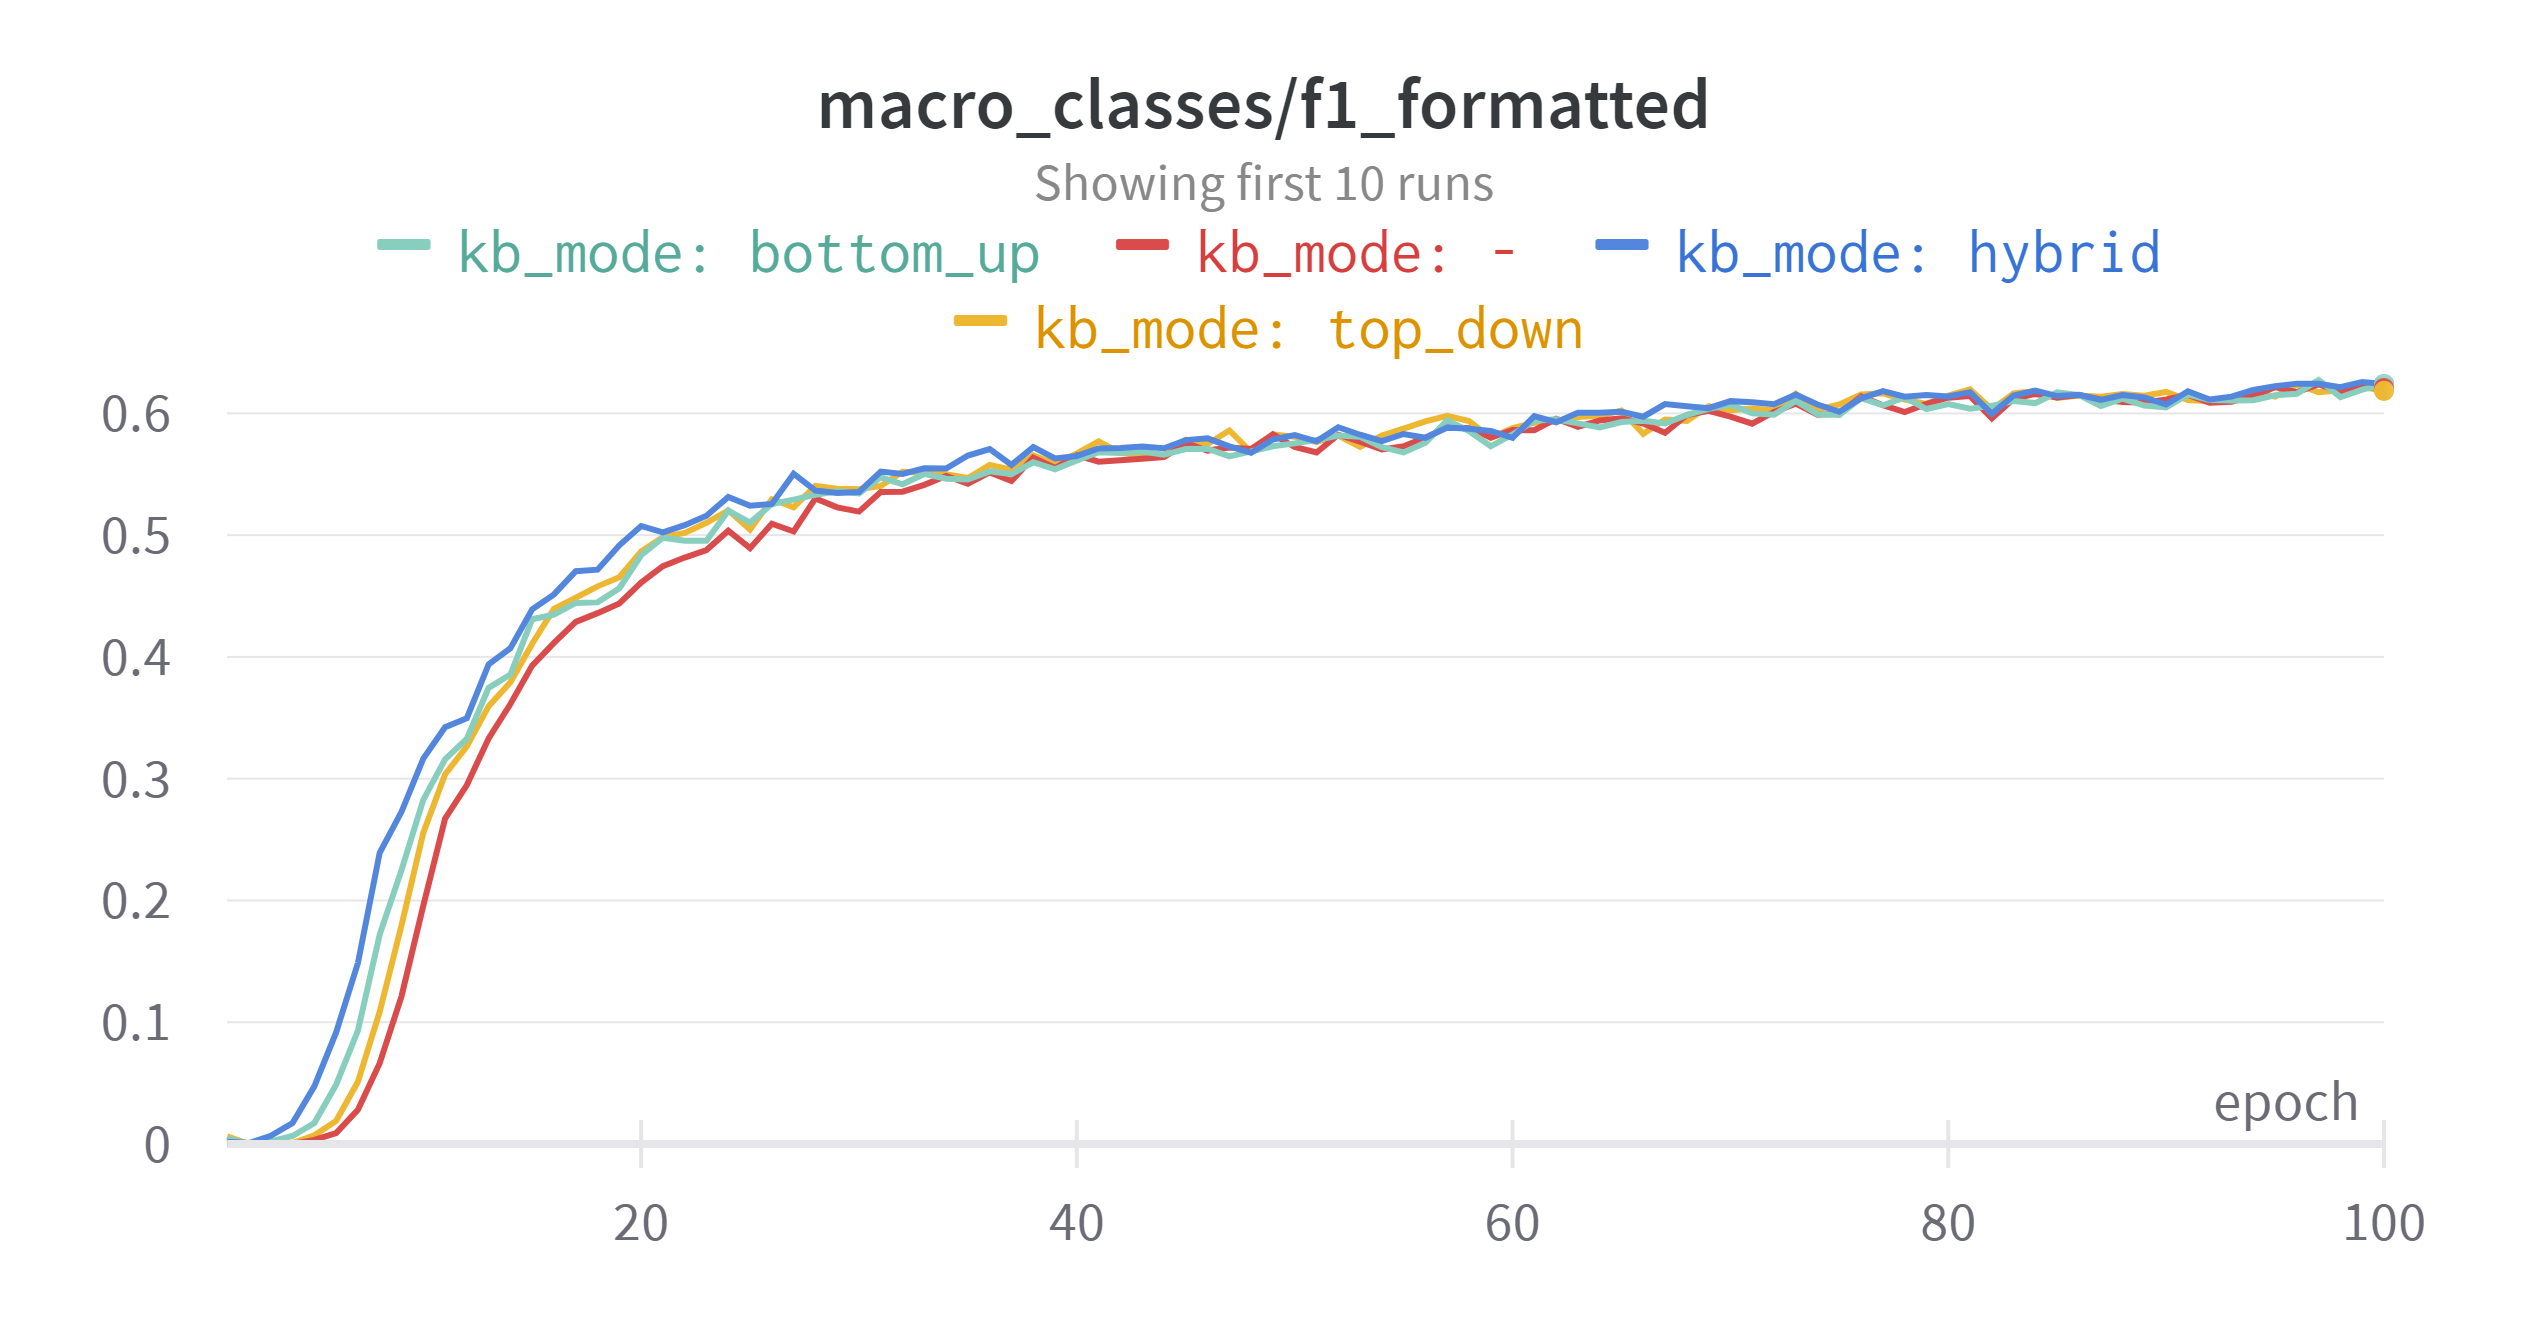
\includegraphics[width=\textwidth]{figures/wandb_modes_macro_class_f1.png}
         \caption{Macro f1 classes}
     \end{subfigure}
        \caption{Comparison between KENN with clause weights fixed to 2.0 and baseline model with DistilBERT encoder, evaluated on the dev set of FIGER. Zoom on the first 20 epochs.}
        \label{fig:wandb_modes_comparison}
\end{figure}

\begin{table}
\centering
\caption{Comparison between KENN with clause weights fixed to 2.0 and baseline model evaluated on the dev set of FIGER. Metrics at epoch 100 averaged over 3 seeds.}
\label{tab:kb_modes_comparison}
\resizebox{\columnwidth}{!}{\begin{tabular}{c|ccc|ccc|}
\cline{2-7}
\textbf{}                            & \multicolumn{3}{c|}{\textbf{Macro examples}}                                                                                                                                                                             & \multicolumn{3}{c|}{\textbf{Macro classes}}                                                                                                                                                                              \\ \hline
\multicolumn{1}{|c|}{\textbf{KB mode}} & \textbf{P}                                                             & \textbf{R}                                                             & \textbf{F1}                                                            & \textbf{P}                                                             & \textbf{R}                                                             & \textbf{F1}                                                            \\ \hline
\multicolumn{1}{|c|}{- (baseline)}       & \begin{tabular}[c]{@{}c@{}}0.8944\\ $\pm$ 0.0009\end{tabular}          & \begin{tabular}[c]{@{}c@{}}0.8779\\ $\pm$ 0.0033\end{tabular}          & \begin{tabular}[c]{@{}c@{}}0.8861\\ $\pm$ 0.0021\end{tabular}          & \begin{tabular}[c]{@{}c@{}}0.6499\\ $\pm$ 0.0152\end{tabular}          & \begin{tabular}[c]{@{}c@{}}0.5943\\ $\pm$ 0.0051\end{tabular}          & \begin{tabular}[c]{@{}c@{}}0.6208\\ $\pm$ 0.0091\end{tabular}          \\ \hline
\multicolumn{1}{|c|}{Bottom Up}      & \begin{tabular}[c]{@{}c@{}}0.8963\\ $\pm$ 0.0.0020\end{tabular}        & \textbf{\begin{tabular}[c]{@{}c@{}}0.8783\\ $\pm$ 0.0047\end{tabular}} & \textbf{\begin{tabular}[c]{@{}c@{}}0.8872\\ $\pm$ 0.0020\end{tabular}} & \begin{tabular}[c]{@{}c@{}}0.6516\\ $\pm$ 0.0165\end{tabular}          & \textbf{\begin{tabular}[c]{@{}c@{}}0.5986\\ $\pm$ 0.0110\end{tabular}} & \begin{tabular}[c]{@{}c@{}}0.6239\\ $\pm$ 0.0115\end{tabular}          \\ \hline
\multicolumn{1}{|c|}{Top Down}       & \begin{tabular}[c]{@{}c@{}}0.8944\\ $\pm$ 0.0008\end{tabular}          & \begin{tabular}[c]{@{}c@{}}0.8777\\ $\pm$ 0.0029\end{tabular}          & \begin{tabular}[c]{@{}c@{}}0.8860\\ $\pm$ 0.0013\end{tabular}          & \begin{tabular}[c]{@{}c@{}}0.6484\\ $\pm$ 0.0088\end{tabular}          & \begin{tabular}[c]{@{}c@{}}0.5913\\ $\pm$ 0.0112\end{tabular}          & \begin{tabular}[c]{@{}c@{}}0.6185\\ $\pm$ 0.0010\end{tabular}          \\ \hline
\multicolumn{1}{|c|}{Hybrid}         & \textbf{\begin{tabular}[c]{@{}c@{}}0.8965\\ $\pm$ 0.0028\end{tabular}} & \begin{tabular}[c]{@{}c@{}}0.8759\\ $\pm$ 0.0025\end{tabular}          & \begin{tabular}[c]{@{}c@{}}0.8861\\ $\pm$ 0.0017\end{tabular}          & \textbf{\begin{tabular}[c]{@{}c@{}}0.6533\\ $\pm$ 0.0185\end{tabular}} & \begin{tabular}[c]{@{}c@{}}0.5974\\ $\pm$ 0.0050\end{tabular}          & \textbf{\begin{tabular}[c]{@{}c@{}}0.6241\\ $\pm$ 0.0112\end{tabular}} \\ \hline
\end{tabular}}
\end{table}

\paragraphn{Quantitative analysis 3 - Metrics per type}
We can observe some interesting behaviors by computing the metrics grouped per types F and S. Focusing on epoch 4 (i.e., the last epoch before the baseline model starts making predictions), it emerges that KENN predicts only types F. This result makes sense since an F type should be easier to predict than an S type, which is more specific. More in detail, Bottom Up and Top Down modes can lead the model to make predictions exclusively on the type \texttt{/location}, reaching an f1 score of 0.595 and 0.441 respectively. The Hybrid model, which achieves an f1 score of 0.747 on \texttt{/location}, can also predict instances of type \texttt{/person} and \texttt{/organization}.

If we now focus on epoch 100, we can observe that Bottom Up performs better than Top Down on types F, with an f1 score of 0.661 and 0.646 respectively. Conversely, if we group the metrics per type S, we can observe that Top Down is better than Bottom Up, with an f1 score of 0.563 and 0.546 respectively. This behavior is consistent with the nature of the different clauses: Bottom Up propagates the information to F, Top Down to S.

\paragraphn{Quantitative analysis - Conclusion}
This analysis points out that the more relevant differences are observable only at the beginning of the training. The initial gap between different clause weights is bridged after 15-20 epochs, as does the difference between the KB modes. The same behavior can be observed when comparing KENN to the baseline model. The suspicion emerging from these considerations is that, at some point of the training, the baseline model becomes as powerful as the KENN-based models. 
%This suspicion can also be extended to the pre-KENN network, which increases its prediction capabilities epoch after epoch, needing less and less KENN's help.
From this premises we can sketch the following hypothesis: the pre-KENN network may adapt its output to obtain some desired predictions after the knowledge enhancement. This hypothesis will be further investigated with the analysis of the preactivations.
\paragraphn{Preactivations analysis 1 - Distributions}
We concluded the quantitative analysis leaving an open question: does the pre-KENN network adapt its predictions to KENN's action? To answer this question, we can start by examining the distribution of the preactivations of every final model. Each distribution will be split into two graphs to simplify the comparison by separating positive and negative predictions using different scales. Figure~\ref{fig:baseline_distrib} shows the distributions of the baseline model that will be used as a reference point. The values of $x$ are the preactivations of each type of each example, while the $y$ represents the frequency of a bin of preactivations.

We will start by comparing the positive predictions. In Figure~\ref{fig:kenn_pos_distrib} we can find the positive distributions of the KENN-based models. The first thing we can observe is that each KB mode produces very different pre-KENN distributions. If we look at the means (Bottom Up: 2.706, Top Down: 3.633, Hybrid: 2.227) and standard deviations (Bottom Up: 1.737, Top Down: 2.190, Hybrid: 1.434), we can also assert that they differ a lot from the baseline positive distribution (mean: 4.246, standard deviation: 2.228). On the contrary, the situation is completely different when looking at the post-KENN preactivations, since the intervention of KENN makes the distributions more similar to each other (means: 4.100$\pm$0.043, standard deviations: 2.058$\pm$0.038) and to the baseline. The same phenomenon can be observed by comparing the negative distribution of the baseline in Figure~\ref{fig:baseline_neg_distrib} to the pre-KENN and post-KENN negative distributions in Figure~\ref{fig:kenn_neg_distrib}.

\begin{figure}[H]
     \centering
     \begin{subfigure}{0.5\textwidth}
         \centering
         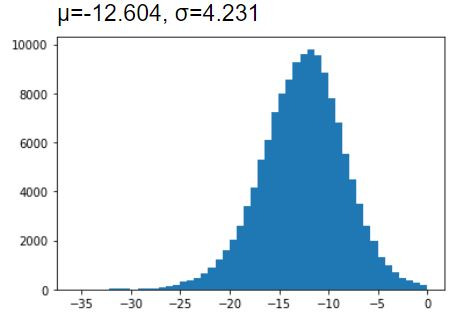
\includegraphics[width=\textwidth]{figures/baseline_neg.JPG}
         \caption{Negative preactivations}
         \label{fig:baseline_neg_distrib}
     \end{subfigure}
     \hfill
     \begin{subfigure}{0.475\textwidth}
         \centering
         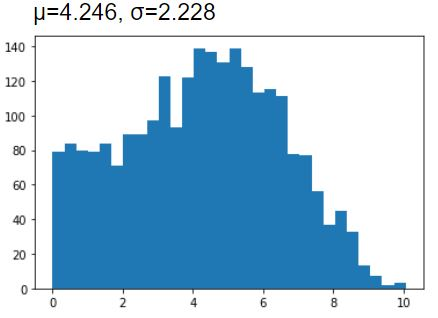
\includegraphics[width=\textwidth]{figures/baseline_pos.JPG}
         \caption{Positive preactivations}
         \label{fig:baseline_pos_distrib}
     \end{subfigure}
        \caption{Distribution of the baseline preactivations computed on the dev set of FIGER}
        \label{fig:baseline_distrib}
\end{figure}


\begin{figure}[H]
    \centering
    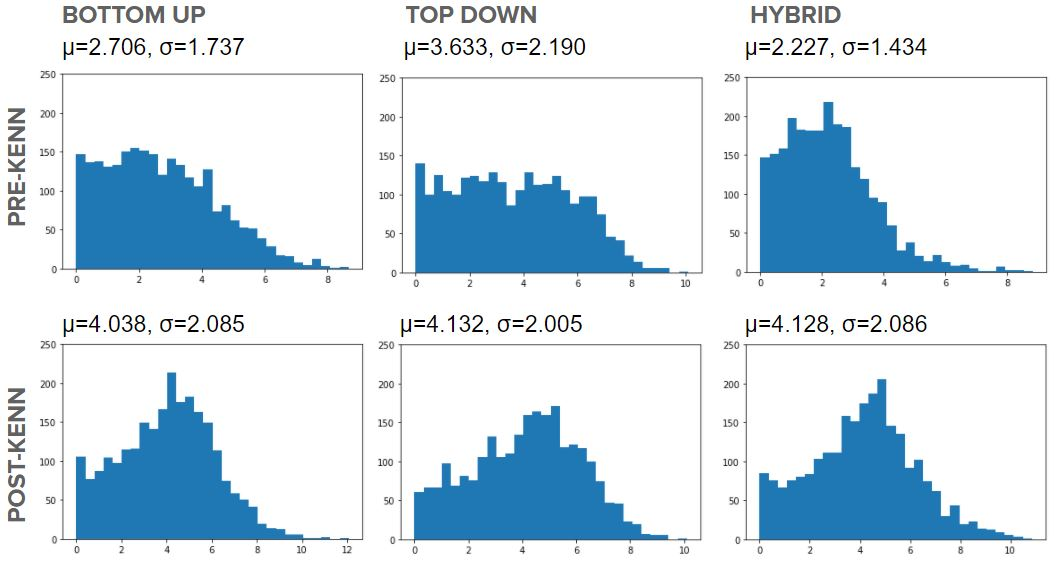
\includegraphics[scale=.53]{figures/kenn_pos_distrib.JPG}
    \caption{Distribution of the pre-KENN and post-KENN positive preactivations for each KB mode. Computed on the dev set of FIGER.}
    \label{fig:kenn_pos_distrib}
\end{figure}

\begin{figure}[H]
    \centering
    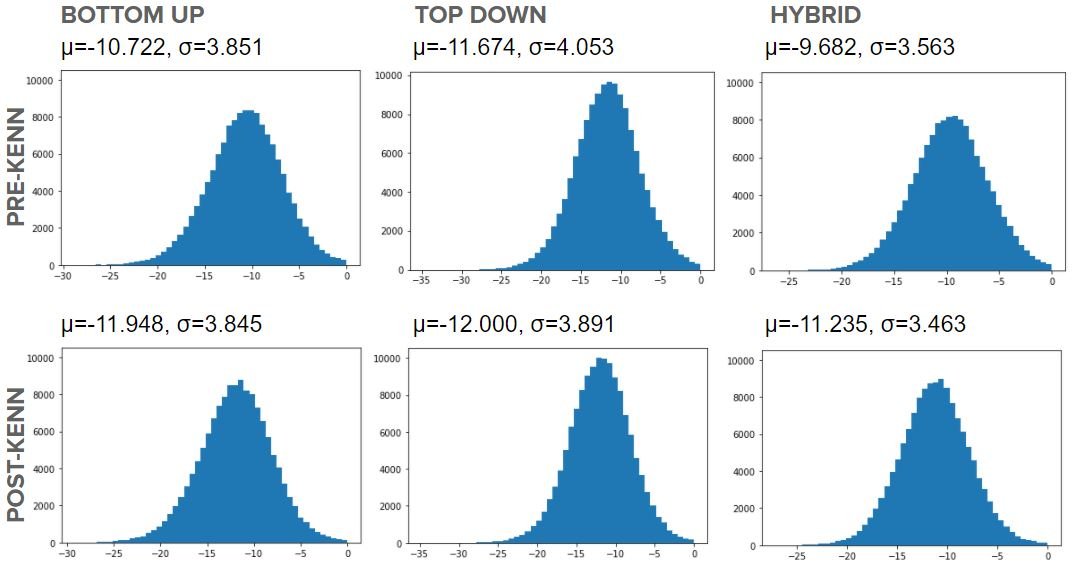
\includegraphics[scale=.53]{figures/kenn_neg_distrib.JPG}
    \caption{Distribution of the pre-KENN and post-KENN negative preactivations for each KB mode. Computed on the dev set of FIGER.}
    \label{fig:kenn_neg_distrib}
\end{figure}

\paragraphn{Preactivations analysis 2 and 3 - FSM and Sankey diagrams}
The analysis of the Finite State Machines and the Sankey diagrams can help to understand how the pre-KENN and post-KENN preactivations are modified depending on types F and S involved in the same clause, thus providing other insights into the suspicion of adaptation emerged in the previous study.

Starting from the Bottom Up mode, we can find the FSM and the Sankey diagram in Figure~\ref{fig:transitions_bottom_up}. We remind that a Bottom Up clause will always produce a positive delta on F and a negative delta on S. Indeed, F1S0 is a sink vertex of the Bottom Up FSM because F can never be decreased and S can never be increased in a Bottom Up setup. By analyzing the information of the transitions, we can observe that:
\begin{enumerate}
    \item The percentages of wrong transitions represent a minority.
    \item The probability of remaining in the forbidden state (i.e., F0S1) is 0.03. This is reasonable because the forbidden state represents also a clause violation (i.e., 1$\to$0) for this KB mode, so KENN will always try to modify the predictions to reach another post-KENN state. In these cases, the percentages of correctness show that the outgoing transitions from F0S1 never lead to worse predictions, but this is trivial since it is a wrong state by definition.
    \item The statistics about the transition F0S1$\to$F1S0 are quite counterintuitive since F and S are reversed correctly in 43.1\% of cases. The fact that the pre-KENN network predicts F as negative and S as positive when the target is the opposite is curious. It is plausible that the pre-KENN network learned that a type F usually receives one or more positive boosts, so it produces an initial negative prediction being aware that KENN will correct the final value. 
    \item The transition F0S0$\to$F1S0 could seem weird too. It has a probability of 0.01 and a percentage of correctness of 84.3\%. Some of these transitions are due to the fact that in the Bottom Up mode a type F is involved in multiple clauses, so the positive boost could derive from one or more siblings of S. However, after an investigation, it emerged that there are several examples of transitions F0S$_{1,...,n}$0$\to$F1S$_{1,...,n}$0 where F becomes positive thanks to the aggregated boost of its negative children. In particular, on a total of 500 F0S0$\to$F1S0 transitions, in 78 of them the effect of a single S was sufficient to enhance F. Even this behavior could be explained by the fact that the pre-KENN network learned that F is used to receive positive boosts.
\end{enumerate}


\begin{figure}
     \centering
     \begin{subfigure}{0.7\textwidth}
         \centering
         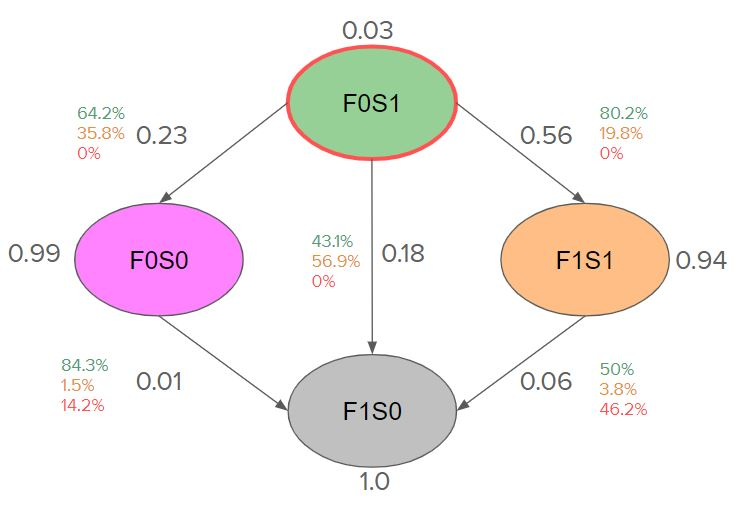
\includegraphics[width=\textwidth]{figures/fsm_bottom_up.JPG}
         \caption{FSM}
         \label{fig:fsm_bottom_up}
         \vspace{15px}
     \end{subfigure}
     \vfill
     \begin{subfigure}{0.6\textwidth}
         \centering
         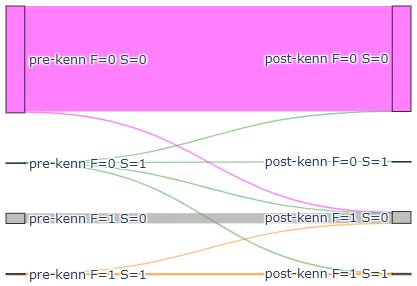
\includegraphics[width=\textwidth]{figures/sankey_bottom_up.JPG}
         \caption{Sankey diagram}
         \label{fig:sankey_bottom_up}
     \end{subfigure}
        \caption{FSM and Sankey diagram of the Bottom Up mode on the dev set of FIGER.}
        \label{fig:transitions_bottom_up}
\end{figure}

The FSM and the Sankey diagram of the Top Down mode are shown in Figure~\ref{fig:transitions_top_down}. The first thing we can notice is that the transitions of the FSM have opposite directions with respect to Bottom Up, so the sink vertex becomes F0S1. Looking at the statistics of the transitions, we can observe that:
\begin{enumerate}
    \item The percentages of wrong transitions represent a minority.
    \item The incoming transitions of the forbidden state have null probabilities when starting from F0S0 or F1S1, and near-zero probability when the pre-KENN state is F1S0. This is a very interesting fact, since it means that the pre-KENN network produces predictions such that KENN cannot generate a boost that leads to the forbidden state.
    \item Even if in this KB mode the pre-KENN state F1S0 may represent a clause violation (i.e., 1$\to 0 \vee ... \vee 0$) that KENN will try to correct, we can still find some examples of self-loop transition. Note that the high probability of 0.867 is due to the fact that in a Top Down clause the consequent is a disjunction of siblings. However, if we exclude from the count the cases in which a sibling of S is positive, we still have a high probability of 0.512 of self-loop. This means that the pre-KENN network learned to generate preactivations that prevent the effect of KENN when the desired output is F1S0.
    \item If we look at the Sankey diagram in Figure~\ref{fig:sankey_top_down}, we can see that the pre-KENN state F0S1 (i.e., the sink node) is missing. In this case too, the reason can be found in the fact that the pre-KENN network is aware that KENN will not be able to change the final predictions.
\end{enumerate}

\begin{figure}
     \centering
     \begin{subfigure}{0.7\textwidth}
         \centering
         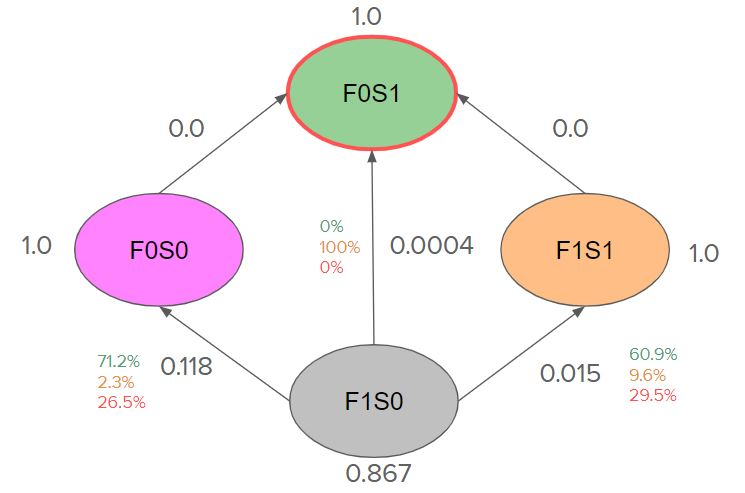
\includegraphics[width=\textwidth]{figures/fsm_top_down.JPG}
         \caption{FSM}
         \label{fig:fsm_top_down}
         \vspace{15px}
     \end{subfigure}
     \vfill
     \begin{subfigure}{0.6\textwidth}
         \centering
         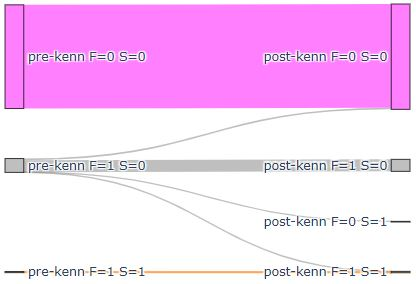
\includegraphics[width=\textwidth]{figures/sankey_top_down.JPG}
         \caption{Sankey diagram}
         \label{fig:sankey_top_down}
     \end{subfigure}
        \caption{FSM and Sankey diagram of the Top Down mode on the dev set of FIGER.}
        \label{fig:transitions_top_down}
\end{figure}

Finally, we can find the transitions of the Hybrid mode in Figure~\ref{fig:transitions_hybrid}. The FSM transitions are bidirectional because they are inherited from Top Down and Bottom Up. The consequence is that there are no sink nodes and all the transitions become potentially available. The considerations we can make by observing the figures are that:
\begin{enumerate}
    \item The percentages of wrong transitions represent a minority.
    \item Similarly to what happens in the Top Down, the probability to make a transition into the forbidden state is null.
    \item The probability of remaining in the forbidden state is very low like in the Bottom Up.
    \item The Sankey diagram is denser than those of Bottom Up and Top Down, since it is constituted by the mix of their transitions.
\end{enumerate}

\begin{figure}
     \centering
     \begin{subfigure}{0.7\textwidth}
         \centering
         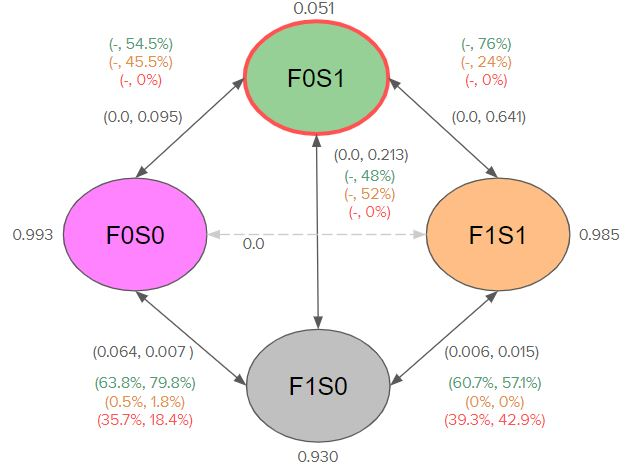
\includegraphics[width=\textwidth]{figures/fsm_hybrid.JPG}
         \caption{FSM - perecentages and probabilities are reported as \textit{(x, y)}, where \textit{x~=~value~of~down-to-up~transition} and \textit{y~=~value~of~up-to-down~transition}  }
         \label{fig:fsm_hybrid}
         \vspace{15px}
     \end{subfigure}
     \vfill
     \begin{subfigure}{0.6\textwidth}
         \centering
         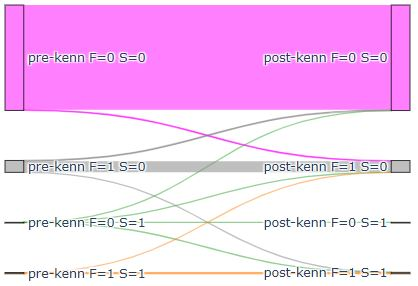
\includegraphics[width=\textwidth]{figures/sankey_hybrid.JPG}
         \caption{Sankey diagram}
         \label{fig:sankey_hybrid}
     \end{subfigure}
        \caption{FSM and Sankey diagram of the Hybrid mode on the dev set of FIGER.}
        \label{fig:transitions_hybrid}
\end{figure}

A final consideration can be done by comparing the three Sankey diagrams: even if their starting states are quite different, their final states become very similar. This fact is analogous to what we observed when comparing the pre-KENN and post-KENN preactivations.

\paragraphn{Preactivation analysis - Conclusion}
This study brought to light several aspects that confirmed the suspicion of adaptation. In the first analysis we saw that while the pre-KENN distributions had relevant differences, the post-KENN distributions became more similar to each other and to the baseline. We then detected other evident signals of adaptation by analyzing the transitions of the FSMs and the Sankey diagrams. Considering the Bottom Up mode, the most representative examples can be found in the transitions F0S1$\to$F1S0 and F0S0$\to$F1S0, where the pre-KENN network seems to be aware of the boost that will be produced on F by KENN. Even more interesting is the situation of the Top Down. Here, the strongest adaptation signals are given by the absence of F0S1 (i.e., sink node) as pre-KENN state in the Sankey diagram and by the high probability of not correcting a violated clause (i.e., self-loop on F1S0).
\subsection{KENN with different encoders: DistilBERT vs BERT} \label{distilbert_vs_bert}
Choosing the right language model is always important to determine the performance of the final model, especially if the goal is to compete with state-of-the-art solutions. This experiment aims to compare the behavior of KENN when dealing with networks based on encoders with different capabilities, which in our case are DistilBERT and BERT.

\subsubsection{Setup}
The models used for this experiment are trained using the \textit{Setup B}. The experimental parameters chosen are the following:
\begin{itemize}
    \item \textbf{KB modes:} Bottom Up, Top Down and Hybrid
    \item \textbf{initial clause weight:} 2.0
    \item \textbf{fixed clause weights}
    \item \textbf{encoder:} DistilBERT and BERT, with adapters
    \item \textbf{loss function:} Binary Cross-Entropy, with the weights of positive examples set to 1
\end{itemize}
This results in a total of 6 configurations. The choice of using fixed clause weights set to 2.0 comes from the previous experiments since it has been observed that higher weights led to higher boosts in the early stage of the training. The experiments are evaluated in terms of \textit{macro f1 examples} by averaging the performance obtained from 3 random seeds per model.

\subsubsection{Results on FIGER}
We can start by comparing the performance obtained by the baseline model with different encoders. Looking at the graph in Figure~\ref{fig:wandb_figer_baseline_distilbert_vs_bert}, we can observe a significant gap between the models. The difference, which is larger at the beginning, persists for the duration of the training and shows the major capabilities of BERT. The final models reach a score of 0.9155 and 0.8911 for BERT and DistilBERT, respectively.
\begin{figure}[bth]
    \centering
    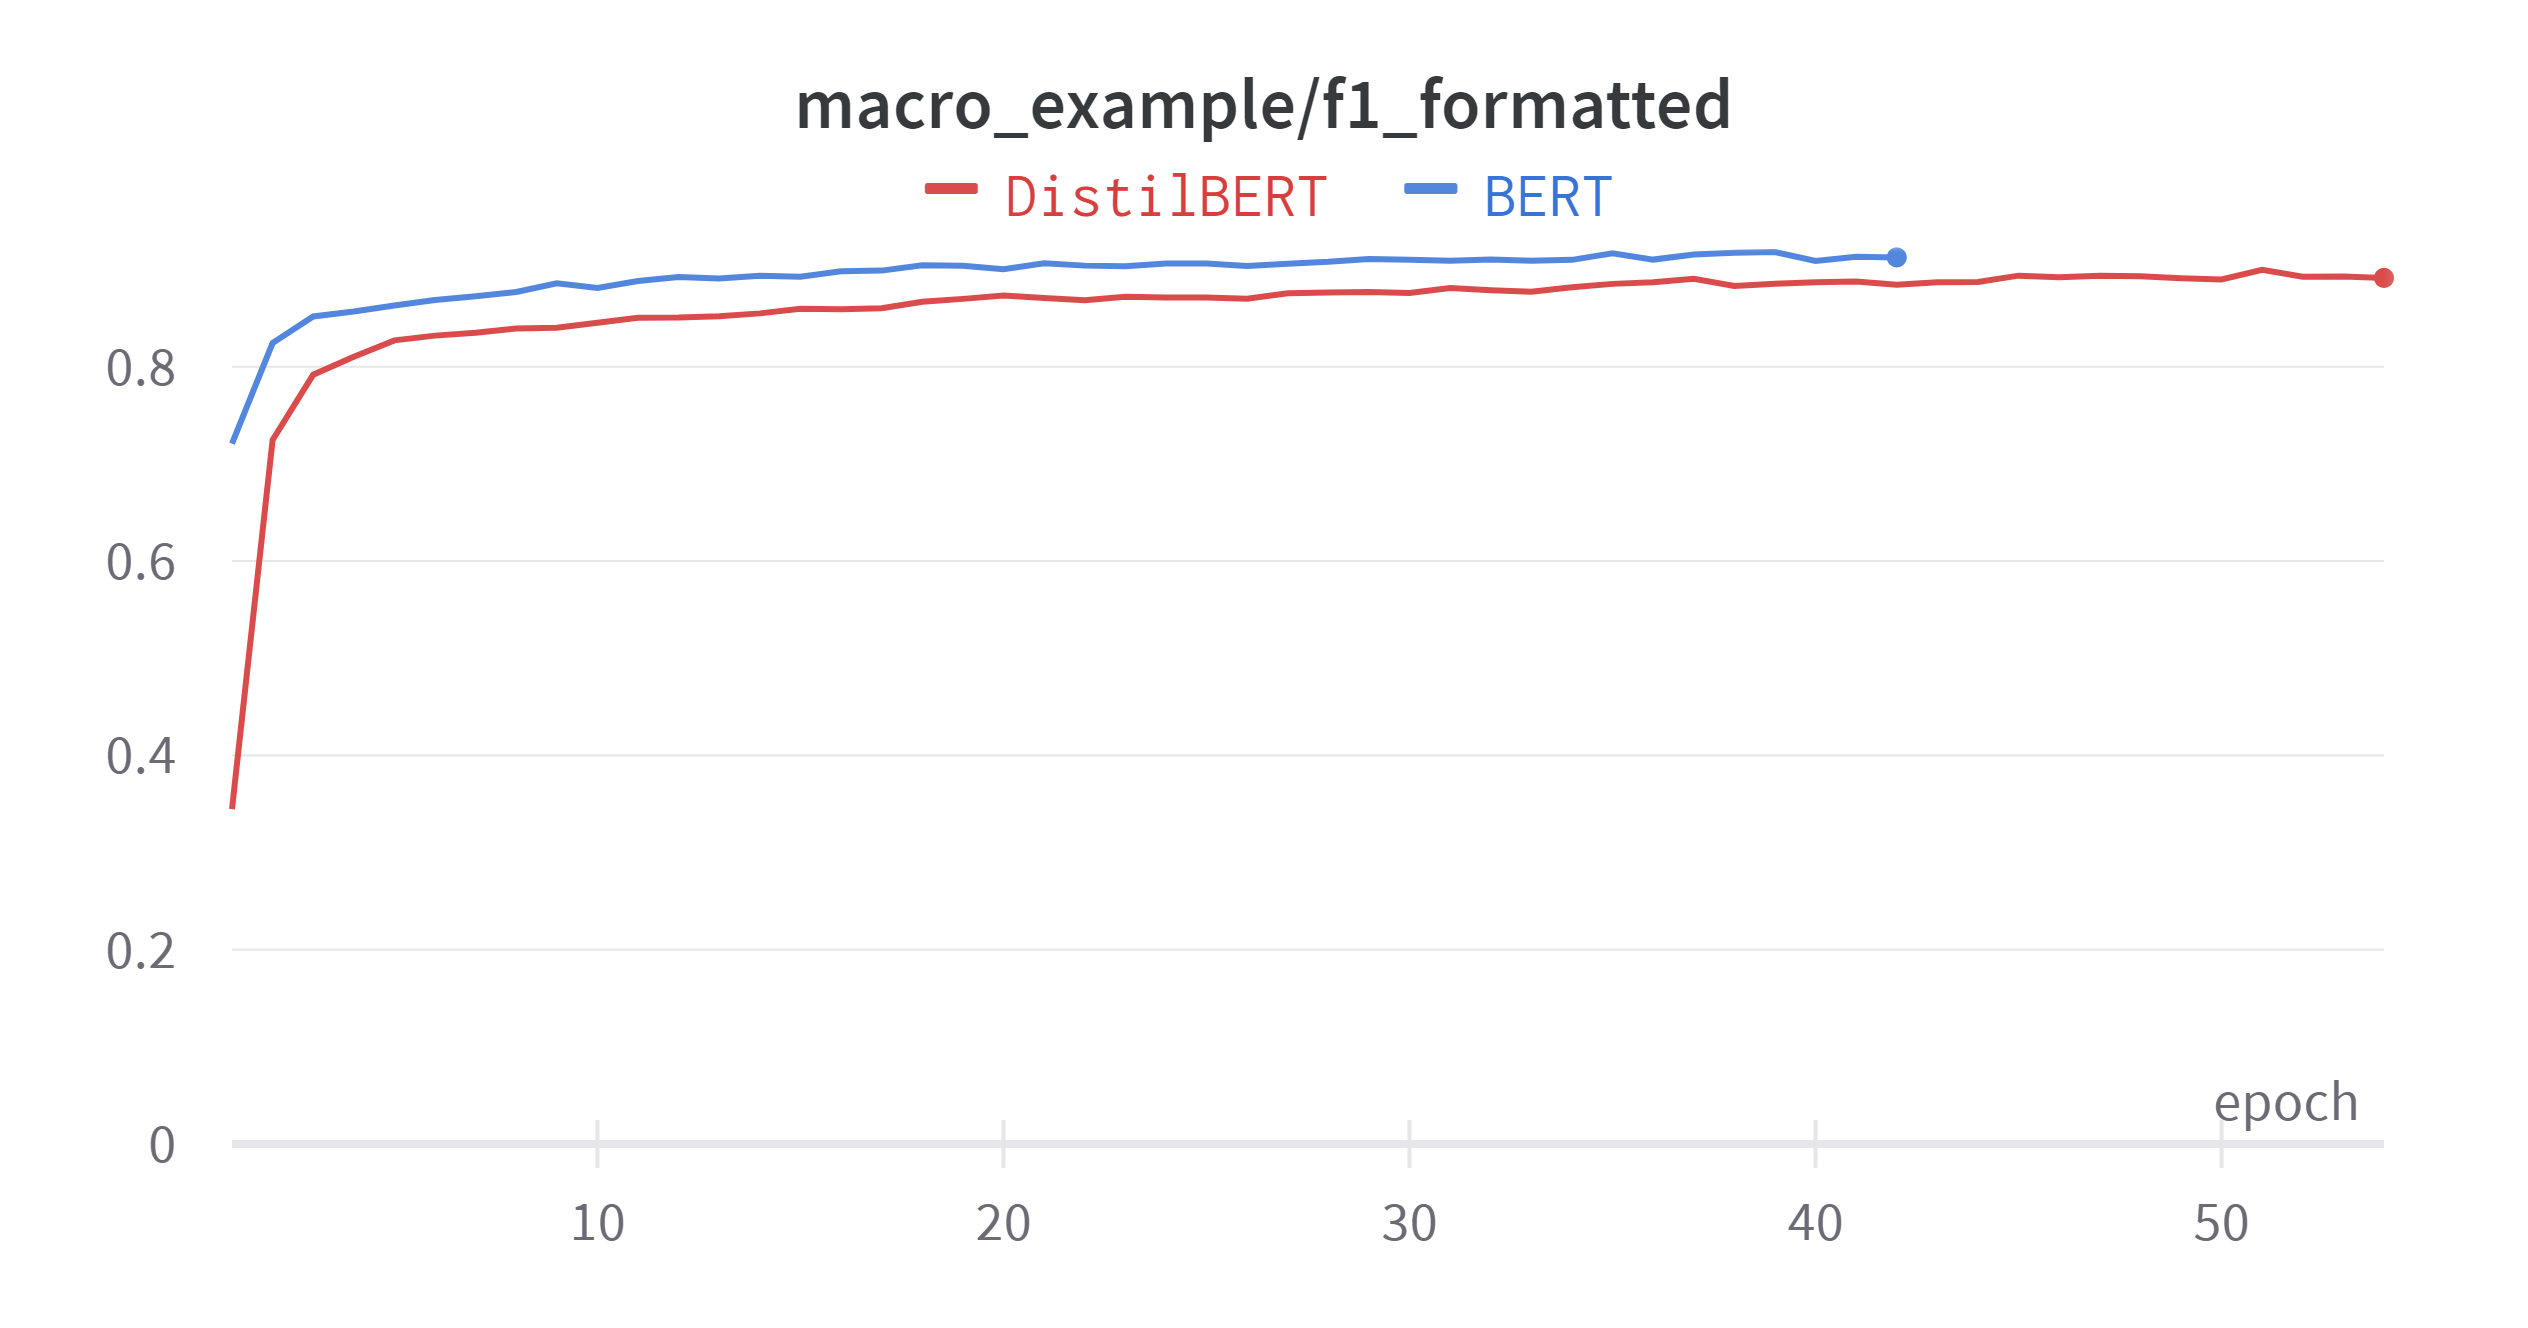
\includegraphics[width=.8\linewidth]{figures/wandb_figer_baseline_distilbert_vs_bert.png}
    \caption{Baseline DistilBERT vs Baseline BERT in terms of \textit{macro f1 examples} on the dev set of FIGER}
    \label{fig:wandb_figer_baseline_distilbert_vs_bert}
\end{figure}

Now that the superiority of BERT has been confirmed, we can proceed with the comparison between the baseline and KENN-based models. In Figures~\ref{fig:wandb_figer_kenn_distilbert} and \ref{fig:wandb_figer_kenn_bert} are presented the performance obtained with DistilBERT and BERT, respectively. As we can see, the behavior of KENN is completely different depending on the encoder. Starting from DistilBERT, the initial boost given by KENN is clearly visible, especially when comparing the baseline to the Hybrid model. However, as already discussed in the quantitative analysis, this boost vanishes in the rest of the training when the models converge. When using BERT, instead, the baseline model is the one that has the best start. While Top Down has a similar training trend even at the beginning, Bottom Up and Hybrid are always inferior.

\begin{figure}[bth]
    \centering
    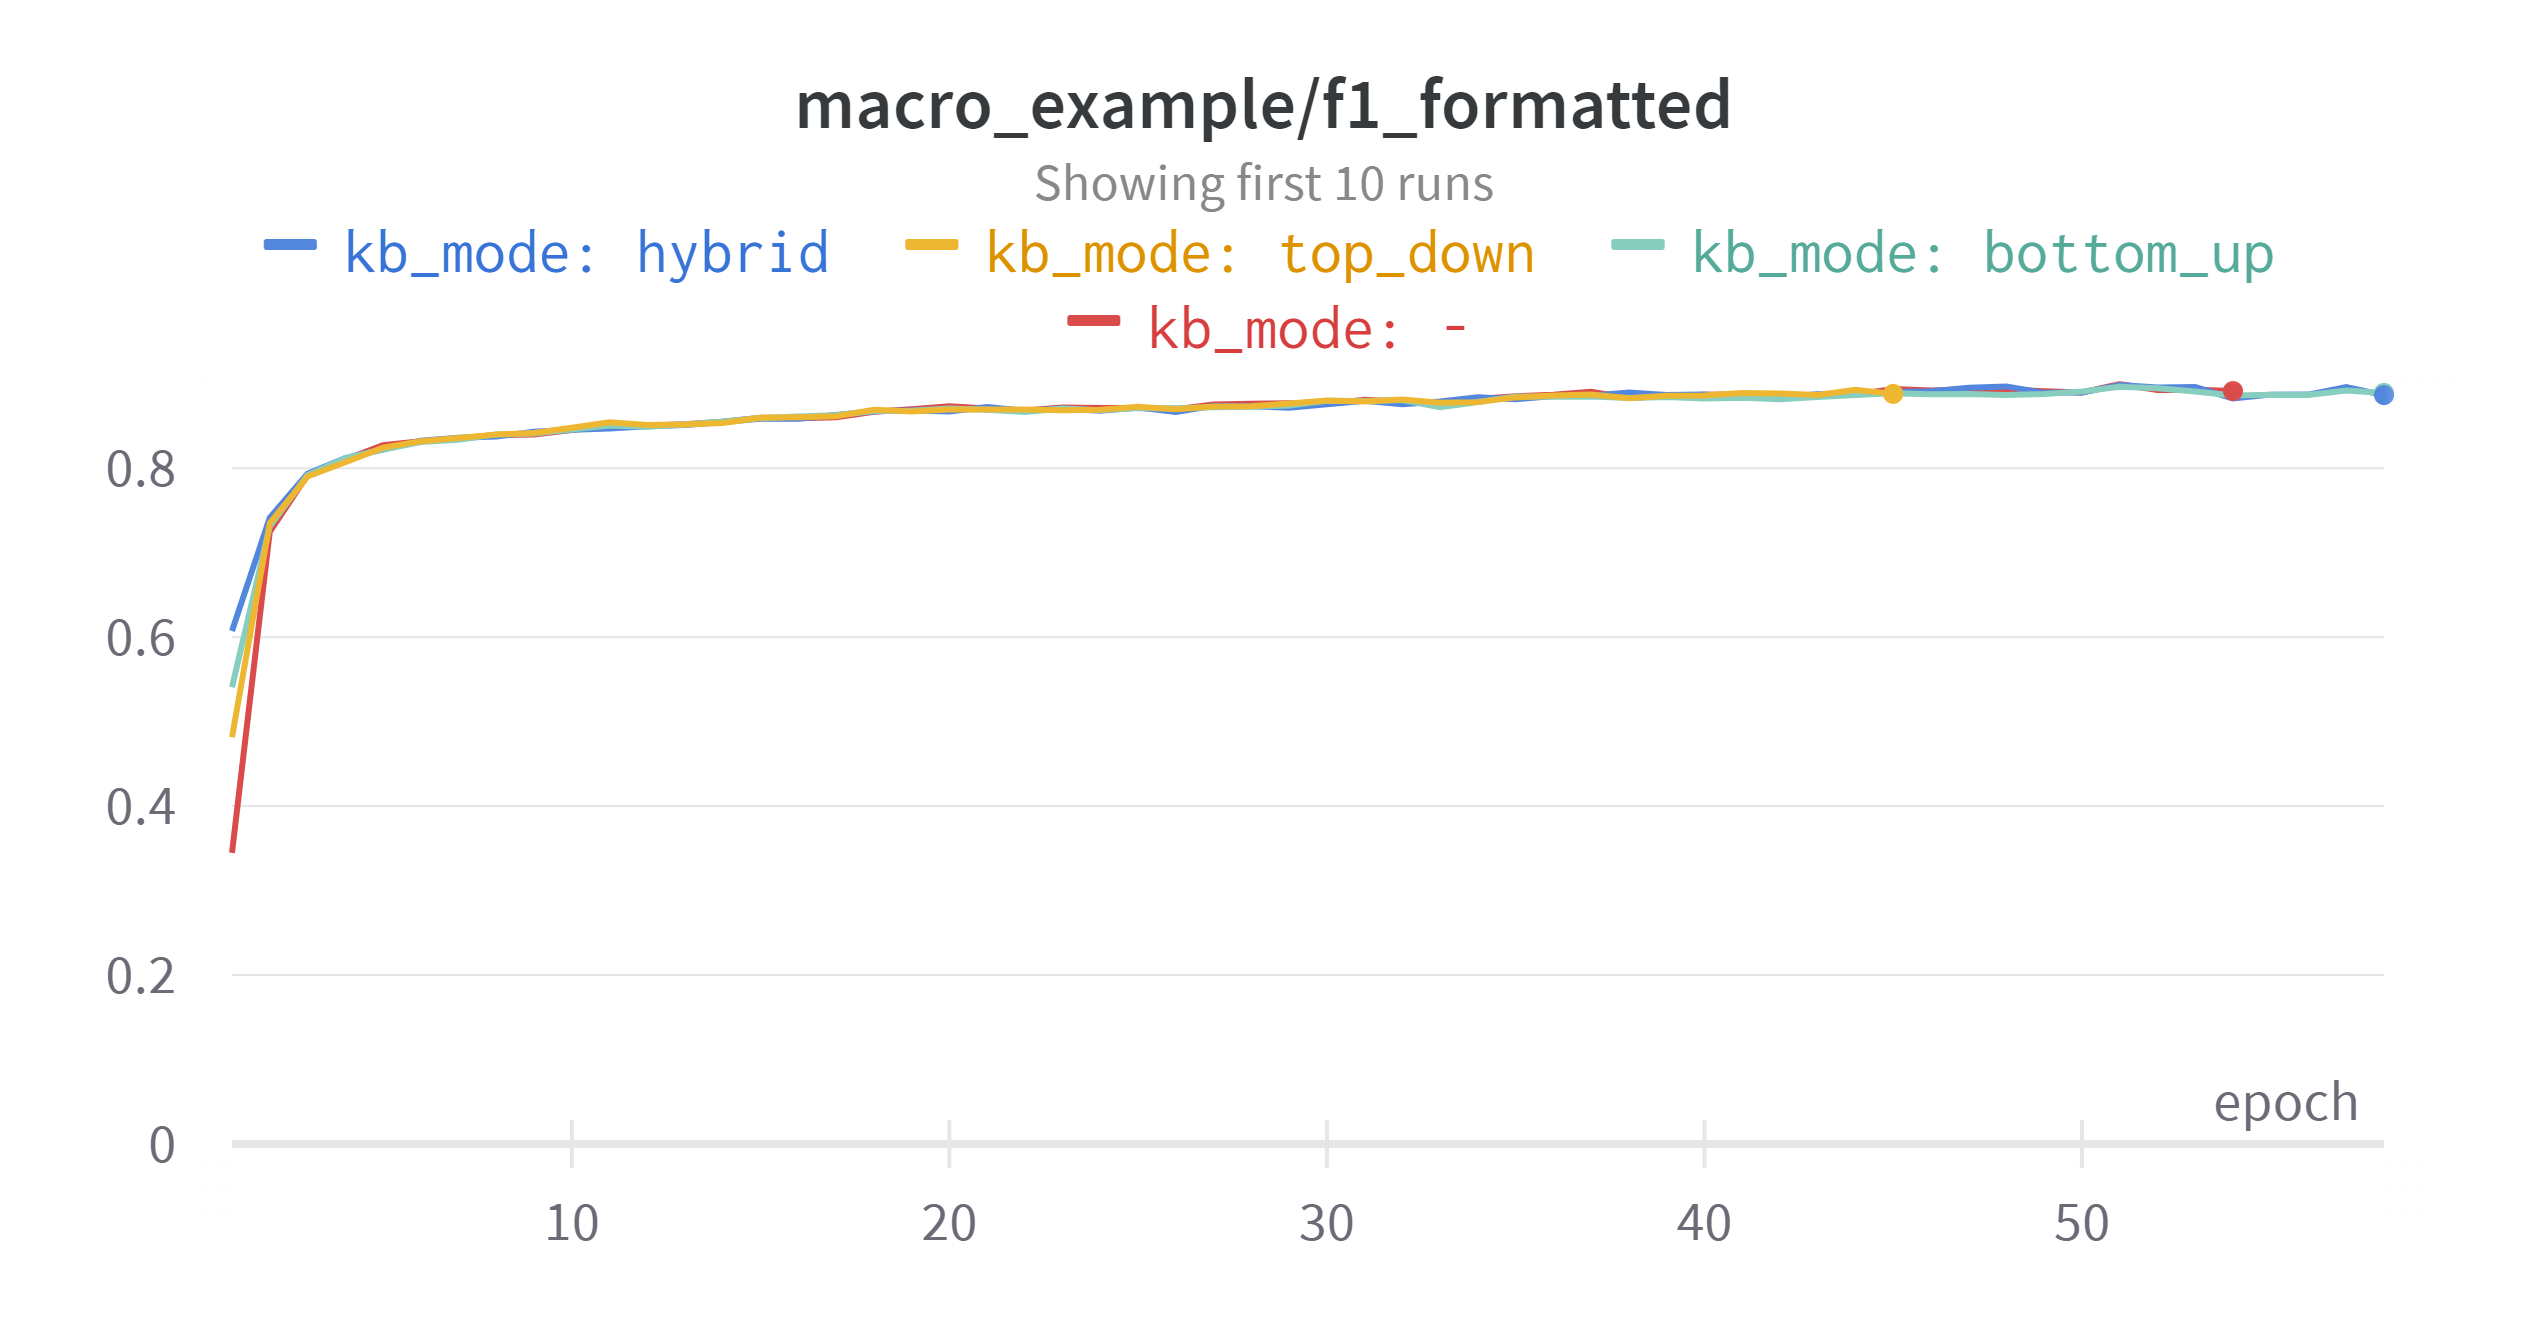
\includegraphics[width=.8\linewidth]{figures/wandb_figer_kenn_distilbert.png}
    \caption{Baseline DistilBERT vs KENN DistilBERT in terms of \textit{macro f1 examples} on the dev set of FIGER.}
    \label{fig:wandb_figer_kenn_distilbert}
\end{figure}

\begin{figure}[bth]
    \centering
    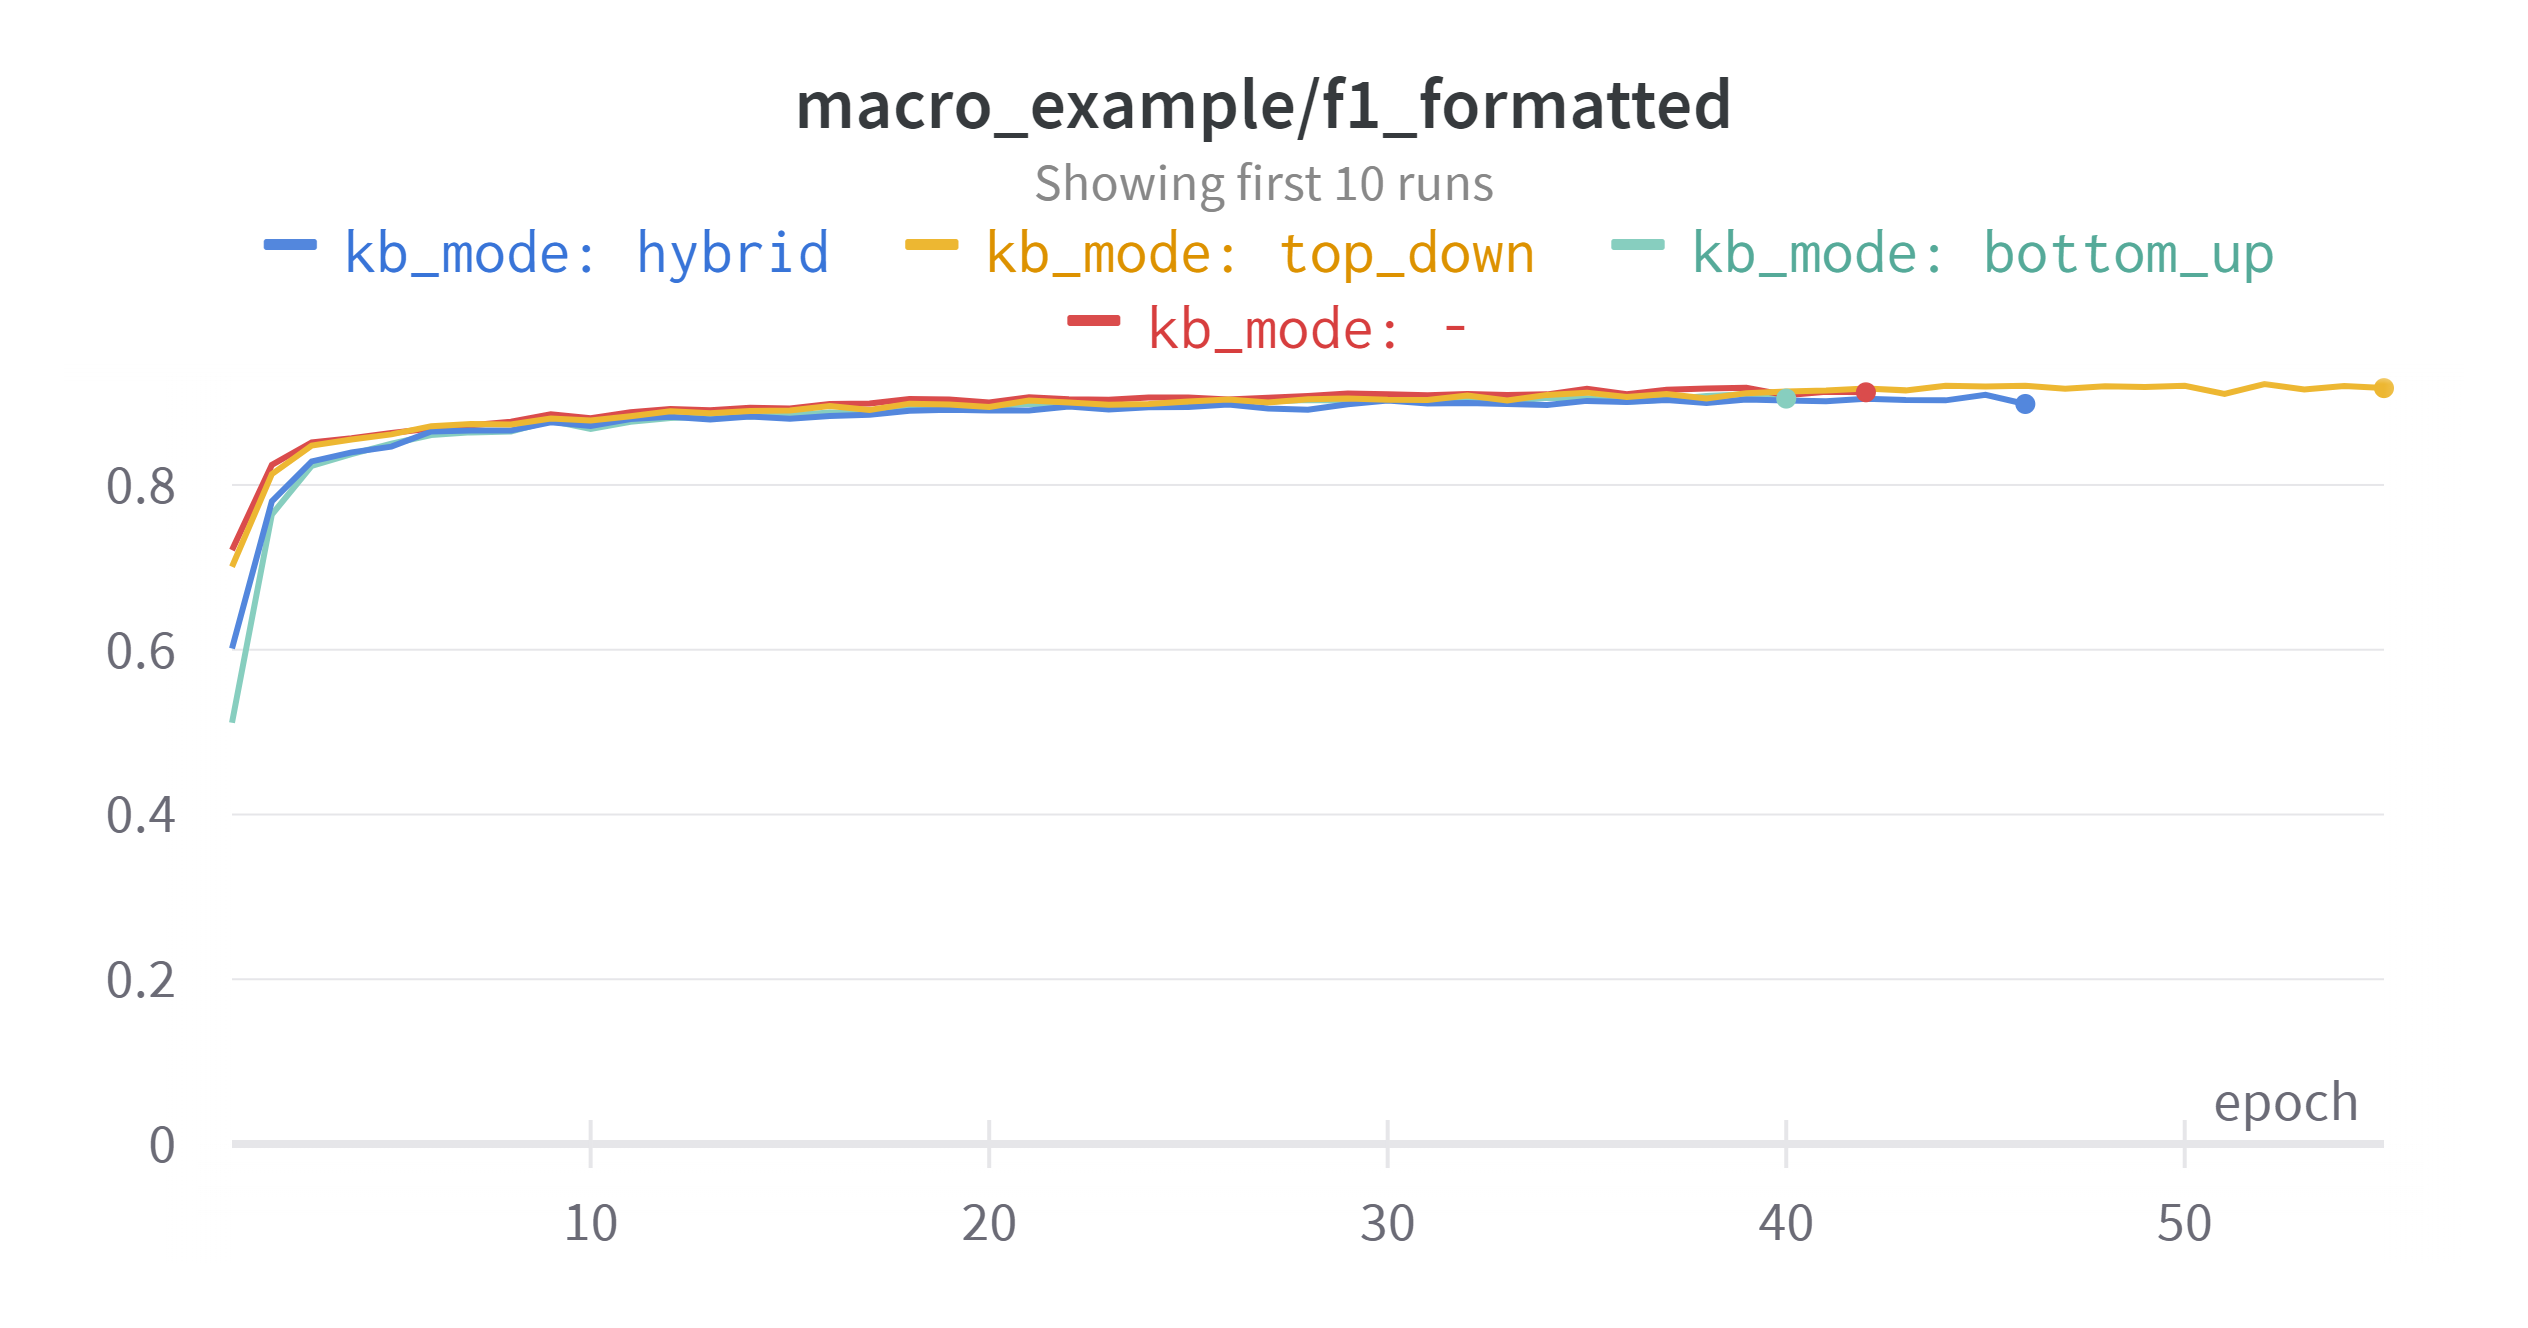
\includegraphics[width=.8\linewidth]{figures/wandb_figer_kenn_bert.png}
    \caption{Baseline BERT vs KENN BERT in terms of \textit{macro f1 examples} on the dev set of FIGER.}
    \label{fig:wandb_figer_kenn_bert}
\end{figure}




\subsubsection{Results on BBN}
Figure~\ref{fig:wandb_bbn_baseline_distilbert_vs_bert} compares DistilBERT and BERT when using the baseline model. Even this dataset confirmed the superiority of BERT, which reached the score of 0.9047, while DistilBERT's score is 0.8845.

\begin{figure}[bth]
    \centering
    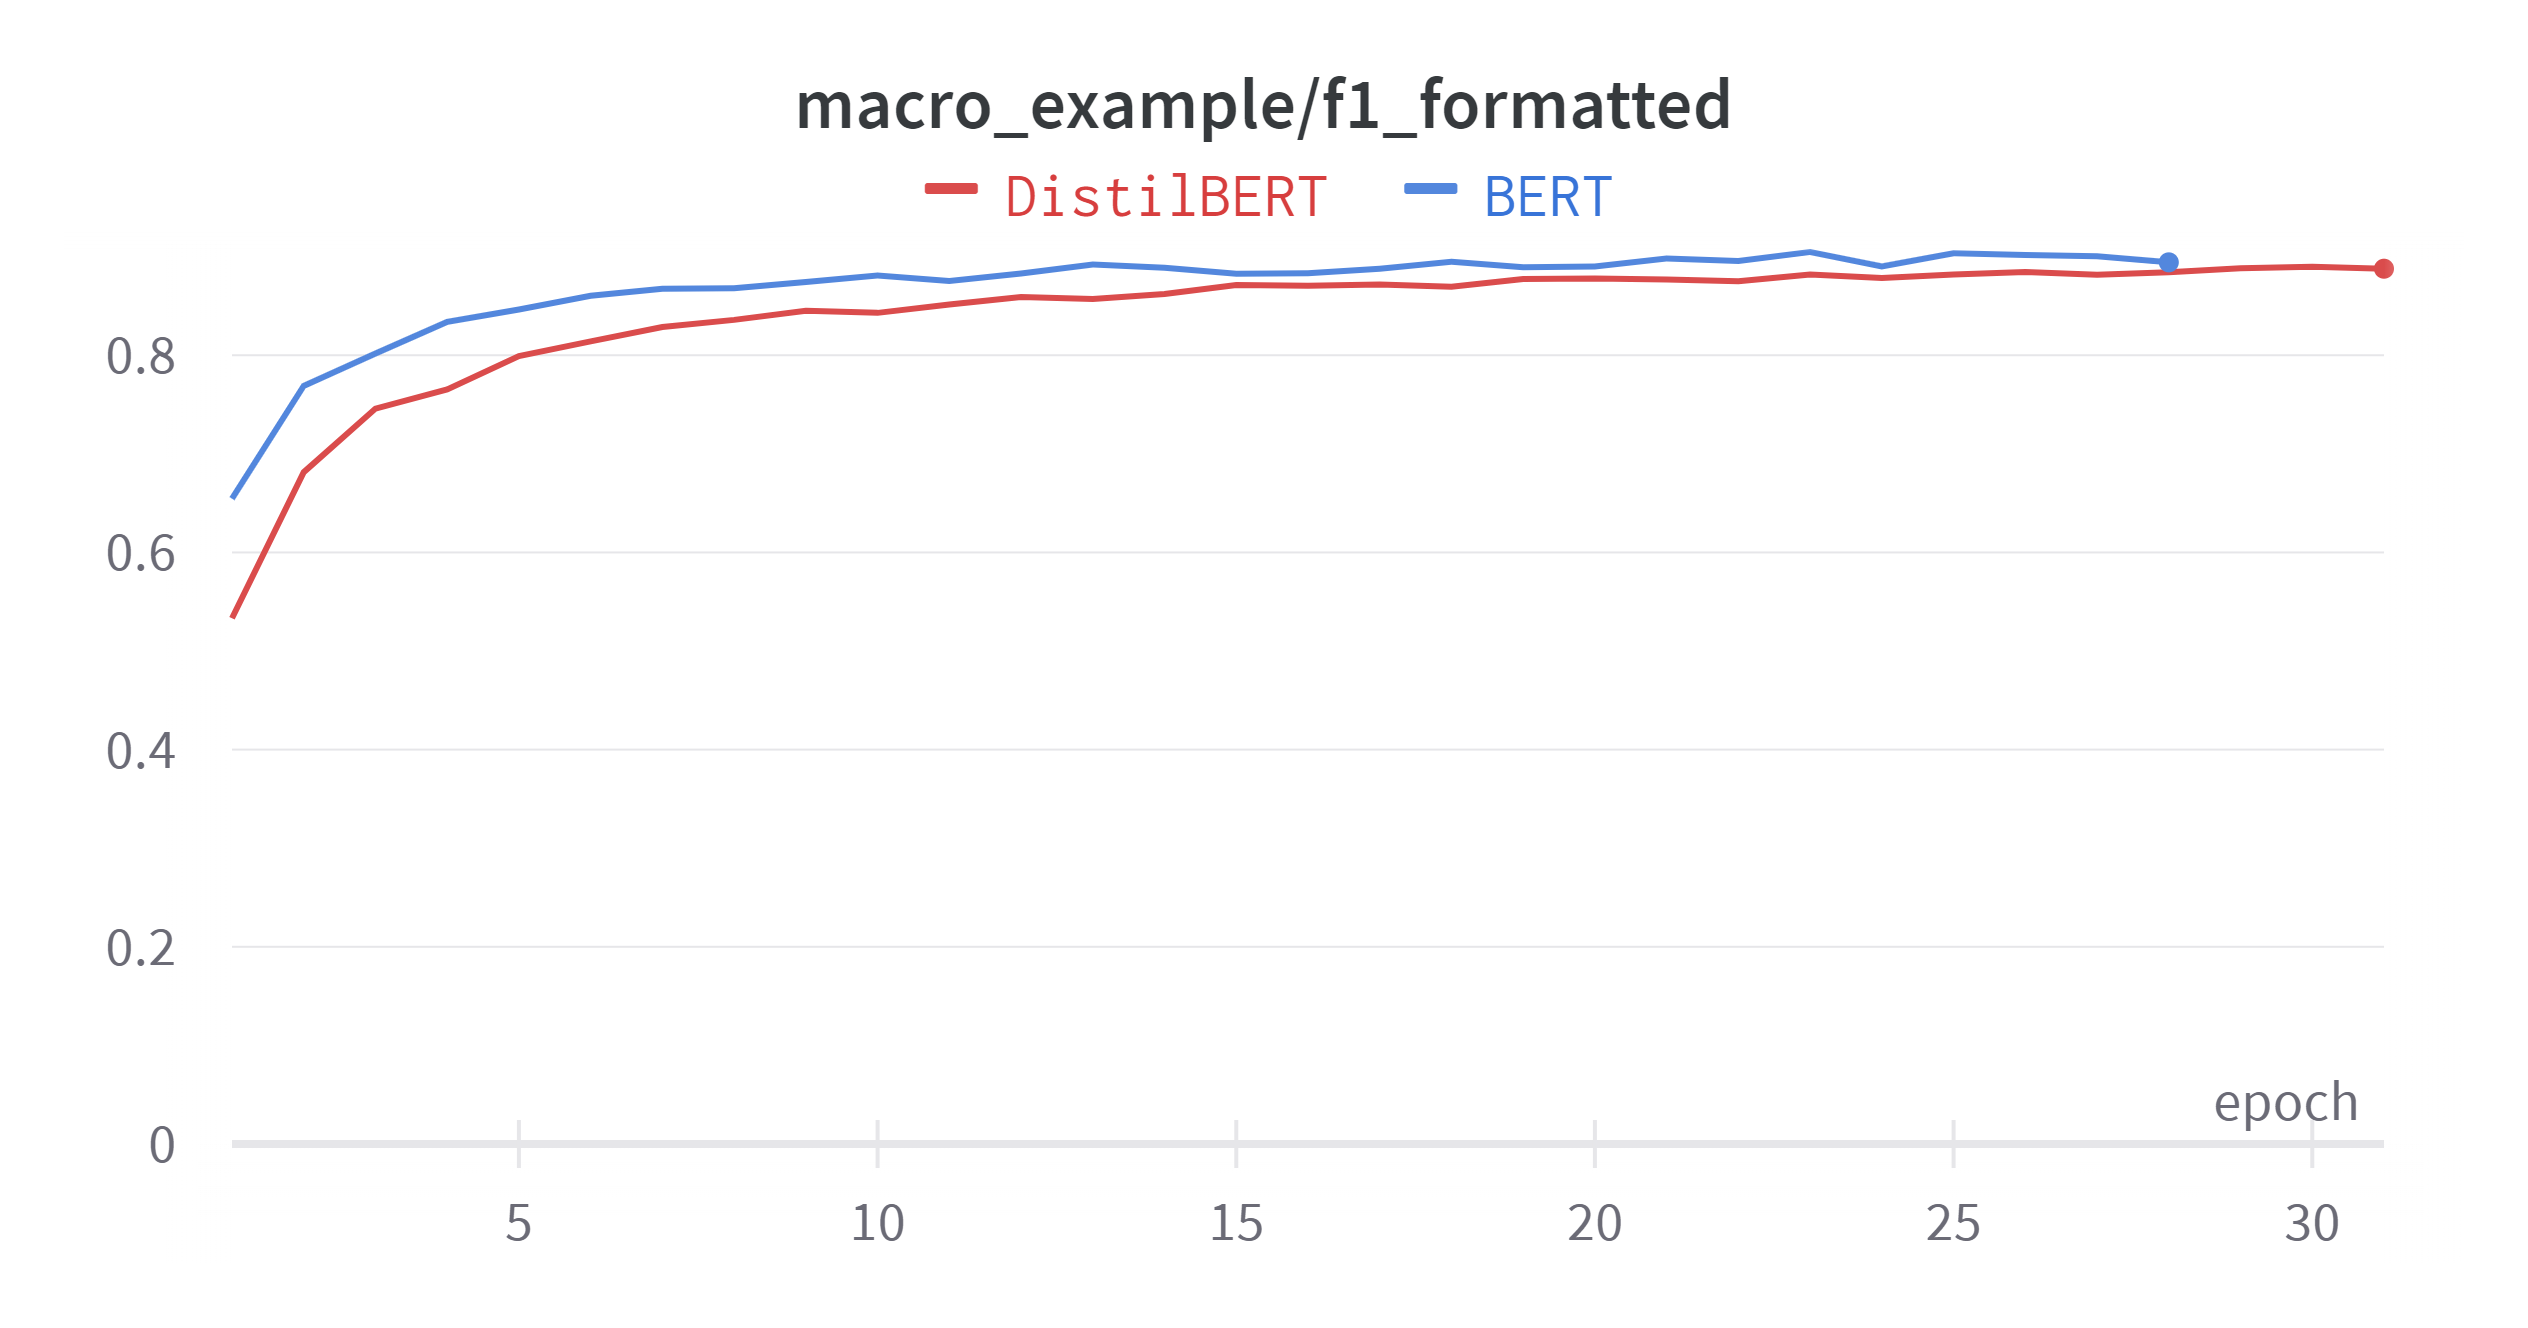
\includegraphics[width=.8\linewidth]{figures/wandb_bbn_baseline_distilbert_vs_bert.png}
    \caption{Baseline DistilBERT vs Baseline BERT in terms of \textit{macro f1 examples} on the dev set of BBN.}
    \label{fig:wandb_bbn_baseline_distilbert_vs_bert}
\end{figure}

The trends of KENN-based models compared to the baseline when using DistilBERT and BERT are available in Figures~\ref{fig:wandb_bbn_kenn_distilbert} and \ref{fig:wandb_bbn_kenn_bert}, respectively. Looking at the graphs, we can make the same observation done for FIGER: the logical knowledge gives an initial boost only when using DistilBERT. Moving on to BERT, except Bottom Up, which has a slower start, the other models have very similar training trends.

\begin{figure}[bth]
    \centering
    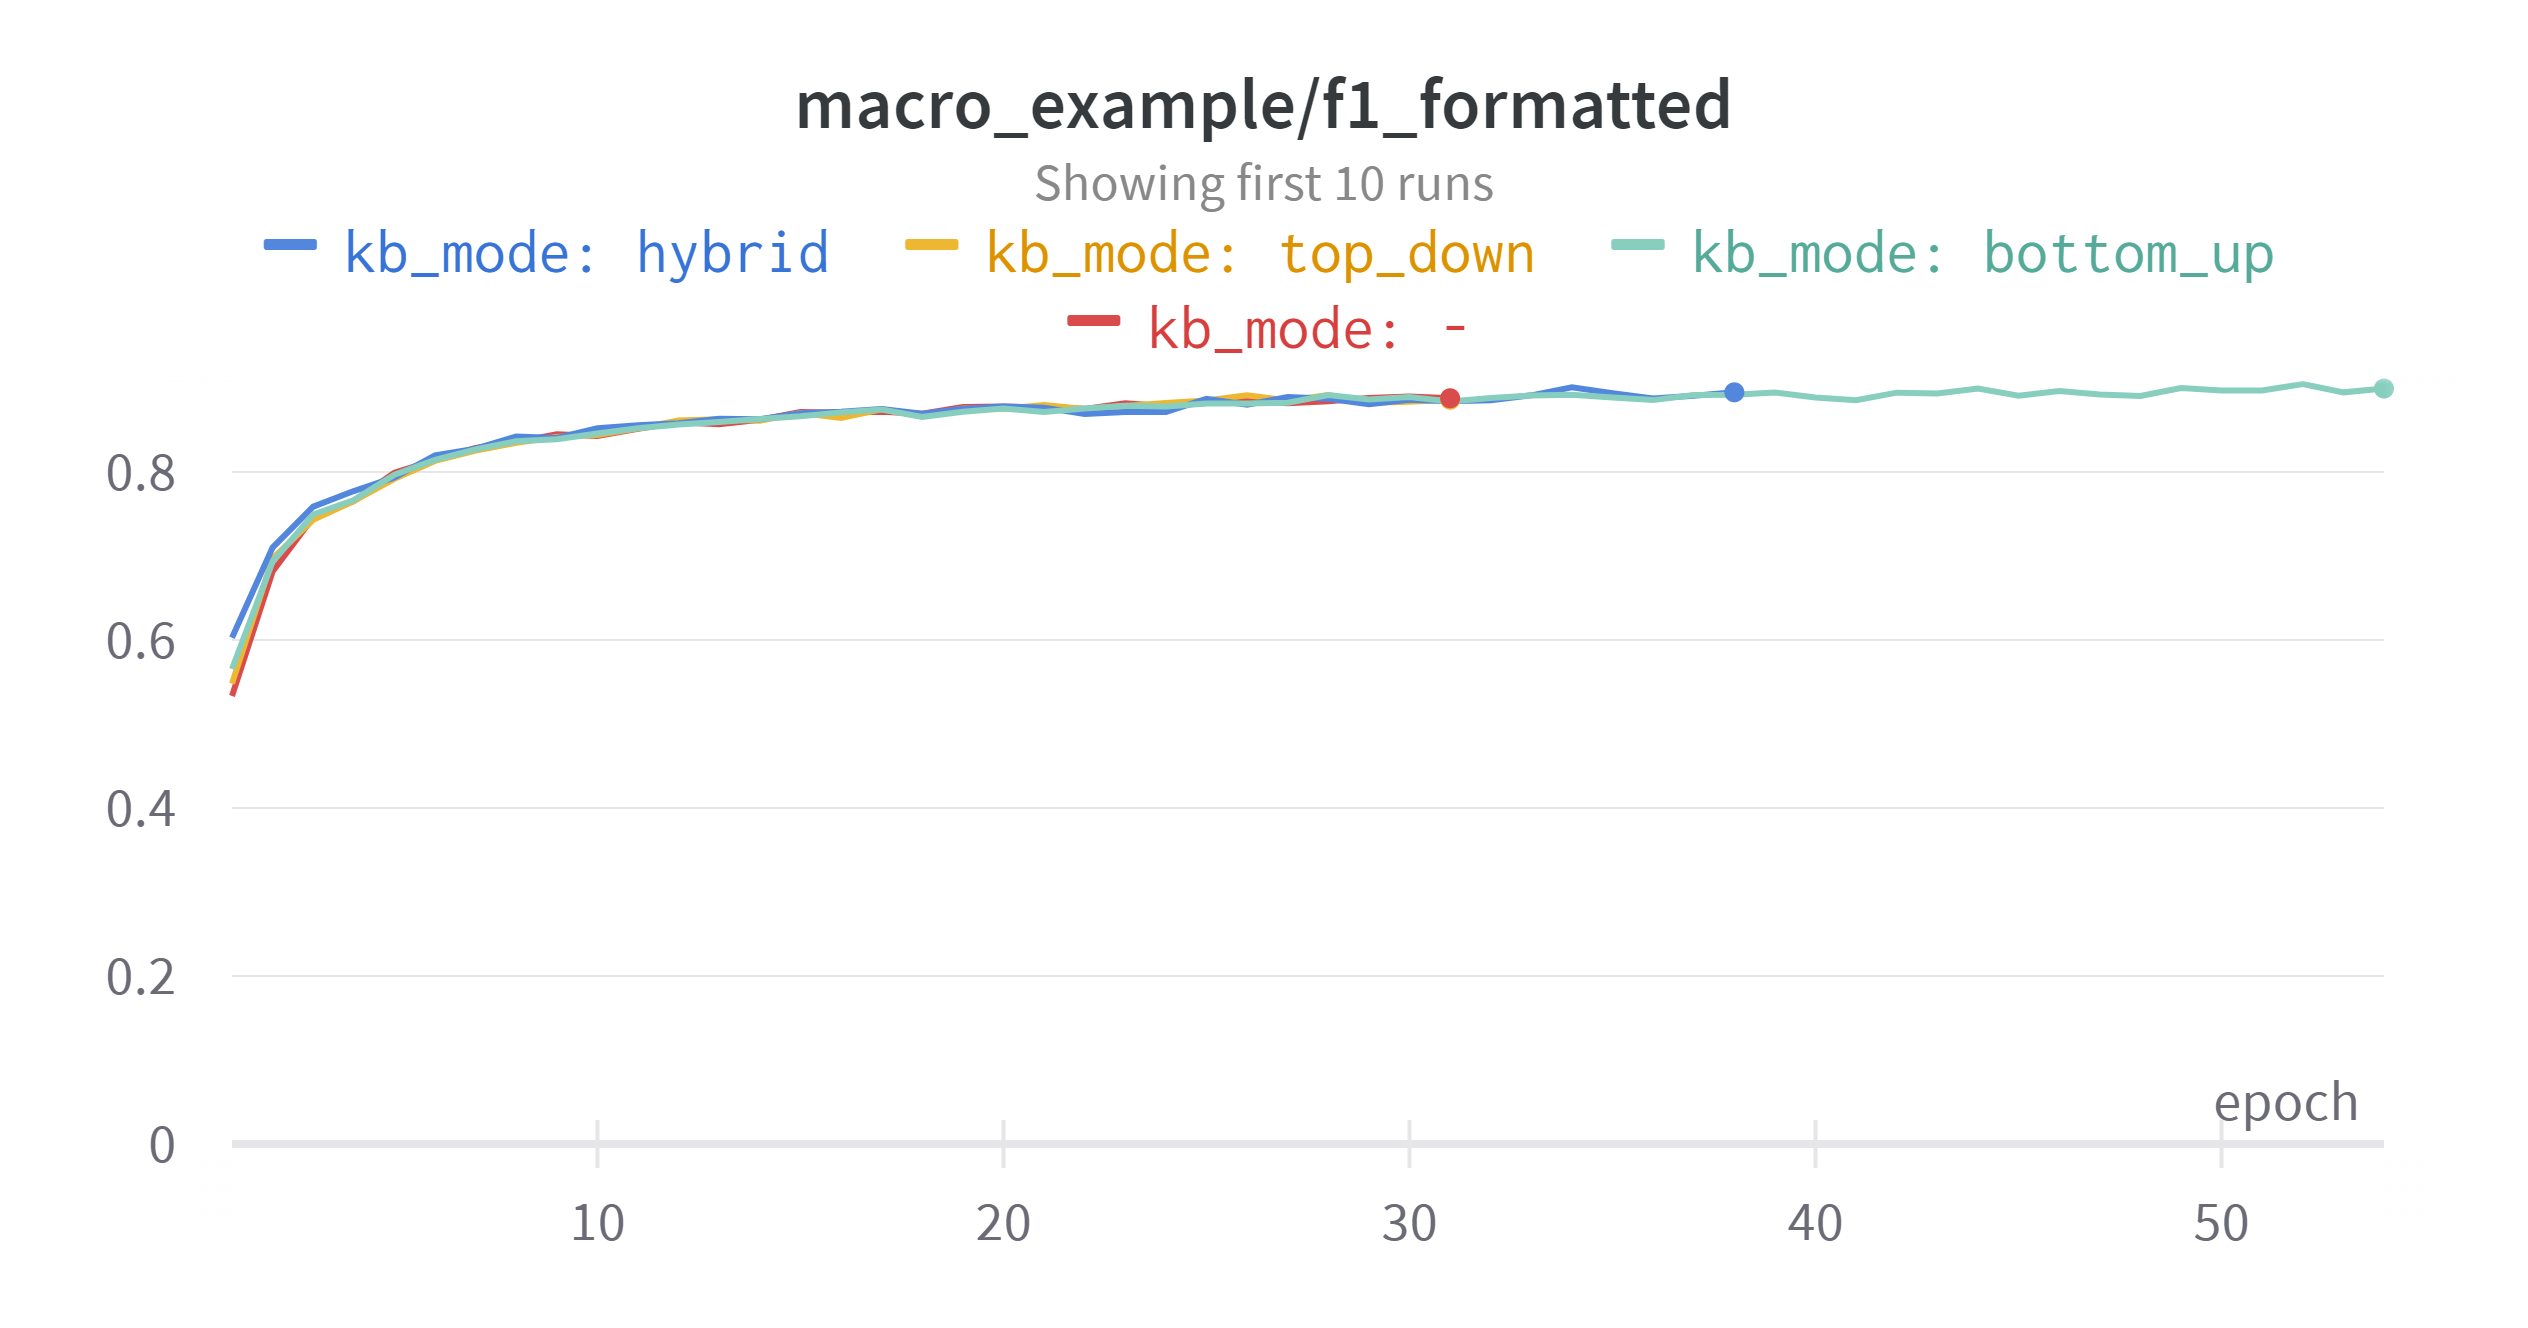
\includegraphics[width=.8\linewidth]{figures/wandb_bbn_kenn_distilbert.png}
    \caption{Baseline DistilBERT vs KENN DistilBERT in terms of \textit{macro f1 examples} on the dev set of BBN.}
    \label{fig:wandb_bbn_kenn_distilbert}
\end{figure}

\begin{figure}[bth]
    \centering
    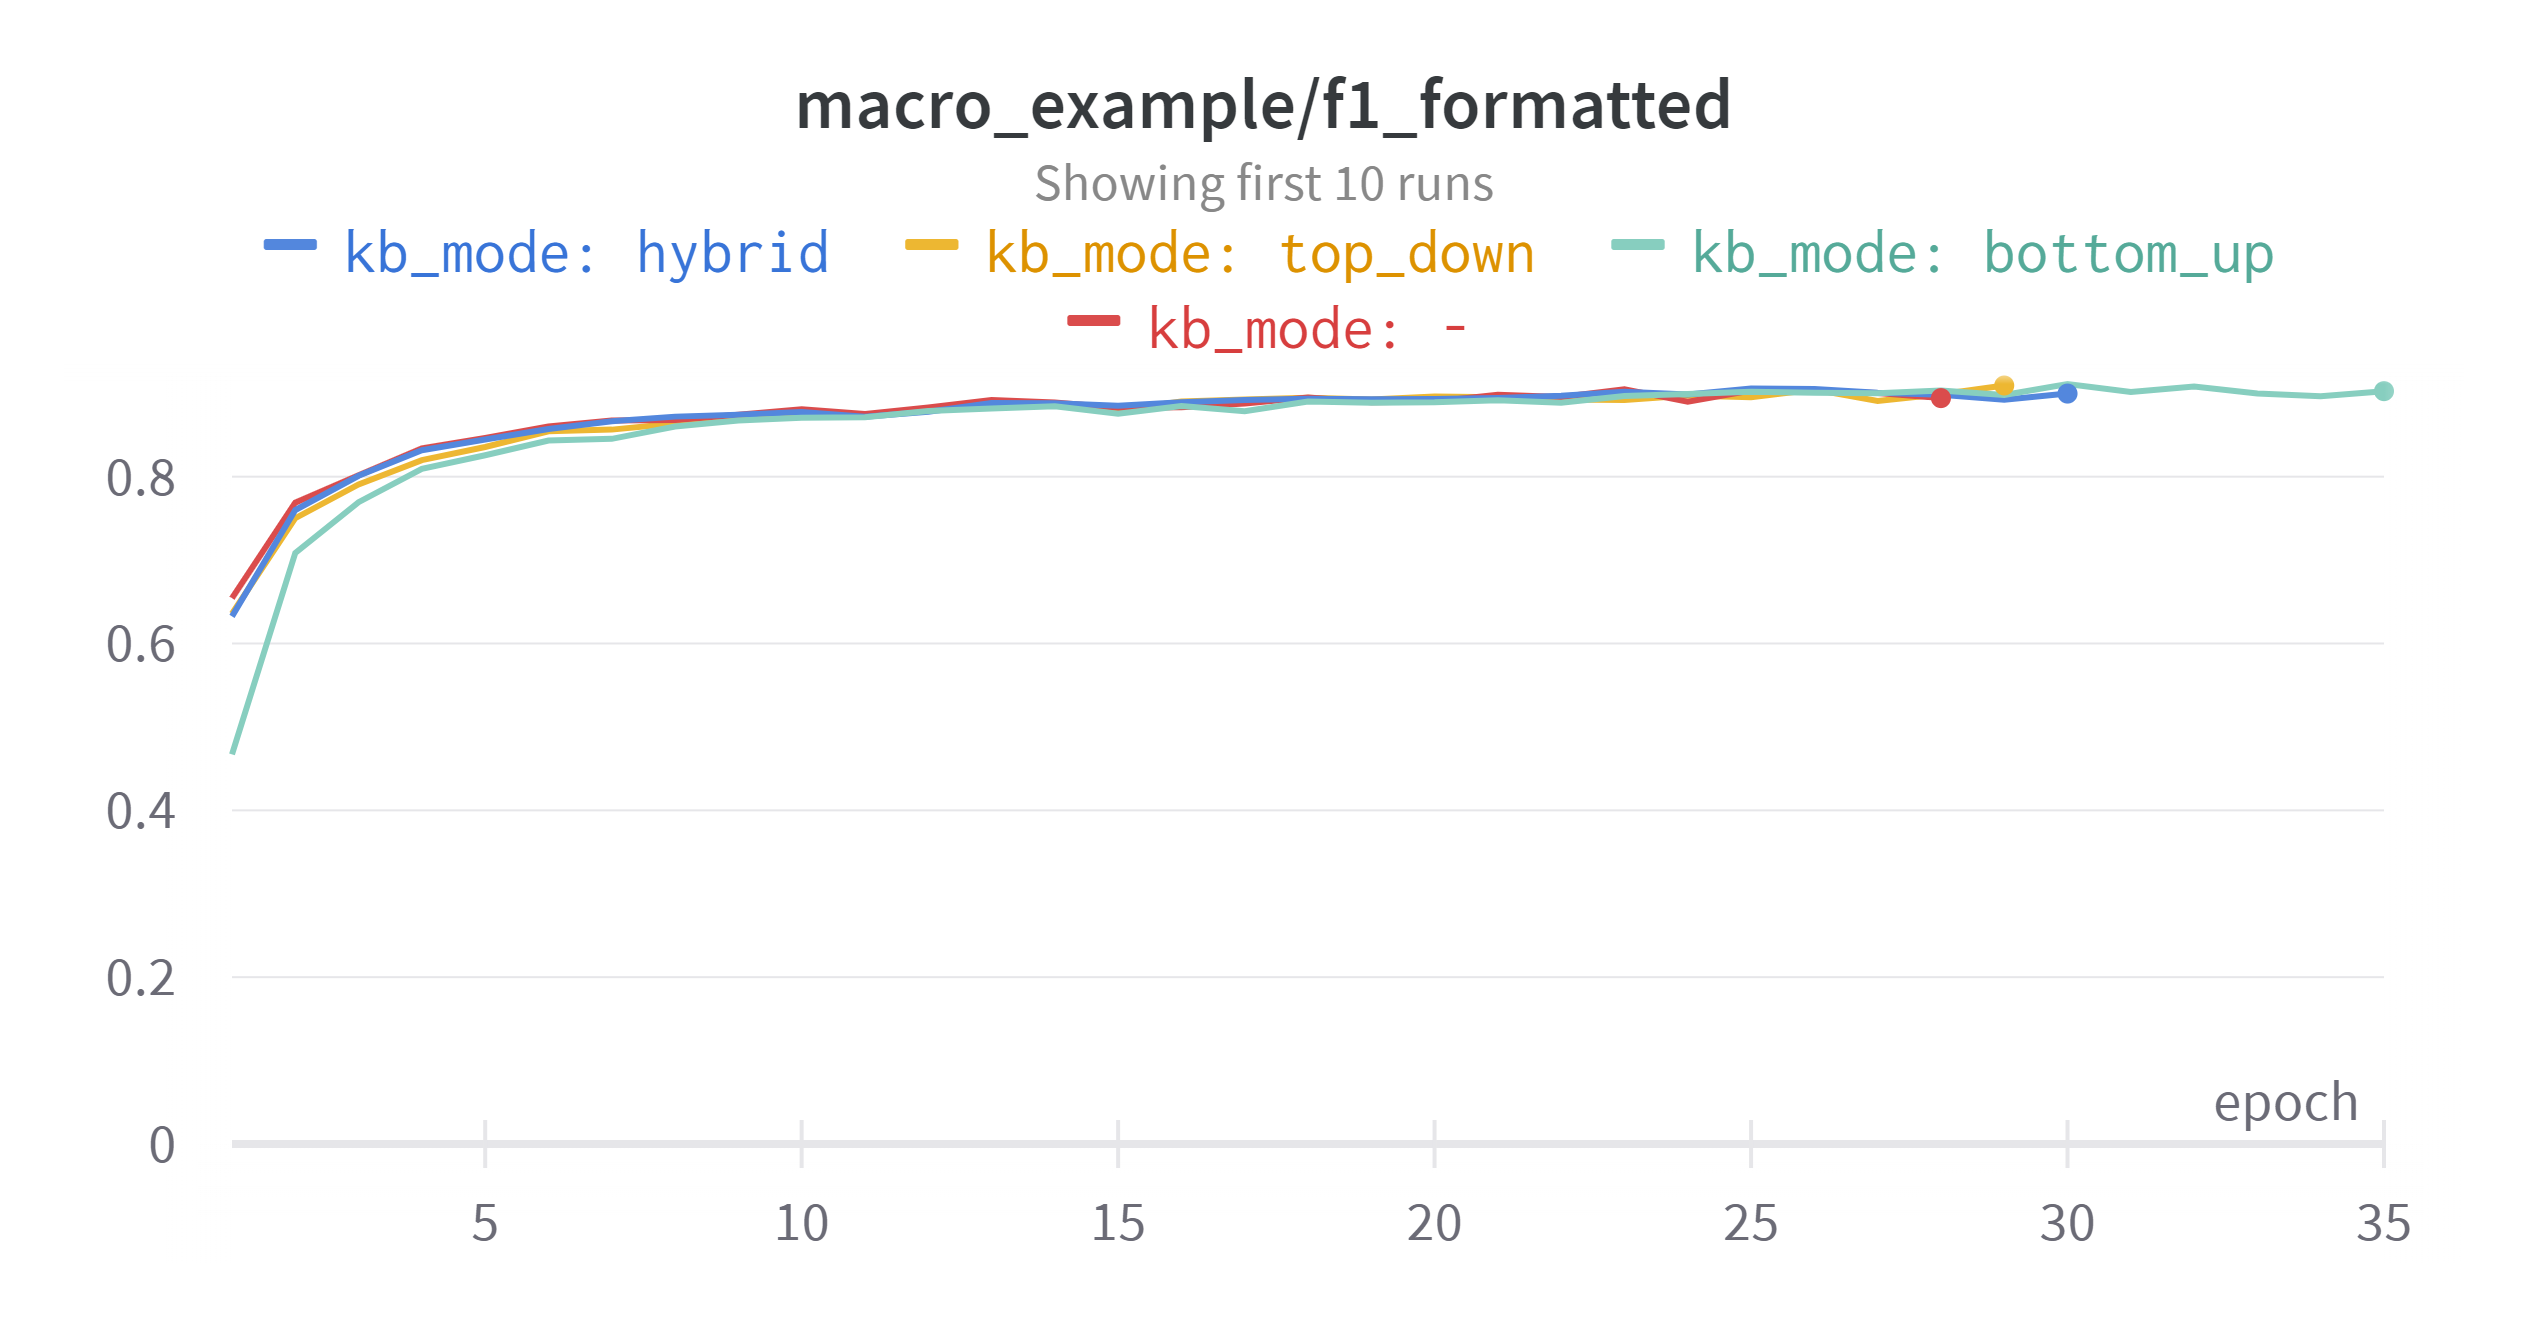
\includegraphics[width=.8\linewidth]{figures/wandb_bbn_kenn_bert.png}
    \caption{Baseline BERT vs KENN BERT in terms of \textit{macro f1 examples} on the dev set of BBN.}
    \label{fig:wandb_bbn_kenn_bert}
\end{figure}

\subsubsection{Conclusion}
The results obtained on the two datasets highlighted that the benefits of the logical knowledge are visible only in the early stage of the DistilBERT-based models. The fact that KENN worsened the performance of the BERT-based models was quite unexpected. Except for the Top Down mode, it seems that the injection of logical knowledge disturbed the learning process of the other models, especially at the beginning of the training. An explanation for this behavior can be found in the words of KENN's authors, which said that KENN has more difficulties when integrated into neural networks that are already capable to satisfy the provided clauses, since any bias is introduced towards their satisfaction~\cite{daniele2021neural}.

In our case, we observed that the performance of the baseline model was substantially improved when using BERT. For this reason, it may be possible that BERT, which provides a richer text representation than DistilBERT, is already able to implicitly learn from data the hierarchical information without the need for logical knowledge. Furthermore, we can think about the differences between the KB modes to explain why Top Down has higher performance than Bottom Up: while the knowledge provided by a Bottom Up clause could be learned from data (i.e., the model learns that a subtype always co-occur with its supertype), Top Down clauses could introduce more bias into the learning process, thus adding new solutions to the Hypothesis Space as said in~\cite{daniele2021neural}.
\subsection{KENN with multiloss function}
In previous experiments, it has been observed that the pre-KENN network adapts to the presence of KENN regardless of the parameters configuration. From these results comes the intuition to make the pre-KENN network more independent, with the purpose of exploiting the logical knowledge more effectively. To achieve this, the idea is to define a custom multiloss function to simultaneously improve the quality of the pre-KENN and post-KENN predictions.

%\subsubsection{Multiloss function}
The proposed multiloss function is computed by combining the Binary Cross-Entropy (BCE) loss values obtained from the pre-KENN and post-KENN preactivations. To make it possible, the model has been adapted to provide two outputs: one before and one after KENN's layer. The goal is to optimize the post-KENN predictions while preserving a discrete quality of pre-KENN predictions. The final loss is computed by the convex combination of the two losses whose influences are regulated by the parameter $ \alpha $. The resulting formula is the following:

% \begin{gather*}
%     L(y_{pred},y_{true}) = \alpha \cdot BCE(y_{prekenn}, y_{true}) + (1 - \alpha) \cdot BCE(y_{postkenn}, y_{true})
% \end{gather*}

\begin{gather*}
    L(Y, Y', Y_{t}) = \alpha \cdot BCE(Y, Y_{t}) + (1 - \alpha) \cdot BCE(Y', Y_{t})
\end{gather*}
where $Y$ denotes the pre-KENN predictions, $Y'$ the post-KENN predictions, and $Y_{t}$ the values of the ground truth.


\subsubsection{Setup}
The models involved in this experiment are trained following the \textit{Setup B}. The configuration of the other parameters is the following:
\begin{itemize}
    \item \textbf{KB modes:} Bottom Up and Top Down
    \item \textbf{initial clause weights:} 0.5 and variable\footnote{With the term ``variable" we mean that each clause can be initialized with a different value. The original implementation of KENN did not contemplate this possibility when setting clause weights as learnable parameters, so we introduced a small modification to make it possible.}
    \item \textbf{learnable clause weights}
    \item \textbf{encoder:} DistilBERT and BERT, with adapters
    \item \textbf{loss function:} multiloss with $\alpha = 0.5$
\end{itemize}
The total number of configurations obtained by varying these parameters is 8. Since the pre-KENN network is expected to be less influenced by KENN, the clause weights are set as learnable parameters with small initial values to start with a soft influence and let the network establish the relevance of each clause. Indeed, the choice of learnable clause weights allows us to study the weight evolution during the epochs and determine which are the most useful and the least useful clauses. Furthermore, for each clause, the types that are the antecedents of an implication rule (i.e., the types that propagate the information and uniquely characterize the used KBs) have been studied to look for some recurring behavioral patterns. The \textit{Hybrid} mode is excluded from this study because it involves the same clauses of \textit{Bottom Up} and \textit{Top Down}, but with the addition of noise due to the presence of conflicts. For this reason, it would not have been possible to carry out an accurate analysis.

\subsubsection{Results on FIGER}
\paragraph{DistilBERT}
The results obtained using DistilBERT as encoder show some very interesting behaviors of the clause weights. Starting from the Bottom Up, if we look at the distribution of final clause weights in Figure~\ref{fig:weight_distrib_distilbert_figer_bu_multiloss} we can see that almost every weight decreases its initial value. This attitude is not observable in Figure~\ref{fig:weight_distrib_distilbert_figer_bu_learnable} when using KENN with a standard loss and learnable weights. If we look at the figure, we can see widely different results since almost every weight increases its starting value. The same trend is detectable in the Top Down mode, as shown in Figure~\ref{fig:weight_distrib_distilbert_figer_td}.

\begin{figure}[bth]
     \centering
     \begin{subfigure}[b]{0.45\textwidth}
         \centering
         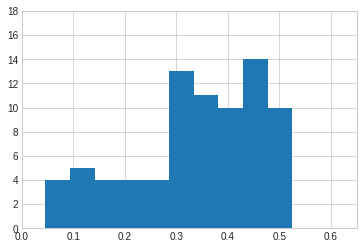
\includegraphics[width=\textwidth]{figures/weight_distrib_distilbert_figer_bu_multiloss.png}
         \caption{Multiloss model - Epoch 55 (563K examples)}
         \label{fig:weight_distrib_distilbert_figer_bu_multiloss}
     \end{subfigure}
     \hspace{10px}
     \begin{subfigure}[b]{0.45\textwidth}
         \centering
         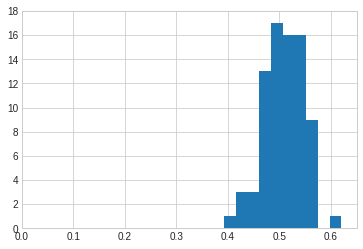
\includegraphics[width=\textwidth]{figures/weight_distrib_distilbert_figer_bu_learnable.png}
         \caption{Standard loss model - Epoch 42 (430K examples)}
         \label{fig:weight_distrib_distilbert_figer_bu_learnable}
     \end{subfigure}
    \caption{Distributions of the final learned clause weights for the Bottom Up KB mode using DistilBERT-based models - FIGER}
    \label{fig:weight_distrib_distilbert_figer_bu}
\end{figure}

\begin{figure}[bth]
     \centering
     \begin{subfigure}[b]{0.45\textwidth}
         \centering
         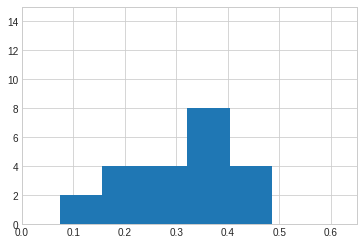
\includegraphics[width=\textwidth]{figures/weight_distrib_distilbert_figer_td_multiloss.png}
         \caption{Multiloss model - Epoch 42 (430K examples)}
         \label{fig:weight_distrib_distilbert_figer_td_multiloss}
     \end{subfigure}
     \hspace{10px}
     \begin{subfigure}[b]{0.45\textwidth}
         \centering
         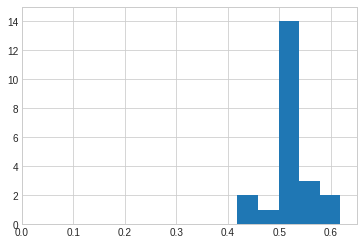
\includegraphics[width=\textwidth]{figures/weight_distrib_distilbert_figer_td_learnable.png}
         \caption{Standard loss model - Epoch 39 (399K examples)}
         \label{fig:weight_distrib_distilbert_figer_td_learnable}
     \end{subfigure}
    \caption{Distributions of the final learned clause weights for the Top Down KB mode using DistilBERT-based models - FIGER}
    \label{fig:weight_distrib_distilbert_figer_td}
\end{figure}


Moving on to the analysis of the types involved in the clauses we can observe an unexpected behavior. For both Bottom Up and Top Down modes, this study intercepts a remarkable fact: the more a type occurs in the training set, the lower the final weight of its clause. The few clauses that preserve a high weight are those whose antecedents are the rarest in the dataset. Starting from the Bottom Up mode, we can see in Figure~\ref{fig:weight_freq_distilbert_figer_bu_multiloss} a graph showing the relation between the final weight and the frequency of each type S. Looking at the figure, we can clearly observe that there is a strong correlation between weight and frequency. Indeed, the correlation coefficient is -0.77. The Top Down mode (Figure~\ref{fig:weight_freq_distilbert_figer_td_multiloss}) also presents a negative correlation, this time of -0.68 with respect to the frequencies of types F.
%This behavior may be explained by the fact that KENN introduces too much noise to types that the network can already predict discretely without the use of knowledge. 

\begin{figure}[bth]
     \centering
     \begin{subfigure}[b]{0.7\textwidth}
         \centering
         \includegraphics[width=\textwidth]{figures/weight_freq_distilbert_figer_bu_multiloss.png}
         \caption{Bottom Up - Epoch 55 (563K examples)}
         \label{fig:weight_freq_distilbert_figer_bu_multiloss}
         \vspace{10px}
     \end{subfigure}
     \begin{subfigure}[b]{0.7\textwidth}
         \centering
         \includegraphics[width=\textwidth]{figures/weight_freq_distilbert_figer_td_multiloss.png}
         \caption{Top Down - Epoch 42 (430K examples)}
         \label{fig:weight_freq_distilbert_figer_td_multiloss}
     \end{subfigure}
    \caption{Relation between types frequency (log scale) and final clause weights of multiloss models using DistilBERT - FIGER}
    \label{fig:weight_freq_distilbert_figer}
\end{figure}

By inspecting the weight evolution over the epochs, it emerged that the clause weights keep decreasing until the last epoch, but it is not known for how long they would have continued. To observe in advance the effect of higher epochs and see if some clauses would have reached a weight close to zero, new models were trained starting from variable weights assigned with respect to the frequency of the antecedents of each clause. Clauses involving popular types were assigned a weight of 0.2, while the others kept a weight of 0.5. The weight assignment is based on a frequency threshold of 70K for Bottom Up and 50K for Top Down\footnote{the values are chosen by observing the graphs, without formalizing a mathematical criterion}. The results of these runs are shown in Figure~\ref{fig:weight_freq_distilbert_figer_bu_multiloss_variable} and Figure~\ref{fig:weight_freq_distilbert_figer_td_multiloss_variable} for Bottom Up and Top Down, respectively. As we can see, most clause weights decreased their values even when starting from lower initial values.
%However, by analyzing the weight evolution, it emerged that their decrease over the epochs was slowed down. The reason for this fact is that clauses now have less influence on the final prediction, so they are penalized in a minor way by the loss function.

\begin{figure}[bth]
     \centering
     \begin{subfigure}[b]{0.7\textwidth}
         \centering
         \includegraphics[width=\textwidth]{figures/weight_freq_distilbert_figer_bu_multiloss_variable.png}
         \caption{Bottom Up - Epoch 71 (727K examples)}
         \label{fig:weight_freq_distilbert_figer_bu_multiloss_variable}
         \vspace{10px}
     \end{subfigure}
     \begin{subfigure}[b]{0.7\textwidth}
         \centering
         \includegraphics[width=\textwidth]{figures/weight_freq_distilbert_figer_td_multiloss_variable.png}
         \caption{Top Down - Epoch 42 (430K examples)}
         \label{fig:weight_freq_distilbert_figer_td_multiloss_variable}
     \end{subfigure}
    \caption{Relation between types frequency (log scale) and final clause weights of multiloss models using DistilBERT and \textit{variable} clause weights - FIGER}
    \label{fig:weight_freq_distilbert_figer_variable}
\end{figure}

\paragraph{BERT}
The experiments performed using BERT showed an identical behavior. The results obtained with weights set to 0.5 for every clause are shown in Figure~\ref{fig:weight_freq_bert_figer}. The correlation between weight and frequency is similar (-0.76 in Bottom Up, -0.74 in Top Down) as well as the weight evolution during the epochs. The only difference with respect to DistilBERT is that BERT needs fewer epochs to converge, so its weights have decreased less as it performed fewer backward propagation operations. Much lower weights are reached when using the setup with variable weights as reported in Figure~\ref{fig:weight_freq_bert_figer_variable}.

\begin{figure}[bth]
     \centering
     \begin{subfigure}[b]{0.7\textwidth}
         \centering
         \includegraphics[width=\textwidth]{figures/weight_freq_bert_figer_bu_multiloss.png}
         \caption{Bottom Up - Epoch 35 (358K training examples)}
         \label{fig:weight_freq_bert_figer_bu_multiloss}
         \vspace{10px}
     \end{subfigure}
     \begin{subfigure}[b]{0.7\textwidth}
         \centering
         \includegraphics[width=\textwidth]{figures/weight_freq_bert_figer_td_multiloss.png}
         \caption{Top Down - Epoch 35 (358K training examples)}
         \label{fig:weight_freq_bert_figer_td_multiloss}
     \end{subfigure}
    \caption{Relation between types frequency (log scale) and final clause weights of multiloss models using BERT - FIGER}
    \label{fig:weight_freq_bert_figer}
\end{figure}

\begin{figure}[bth]
     \centering
     \begin{subfigure}[b]{0.7\textwidth}
         \centering
         \includegraphics[width=\textwidth]{figures/weight_freq_bert_figer_bu_multiloss_variable.png}
         \caption{Bottom Up - Epoch 49 (501K training examples)}
         \label{fig:weight_freq_bert_figer_bu_multiloss_variable}
         \vspace{10px}
     \end{subfigure}
     \begin{subfigure}[b]{0.7\textwidth}
         \centering
         \includegraphics[width=\textwidth]{figures/weight_freq_bert_figer_td_multiloss_variable.png}
         \caption{Top Down - Epoch 33 (337K training examples)}
         \label{fig:weight_freq_bert_figer_td_multiloss_variable}
     \end{subfigure}
    \caption{Relation between types frequency (log scale) and final clause weights of multiloss models using BERT and \textit{variable} clause weights - FIGER}
    \label{fig:weight_freq_bert_figer_variable}
\end{figure}


\subsubsection{Results on BBN}
The experiments on BBN were performed directly on BERT. In Figure~\ref{fig:weight_freq_bert_bbn} are represented the graphs of weights and frequencies using the same weight for each clause. The correlation coefficients of the Bottom Up and Top Down modes are -0.73 and -0.55, respectively. The results obtained after repeating the experiments using variable weights are shown in Figure~\ref{fig:weight_freq_bert_bbn_variable}. The weight assignment is based on a frequency threshold of 1700 for Bottom Up and 1500 for Top Down\footnote{the values are chosen by observing the graphs, without formalizing a mathematical criterion}. Looking at the graphs, it is possible to observe that most of the weights continued to decrease.

\begin{figure}
     \centering
     \begin{subfigure}[b]{0.7\textwidth}
         \centering
         \includegraphics[width=\textwidth]{figures/weight_freq_bert_bbn_bu_multiloss.png}
         \caption{Bottom Up - Epoch 28 (286K training examples)}
         \label{fig:weight_freq_bert_bbn_bu_multiloss}
         \vspace{10px}
     \end{subfigure}
     \begin{subfigure}[b]{0.7\textwidth}
         \centering
         \includegraphics[width=\textwidth]{figures/weight_freq_bert_bbn_td_multiloss.png}
         \caption{Top Down - Epoch 19 (194K training examples)}
         \label{fig:weight_freq_bert_bbn_td_multiloss}
     \end{subfigure}
    \caption{Relation between types frequency (log scale) and final clause weights of multiloss models using BERT - BBN}
    \label{fig:weight_freq_bert_bbn}
\end{figure}

\begin{figure}
     \centering
     \begin{subfigure}[b]{0.7\textwidth}
         \centering
         \includegraphics[width=\textwidth]{figures/weight_freq_bert_bbn_bu_multiloss_variable.png}
         \caption{Bottom Up - Epoch 19 (194K training examples)}
         \label{fig:weight_freq_bert_bbn_bu_multiloss_variable}
         \vspace{10px}
     \end{subfigure}
     \begin{subfigure}[b]{0.7\textwidth}
         \centering
         \includegraphics[width=\textwidth]{figures/weight_freq_bert_bbn_td_multiloss_variable.png}
         \caption{Top Down - Epoch 19 (194K training examples)}
         \label{fig:weight_freq_bert_bbn_td_multiloss_variable}
     \end{subfigure}
    \caption{Relation between types frequency (log scale) and final clause weights of multiloss models using BERT and \textit{variable} clause weights - BBN}
    \label{fig:weight_freq_bert_bbn_variable}
\end{figure}



\subsubsection{Conclusion}
The multiloss experiments showed that the pre-KENN network suffers the presence of some logical clauses when it is forced to not adapt its predictions to KENN. In particular, it has been possible to see that the learning process penalized clauses involving the most frequent types much more than the others. This behavior can be motivated by the fact that if a network sees a lot of instances labeled with some types, then it becomes able to correctly classify them without needing logical knowledge. For this reason, it seems that the action of KENN on frequent types is seen as noise added to the final predictions. Conversely, the enhancement of rarer types is not penalized by the learning process, so logical clauses seem to be helpful for the network when few examples labeled with those types are available. For this reason, using a multiloss setup could be a reasonable choice to exploit logical knowledge only where needed, thus avoiding having side effects on the types that are easier to predict.


\subsection{Test set evaluation} \label{test_evaluation}
The models chosen for the test set evaluation come from the multiloss experiments. Based on \textit{Setup B}, they have the following configuration:
\begin{itemize}
    \item \textbf{KB modes:} Bottom Up and Top Down
    \item \textbf{initial clause weights:} 0.5 and variable
    \item \textbf{learnable clause weights}
    \item \textbf{encoder:} BERT with adapters
    \item \textbf{loss function:} multiloss with $\alpha = 0.5$
\end{itemize}
% scelta modelli
The choice of the multiloss setup has the following reasons derived from the experimental results:
\begin{enumerate}
    \item When using a standard loss setup, the pre-KENN network adapts its predictions to the presence of KENN and achieves results that are very similar to the baseline ones. This means that KENN-based models can be seen as simple baseline models that have had different evolutions due to the noise introduced by KENN.
    \item When using a multiloss setup, the pre-KENN network avoids the adaptation thanks to the pre-KENN loss. The final clause weights will ensure that the network only uses KENN when it really needs it.
    \item The choice of variable clause weights may emphasize the effect of the multiloss on final weights, thus producing models in which the influence of KENN is slightly different.
\end{enumerate}
The test set has been evaluated using the metrics of \textit{macro f1 examples} and \textit{macro f1 classes}. The inference rules used to compute the final predictions are the \textit{threshold} and \textit{threshold or max}.

\paragraphn{Results on FIGER}
Table~\ref{tab:performance_figer} shows the results obtained on FIGER. If we look at the performance with the \textit{threshold} inference, we can see that the Top Down mode is the best in every metric. With respect to the baseline model, it gains 0.0151 on \textit{macro f1 examples} and 0.0108 on \textit{macro f1 classes}. 

KENN-based models become even more competitive when using the \textit{threshold or max} inference. In this case, the metrics obtained by Bottom Up and Top Down are quite similar. The best performance on \textit{macro f1 examples} and \textit{macro f1 classes} are reached by Bottom Up and Top Down by gaining 0.0181 and 0.0137, respectively, over the baseline. Note that by changing the inference rule, Bottom Up and Top Down increase their \textit{macro examples f1} much more than the baseline.

\begin{table}[H]
\centering
\caption{Performance of the baseline and KENN multiloss models on the test set - FIGER}
\label{tab:performance_figer}
\resizebox{\columnwidth}{!}{\begin{tabular}{cc|ccc|ccc|}
\cline{3-8}
\textbf{} &  & \multicolumn{3}{c|}{\textbf{Macro examples}} & \multicolumn{3}{c|}{\textbf{Macro classes}} \\ \hline
\multicolumn{1}{|c|}{\textbf{KB mode}} & \textbf{Inference} & \textbf{P} & \textbf{R} & \textbf{F1} & \textbf{P} & \textbf{R} & \textbf{F1} \\ \hline
\noalign{\hrule height 1pt}
\multicolumn{1}{|c|}{- (baseline)} & threshold & 0.7884 & 0.8601 & 0.8227 & 0.2305 & 0.2526 & 0.2410 \\ \hline
\multicolumn{1}{|c|}{\begin{tabular}[c]{@{}c@{}}Bottom Up\\ (variable weights)\end{tabular}} & threshold & 0.7631 & 0.8501 & 0.8043 & 0.2171 & 0.2459 & 0.2306 \\ \hline
\multicolumn{1}{|c|}{Bottom Up} & threshold & 0.7854 & 0.8611 & 0.8215 & 0.2343 & 0.2630 & 0.2478 \\ \hline
\multicolumn{1}{|c|}{\begin{tabular}[c]{@{}c@{}}Top Down\\ (variable weights)\end{tabular}} & threshold & 0.7560 & 0.8627 & 0.8058 & 0.2157 & 0.2445 & 0.2292 \\ \hline
\multicolumn{1}{|c|}{Top Down} & threshold & \textbf{0.7997} & \textbf{0.8796} & \textbf{0.8378} & \textbf{0.2404} & \textbf{0.2643} & \textbf{0.2518} \\ \hline
\noalign{\hrule height 1pt}
\multicolumn{1}{|c|}{- (baseline)} & \begin{tabular}[c]{@{}c@{}}threshold\\ or max\end{tabular} & 0.8008 & 0.8699 & 0.8339 & 0.2355 & 0.2542 & 0.2445 \\ \hline
\multicolumn{1}{|c|}{\begin{tabular}[c]{@{}c@{}}Bottom Up\\ (variable weights)\end{tabular}} & \begin{tabular}[c]{@{}c@{}}threshold\\ or max\end{tabular} & 0.7950 & 0.8795 & 0.8351 & 0.2156 & 0.2492 & 0.2312 \\ \hline
\multicolumn{1}{|c|}{Bottom Up} & \begin{tabular}[c]{@{}c@{}}threshold\\ or max\end{tabular} & \textbf{0.8174} & 0.8898 & \textbf{0.8520} & 0.2327 & \textbf{0.2718} & 0.2507 \\ \hline
\multicolumn{1}{|c|}{\begin{tabular}[c]{@{}c@{}}Top Down\\ (variable weights)\end{tabular}} & \begin{tabular}[c]{@{}c@{}}threshold\\ or max\end{tabular} & 0.7773 & 0.8831 & 0.8268 & 0.2298 & 0.2518 & 0.2403 \\ \hline
\multicolumn{1}{|c|}{Top Down} & \begin{tabular}[c]{@{}c@{}}threshold\\ or max\end{tabular} & 0.8139 & \textbf{0.8903} & 0.8504 & \textbf{0.2495} & 0.2676 & \textbf{0.2582} \\ \hline
\end{tabular}}
\end{table}



\paragraphn{Results on BBN}
% threshold: top down i due migliori
In Table~\ref{tab:performance_bbn} we can find the results obtained on BBN. Except for the \textit{macro classes} metrics, the best results are achieved by both the Top Down modes regardless of the inference rule. This time, in constrast to FIGER, the baseline and KENN-based models have a similar boost on the performance when moving from \textit{threshold} to \textit{threshold or max} inference.

\begin{table}[H]
\centering
\caption{Performance of the baseline and KENN multiloss models on the test set - BBN}
\label{tab:performance_bbn}
\resizebox{\columnwidth}{!}{\begin{tabular}{cc|ccc|ccc|}
\cline{3-8}
\textbf{} &  & \multicolumn{3}{c|}{\textbf{Macro examples}} & \multicolumn{3}{c|}{\textbf{Macro classes}} \\ \hline
\multicolumn{1}{|c|}{\textbf{KB mode}} & \textbf{Inference} & \textbf{P} & \textbf{R} & \textbf{F1} & \textbf{P} & \textbf{R} & \textbf{F1} \\ \hline
\noalign{\hrule height 1pt}
\multicolumn{1}{|c|}{- (baseline)} & threshold & 0.7428 & 0.8197 & 0.7793 & \textbf{0.4893} & 0.4981 & \textbf{0.4937} \\ \hline
\multicolumn{1}{|c|}{\begin{tabular}[c]{@{}c@{}}Bottom Up\\ (variable weights)\end{tabular}} & threshold & 0.7489 & 0.8222 & 0.7839 & 0.4783 & 0.4947 & 0.4864 \\ \hline
\multicolumn{1}{|c|}{Bottom Up} & threshold & 0.7417 & 0.8149 & 0.7766 & 0.4682 & \textbf{0.5099} & 0.4882 \\ \hline
\multicolumn{1}{|c|}{\begin{tabular}[c]{@{}c@{}}Top Down\\ (variable weights)\end{tabular}} & threshold & 0.7540 & 0.8279 & 0.7892 & 0.4825 & 0.4990 & 0.4906 \\ \hline
\multicolumn{1}{|c|}{Top Down} & threshold & \textbf{0.7551} & \textbf{0.8297} & \textbf{0.7906} & 0.4560 & 0.4770 & 0.4663 \\ \hline
\noalign{\hrule height 1pt}
\multicolumn{1}{|c|}{- (baseline)} & \begin{tabular}[c]{@{}c@{}}threshold\\ or max\end{tabular} & 0.7531 & 0.8272 & 0.7884 & 0.4730 & 0.5007 & 0.4865 \\ \hline
\multicolumn{1}{|c|}{\begin{tabular}[c]{@{}c@{}}Bottom Up\\ (variable weights)\end{tabular}} & \begin{tabular}[c]{@{}c@{}}threshold\\ or max\end{tabular} & 0.7617 & 0.8305 & 0.7946 & 0.4607 & 0.5019 & 0.4804 \\ \hline
\multicolumn{1}{|c|}{Bottom Up} & \begin{tabular}[c]{@{}c@{}}threshold\\ or max\end{tabular} & 0.7516 & 0.8216 & 0.7851 & 0.4589 & 0.5125 & 0.4842 \\ \hline
\multicolumn{1}{|c|}{\begin{tabular}[c]{@{}c@{}}Top Down\\ (variable weights)\end{tabular}} & \begin{tabular}[c]{@{}c@{}}threshold\\ or max\end{tabular} & 0.7649 & 0.8353 & 0.7986 & \textbf{0.4775} & \textbf{0.5131} & \textbf{0.4947} \\ \hline
\multicolumn{1}{|c|}{Top Down} & \begin{tabular}[c]{@{}c@{}}threshold\\ or max\end{tabular} & \textbf{0.7676} & \textbf{0.8387} & \textbf{0.8016} & 0.4477 & 0.4917 & 0.4687 \\ \hline
\end{tabular}}
\end{table}

\paragraphn{Test set considerations}
% 18/24 le modalità top down sono andate meglio -> motivi? la rete fa meno fatica a classificare i tipi coarse, proababile sia quello
The configurations involving the Top Down mode are the ones that achieved the best results. If we group the results of both datasets by the inference rule and consider the performance of Top Down with and without variable weights together, we can see that this KB mode reached the highest metric in 18 out of 24 cases\footnote{$|metrics| \times |inference \; rules| \times |datasets| = 6 \times 2 \times 2 = 24$ metrics}. The reason for these results may be that is known that the classification of a supertype (i.e., the antecedent of a Top Down clause) is generally easier than the classification of a subtype, so the boost produced by KENN seems to be more effective when propagated from supertypes to subtypes. However, this aspect needs to be further investigated and has been left for future work.

A final consideration can be made on the test sets as they have significant differences compared to the training sets (section~\ref{dataset_stats}). The noise that characterizes a dataset generated by distant supervision techniques could limit the potential of a model. By inspecting some automatically annotated entries from the training sets, we can find several mentions labeled with completely different types even if they appear in very similar contexts. Conversely, this kind of entries are not present in the test sets. This means that a model trained on this noisy data could have difficulties to learn some types. Regarding KENN, this noise could be even more confusing due to the presence of logical clauses, which have an important role in the learning process. If we think about the multiloss experiments, for example, a cleaner dataset could have led to a completely different evolution of clause weights, thus leading to a different influence of KENN at inference time.
\subsection{Impact of KENN on costs} \label{costs}
This last experiment aims to verify if KENN has a strong impact on the costs of the neural network in which it is integrated. The models used to carry out this study are those used to perform the test set evaluation. For this experiment, it is not necessary to vary the dataset, the KB mode, or other KENN parameters since they do not affect the results.

First of all, we can make some considerations about the additional resources required by KENN-based models. When KENN's layer is added to a model, the network increases its number of parameters accordingly to the number of clauses contained in the logical KB. If we consider that the baseline model with DistilBERT counts about 66M network parameters, the number of clauses becomes irrelevant when compared to the total number of parameters. The same is especially true for BERT, since it has around 340 million parameters. 

Moving on to the costs in terms of inference time, the models have been tested on a batch of 64 examples. To slow down the inference time and better observe differences even using small data, the models were not loaded in GPU. For each model, prediction times were measured over 10 runs. The results are shown in Table~\ref{tab:costs}. Even in this case, we can see that the impact of KENN on the costs of a network is negligible since the inference time is much more influenced by the complexity of the encoders. 

\begin{table}[H]
\centering
\caption{Comparison between inference time of the baseline and KENN-based models on a batch of 64 examples without using GPU}
\label{tab:costs}
\begin{tabular}{c|c|c|}
\cline{2-3}
                                        & \textbf{DistilBERT}                                             & \textbf{BERT}                                                    \\ \hline
\multicolumn{1}{|c|}{\textbf{baseline}} & \begin{tabular}[c]{@{}c@{}}2.217s\\ ($\pm$ 0.166s)\end{tabular} & \begin{tabular}[c]{@{}c@{}}15.150s\\ ($\pm$ 0.297s)\end{tabular} \\ \hline
\multicolumn{1}{|c|}{\textbf{KENN}}     & \begin{tabular}[c]{@{}c@{}}2.300s\\ ($\pm$ 0.144s)\end{tabular} & \begin{tabular}[c]{@{}c@{}}15.915s\\ ($\pm$ 0.250s)\end{tabular} \\ \hline
\end{tabular}
\end{table}




\section{Conclusion} \label{conclusion}
The focus of this thesis was to understand how to exploit the hierarchical information of a Fine-grained Entity Typing dataset by using the Neuro-Symbolic Integration approach KENN. 

In section~\ref{research_questions}, the following research question have been defined:
\begin{itemize}
    \item \textit{\textbf{RQ1: }How can we express hierarchical information through logical rules?}
    \item \textit{\textbf{RQ2: }How does KENN behave with different configurations?}
    \item \textit{\textbf{RQ3: }What are the benefits of using KENN in FET?}
\end{itemize}

Starting from the \textit{RQ1}, two main groups of constraints that could be derived from a hierarchy have been identified: \textit{vertical constraints}, to express specialization relations, and \textit{horizontal constraints} to express the disjointness or equivalence between two types. For each group, different strategies to define a logical KB have been proposed. All these strategies were formalized through FOL formulas, then analyzed with respect to their applicability in KENN. Thanks to the FOL formulation, each strategy can be generalized and adapted to be used in other NSI approaches. Among the proposals, the strategies that have been tested and deepened with KENN are those that impose vertical constraints: Bottom Up, Top Down, and Hybrid.

To answer to the \textit{RQ2}, many experiments have been carried out to study the behavior of KENN. We observed in the first experiments that, regardless of the configuration of KENN's parameters, the pre-KENN network tends to adapt its predictions to the presence of KENN to obtain some desired output. Even more interesting are the results obtained in the multiloss experiments, since we proved that the pre-KENN network suffers from the presence of some logical clauses when it is forced to not adapt. In particular, the results showed that the learning process strove to drastically reduce the influence of unnecessary clauses. In light of these results, the best setup seems to be the one with the multiloss function and learnable weights, since with this setup each clause influences the final predictions depending on its real usefulness. Moreover, the results suggest the most effective KB mode is Top Down.

Finally, we have the \textit{RQ3}, which would need more experiments to find an exhaustive answer. If we limit to the experiments of this thesis, we can try to give an answer starting from these two considerations:
\begin{enumerate}
    \item DistilBERT's experiments showed that KENN enhanced the learning process in the early epochs when models had not yet seen many examples.
    \item The learned clause weights of the multiloss setup showed that the network considers helpful the clauses involving the rarest types of the dataset, while suffering the presence of the clauses involving frequent types.
\end{enumerate}
These results suggest that KENN may be more beneficial in resource-limited applications, where only low-capability models or small data are available. Moreover, the authors of KENN showed in~\cite{kenn, daniele2021neural} that their approach outperformed many state-of-the-art solutions in zero-shot learning, thus confirming that logical knowledge could be really useful to learn from a few data. This fact is very promising for future works, since KENN could be applied in a scenario where a new fine-grained type is added to the hierarchy of the type set, but only a few examples can be provided to the model to learn to classify the new type. As shown in the last experiment on the impact of KENN on costs, this solution would not be expensive since the additional costs introduced by KENN are negligible.

These research questions could be further deepened and extended to new ones, depending on the results of the future works proposed in the next section.
\section{Future works} \label{future_works}
This thesis can be extended with many other studies. Some interesting experiments and analysis that could be performed starting from this work are:
\begin{enumerate}
    \item \textbf{In-depth analysis of multiloss models:} Investigate on the results shown in section~\ref{test_evaluation} to understand which are the real benefits brought by KENN.
    \item \textbf{Denoised datasets:} Repeat these experiments by using the same datasets after applying a strategy of denoising to see if the logical knowledge would be exploited more effectively.
    \item \textbf{T-conorm:} Try different t-conorm implementations (e.g., Łukasiewicz, Product) to see how they influence the behavior of KENN.
    \item \textbf{/*/other:} Extend the type set of the datasets by adding to each supertype of the hierarchy the subtype \verb|/*/other|. In this way, each example is forced to have only full-path annotation, thus making the Top Down clauses always consistent with the Open World Assumption of the original datasets.
    \item \textbf{Horizontal constraints:} Try to exploit the proposed horizontal constraints to build richer logical KBs. 
    \item \textbf{Transfer learning:} Use KENN in a \textit{domain adaptation} scenario to map the learned types of a source domain to new types of a similar target domain. In this way, the training of the model on the target dataset can exploit the information learned from the source dataset.
    \item \textbf{Test the introduction of new types after training: } Use KENN to retrain a model when a new fine-grained type is added to the type set. In this case, logical knowledge may help to learn the new type by using only a few examples.
    \item \textbf{Test other NSI approaches: } Using the same logical knowledge, verify if other NSI approaches would obtain the same results of KENN.
\end{enumerate}



\newpage
\bibliographystyle{IEEEtran}
\bibliography{references}

\end{document}
